\documentclass[a4paper,12pt,reqno]{article}

\usepackage{styledoc19}

\begin{document}

\year{2021}
\student{БПИ 174}{Д. Ю. Редникина}
	
\project{CRM-система для благотворительного фонда <<AIAIN>>. Web-приложение для сотрудников фонда}

\supervisor{Доцент департамента \vfill образовательной программы  \vfill <<Программная инженерия>>}
	{Х. М. Салех}

\VKR

\newpage

\clearPage

\section*{Реферат}

% Ежегодно сотни тысяч людей жертвуют свои деньги некоммерческим организациям. Еще больше людей обращаются за помощью в общественные благотворительные фонды. Управлять благотворительным фондом становится все сложнее. Нужно не только принимать пожертвования и регистрировать заявки на сборы средств, но и контролировать работников фонда, волонтеров, подготавливать документацию для вышестоящих органов и многое другое. Следовательно, некоммерческие организации нуждаются в платформе с функционалом, ориентированным на бизнес процессы фонда, чтобы обрабатывать всю необходимую информацию в одном месте. К сожалению, большинство фондов пользуются электронными таблицами или, что еще хуже, ведут записи в бумажной форме. Как результат, на каждое действие тратятся большое количество времени и ресурсов. Целью данной работы является создание Web-приложения для CRM-системы для благотворительных фондов. Приложение предоставит возможность сотрудникам фонда работать  поступающими заявками на сбор средств, а также администрировать пользователей, управлять контентом фонда. Также Web-приложение позволит выстраивать документооборот, просматривать аналитику пожертвований и поступающих средств и оперативно общаться с донорами и нуждающимися. 

Данная работа посвящена проектированию и разработке Web-приложения для сотрудников благотворительного фонда <<AIAIN>>. Деятельность фонда направлена на сбор пожертвований и распределение собранных средств на нужды людей. Разработанное Web-приложение позволит сотрудникам фонда автоматизировать бизнес процессы работы с поступающими заявками на пожертвования, а также коммуникации с пользователями посредством реализации следующего функционала:
\begin{itemize}
    \item Создание панели администрирования пользователей системы;
    \item Автоматизация бизнес процесса обработки заявок на пожертвование;
    \item Создание чатов поддержки для связи с пользователями мобильного приложения;
    \item Мониторинг и занесение в систему пожертвований;
    \item Просмотр аналитики и многое другое;
\end{itemize}

Данная работа является частью группового проекта по разработке CRM-системы для благотворительного фонда <<AIAIN>>, которая включает в себя также мобильное приложение для доноров и нуждающихся, а также общий сервер. При разработке Web-клиента для сотрудников фонда применялись следующие технологии: язык разработки Typescript, Elm, фреймворк - React. 




Работа содержит 57 страниц, 24 рисунков, 10 таблиц, 4 листинга, 27 источников.

\textit{\textbf{Ключевые слова -- работники фонда; благотворительность; НКО; пожертвование; web;}}

\newpage

\section*{Abstract}

% Every year, hundreds of thousands of people donate their money to non-profit organizations. Even more people are seeking help via the public charitable foundations. Managing the charity is a very complex process which includes not only working with donors and donees, but also controlling the staff and volunteers, preparing documentation for the authorities, etc. Consequently, non-profit organizations need a field specific platform to conduct all the information at one place. Unfortunately, most funds end up using online spreadsheets or even worse - they keep records in paper form. As a result, every meaningful action inside the foundation is taking too much time and resources. 

% The main goal is to create a Web-application specialized in non-profit organizations' needs. A Web-application for Charity CRM-system can provide all the benefits that businesses have used for years. It also would establish business processes, adjust time management and automate document circulation. 

The proposed work is devoted to the devepoment of the Web-application for the charitable foundation <<AIAIN>>. Fund's key activities are collecting donations and distributing collected money for the people's needs. Developed Web-application will allow charity stuff to automate business processes of working on incoming applications, and also will help to communicate directly with donors and donees. The following functionality is done to help automate mentioned workflows:
\begin{itemize}
    \item Administration of the CRM users;
    \item Automation of the business process of working on incoming application;
    \item Chat support for communication with mobile application users (donors and donees); 
    \item Monitoring of incoming donations; 
    \item Analytics and more;
\end{itemize}

The following work is a part of the team project called <<CRM-System for Charitable Foundation <<AIAIN>>, which includes mobile application for donors and donees and backend.
The following technologies were used for the Web-application development: language Typescript, Elm, framework - React. 

The work contains 57 pages, 24 diagrams, 10 tables, 4 listings, 27 sources.

\textit{\textbf{Keywords -- fund employees; charity; Charitable Foundation; donation; web;}}

\newpage

\section*{Основные определения, термины и сокращения}
\label{s:terms}

\begin{description}
		\item[\textbf{Web scraping}] -- это сбор данных с различных интернет-ресурсов. Общий принцип его работы можно объяснить следующим образом: некий автоматизированный код выполняет GET-запросы на целевой сайт и получая ответ, парсит HTML-документ, ищет данные и преобразует их в заданный формат. \label{terms:webscraping}
		\item[\textbf{Проект}] -- сущность для объединения и предоставления доступа к запускам/краулерам/периодическим задачам. \label{terms:project}
		
		\item[\textbf{Веб краулер}] --  программа, являющаяся составной частью поисковой системы и предназначенная для перебора страниц Интернета с целью занесения информации о них в базу данных поисковика. Неотъемлемая часть проекта. Именно с помощью пауков пользователь может “краулить” сайты для сбора необходимой информации. \label{terms:spider}
		\item[\textbf{Запуск}] -- единоразовый запуск краулера с настройками и аргументами, указанными для этого запуска. \label{terms:job}
		\item[\textbf{Периодический запуск}] -- запуск с множеством настроек, повторяющийся в определенные периоды времени (запуски по cron-expression).
		\label{terms:pjob}
	\end{description}

\newpage

\tableofcontents

\newpage

\anonsection{Введение}

Статистика показывает~\cite{statistics}, что количество пользователей веб-сайтов значительно превосходит популярность мобильных приложений. Кроме того, интернет сайты не нужно адаптировать под разные платформы/операционные системы в отличие от мобильных или десктоп приложений. Это связано с тем, что веб-сайтам достаточно того, чтобы веб-браузеры поддерживали JavaScript (во все популярные веб-браузеры такая поддержка встроена по умолчанию).


Что касается предметной области благотворительности, то с каждым годом количество доноров увеличивается~\cite{ieee} и возникает потребность автоматизированно обрабатывать поступающие пожертвования, вести статистику доноров и многое другое. Большинство фондов до сих пор ведут учет данных в электронных таблицах, но это трудоемкий и ресурсозатратный процесс. 

Программное обеспечение для управления отношениями с учредителями (CRM) - это способ для некоммерческих организаций отслеживать свои отношения с донорами и нуждающимися. CRM-система регистрирует прошлое участие и основные данные о донорах, помогает некоммерческим организациям реализовывать индивидуальные стратегии охвата и дает организациям понимание с помощью надежных отчетов. 

К сожелению, большинство существующих решений не учитывают особенности предметной области и специфичные бизнес процессы фондов. Поэтому в рамках командного проекта была разработана CRM-система для благотворительного фонда <<AIAIN>>, которая учитывает все особенности работы фонда. Именно для такой платформы разрабатывается Web-приложение, которое будет визуализировать аналитические отчеты, позволит сотрудникам фонда управлять заявками и администрировать пользователей. 


Данная работа посвящена разработке веб-приложения для благотворительного фонда <<AIAIN>>. Целью работы является создание клиентского Web-приложения. Для достижений этой цели требуется решить следующие задачи:

\begin{itemize}
    \item Провести анализ существующих решений;
    \item Собрать требования от заказчика и ключевых стейкхолдеров;
    \item Разработать макеты с помощью инструмента Figma;
    \item Выбрать технологии, фреймворки, библиотеки;
    \item Реализовать компоненты по разработанным макетам;
    \item Реализовать слой бизнес логики согласно требованиям;
    \item Настроить взаимодействие с API;
    \item Произвести тестирование продукта;
    \item Подготовить техническую документацию;
\end{itemize}

В первой главе рассматриваются текущие технологии и решения для создания Web-приложений для CRM-системы.
Во второй и третьей главах показаны архитектурные особенности реализации приложения и основные технологические подходы.

\setcounter{section}{1}

\sectionVKR{Обзор предметной области}

\subsection{Рамки проекта}

Ежегодно сотни тысяч людей жертвуют свои деньги некоммерческим организациям. Еще больше людей обращаются за помощью в общественные благотворительные фонды. Управлять благотворительным фондом становится все сложнее. Нужно не только принимать пожертвования и регистрировать заявки на сборы средств, но и контролировать работников фонда, волонтеров, подготавливать документацию для вышестоящих органов и многое другое. 

Следовательно, некоммерческие организации нуждаются в платформе с функционалом, ориентированным на бизнес процессы фонда, чтобы обрабатывать всю необходимую информацию в одном месте. К сожалению, большинство фондов пользуются электронными таблицами или, что еще хуже, ведут записи в бумажной форме. Как результат, на каждое действие тратятся большое количество времени и ресурсов. Арабский фонд <<AIAIN>> также столкнулся с проблемой автоматизации бизнес процессов, специфичных для предметной области благотворительности. 


Разрабатываемое Web-приложение ориентировано на специфические нужды некоммерческой организации <<AIAIN>>. Web-приложение для сотрудников фонда может предоставить все преимущества, которыми бизнес-компании пользовались в течение многих лет и чего так не хватало этому фонду. Это также позволит наладить бизнес-процессы внутри фонда <<AIAIN>>, настроить тайм-менеджмент и автоматизировать составление отчетности.

\subsection{Проблема}

Арабский фонд <<AIAIN>>, расположенный в Объединенных Арабских Эмиратах, нуждается в платформе, объединяющей бизнес-процессы фонда в одном месте. В данный момент фонд пользуется несколькими сторонними системами для обработки заявок, ведения учета пожертвований, сбора статистики, коммуникации с донорами и нуждающимися -- на данные действия сотрудники фонда тратят большое количество времени и усилий. 

На рассмотрение и принятие одной заявки сотрудники фонда <<AIAIN>> тратят от 1 недели до 1 месяца, так как процесс включает в себя рассмотрение заявки несколькими членами комиссии и возможной доработки файлов и материалов от нуждающегося. Вся коммуникация как между сотрудниками фонда, так и между менеджерами и нуждающимися происходит по разным каналам связи, из-за этого часто информация теряется, устаревает и ее потом сложно найти и отследить. 

Также при принятии заявок происходит голосование членов комиссии, ответственных за ту или иную категорию заявки. Данный процесс также никак не автоматизирован и не документируется - это плохо сказывается на отслеживании истории принятии заявок.

Таким образом, были выделены следующие актуальные проблемы фонда <<AIAIN>>:
\begin{itemize}
    \item Сотрудники не пользуются централизованной системой, в которой бы находились все процессы по обработке заявок, общению с донорами и т.д;
    \item Отсутствует автоматическая система оповещения при изменении статуса решения по какой-то заявке;
    \item Очень много времени тратится на обработку и принятие решения по одобрению заявки на пожертвование;
    \item Учет поступающих пожертвований не автоматизирован и ведется вручную;
    \item Отсутствует подходящая под нужды фонда система, которая соответствовала бы особенностям организации ОАЭ и законодательству;
\end{itemize}

\subsection{Роль в команде}

Работа выполняется в рамках командного проекта <<CRM-система для благотворительного фонда <<AIAIN>>. В систему входят следующие части:
\begin{itemize}
    \item Android-приложение для размещения и отслеживания пожертвований, разработано Анной Михалевой в рамках ВКР;
    \item Backend-приложение, разработанное Контантином Манежиным в рамках ВКР;
    \item Blockchain-модуль, разработанный Костюченко Ильей в рамках проектной работы на 4 курсе;
\end{itemize}

В рамках данной выпускной квалификационной работы была разработана часть Web-приложение для сотрудников фонда, пример взаимодействия всех 4 частей представлен на диаграмме \ref{pic:flow}. 


\begin{figure}[H]
		\centering
		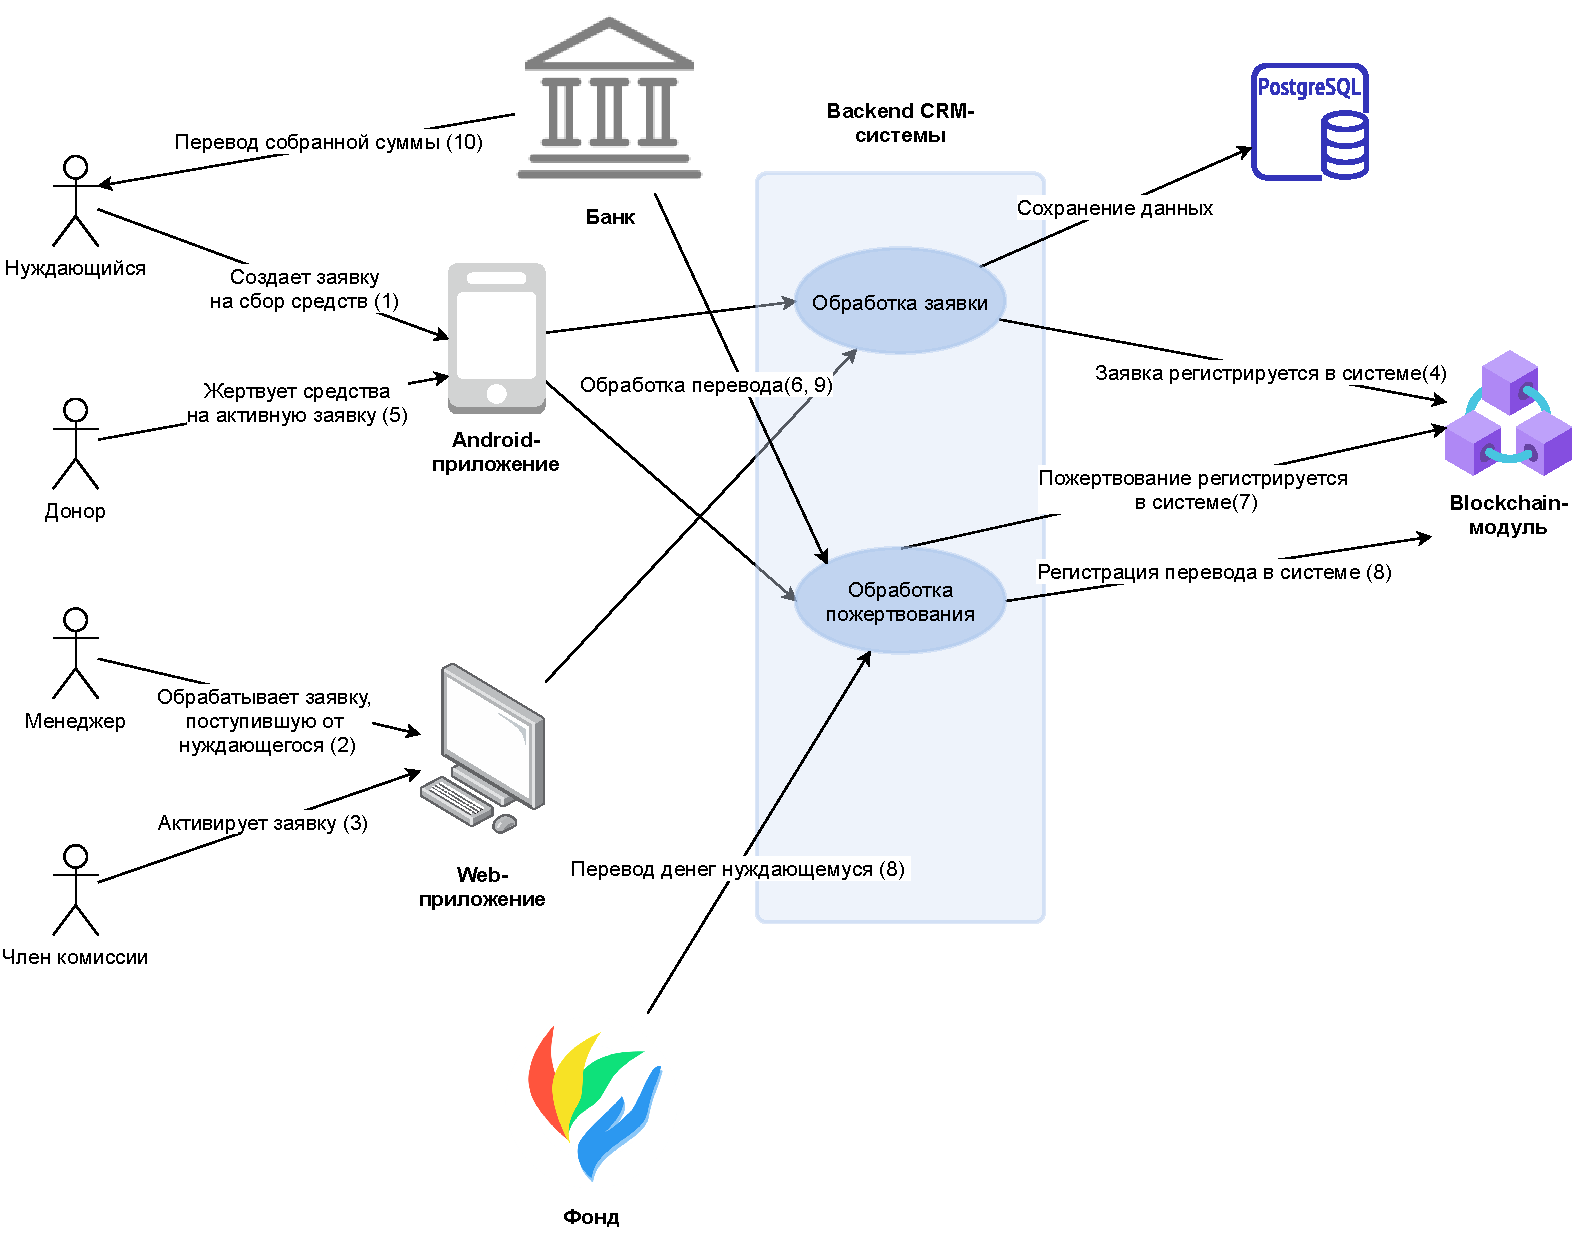
\includegraphics[width = \linewidth]{img/flow.pdf}
		\caption{Взаимодействие частей CRM-системы}
		\label{pic:flow}
\end{figure}


\subsection{Потенциальные пользователи и заинтересованные лица}

\subsubsection{Устройство рынка}

В работе благотворительного фонда задействовано много людей - различные сотрудники фонда, которые обрабатывают поступающие средства и заявки, руководство фонда, бухгалтерия и многие другие. Так как сейчас популярность благотворительных организаций растет с каждым годом, то работа с массовым жертвователем требует отлаженных бизнес-процессов, утверждают эксперты \cite{runok}. 

Прежде чем открывать сбор средств, фонды проводят экспертизу заявок от потенциальных получателей помощи. Этот процесс трудоемкий и требует большого количества ресурсов, так как заявки приходят ручной отбор.  

Также стоит затронуть бизнес процесс учета пожертвований. Самый важный для потенциального жертвователя вопрос – могут ли фонды гарантировать, что деньги потрачены с пользой? Пока единого решения для мониторинга поступающих средств и входящих заявок не существует - большинство фондов ведут учет данных в электронных таблицах. 

Существуют решения в виде CRM-систем для объединенния учета пожертвтвований и заявок. Данные решения доступны по подписке и обычно предоставляют лишь ограниченный фукнционал, который покрывает все бизнес-процессы, специфичные для фонда <<AIAIN>>. 

Таким образом - главное заинтересованное лицо, благотворительная организация <<AIAIN>> не нашла подходящего решения под свои нужды - администрирование персонала, автоматизированное управление и учет заявок и пожертвований, удобная отчетность и аналитика.

\subsubsection{Пользовательская среда}

Разрабатываемый продукт будет применяться сотрудниками фонда <<AIAIN>> в рабочих целях. Продуктом смогут пользоваться как администраторы, менеджеры фонда, так и комиссия по принятию решений. 

Задачи, которые решают пользователи данной системой давольно обширные. Это может быть как обработка заявки и сбор необходимых данных от пользователя, так и более крупные задачи:

\begin{itemize}
    \item Администрирование пользователей системы;
    \item Поддержка пользователей в чате;
    \item Мониторинг и анализ статистики фонда;
    \item Размещение контента о фонде;
    \item Сбор информации о совершенных пожертвованиях, активных донорах фонда; 
\end{itemize}

Перечисленные задачи являются специфичными для предметной области благотворительности и на данный момент фонд их решает с использованием различных систем. Это очень неудобно, так как системы не агрегированы между собой и нет удобного интерфейса для сотрудников фонда.

\subsubsection{Список пользователей} \label{sec: listusers}

В нижеприведенной таблице \ref{table: userlist} можно увидеть описание будущих пользователей системы. Всего сотрудников фонда <<AIAIN>> в штате 12 человек.

\label{subsub: userlist}

\begin{center}
\begin{longtable}{|p{0.2\linewidth}|p{0.35\linewidth}|p{0.4\linewidth}|}
\caption{Список пользователей} 
\label{table: userlist} \\

\hline
\multicolumn{1}{|c|}{\textbf{Роль}} & \multicolumn{1}{c|}{\textbf{Описание}} & \multicolumn{1}{c|}{\textbf{Способ работы}} \\ \hline
\endfirsthead

\multicolumn{3}{r}%
{{ \tablename\ \thetable{} -- продолжение}} \\ 
\hline 
\multicolumn{1}{|c|}{\textbf{Роль}} & \multicolumn{1}{c|}{\textbf{Описание}} & \multicolumn{1}{c|}{\textbf{Способ работы}} \\
\hline
\endhead

\multicolumn{3}{r}{{Продолжение на следующей странице}} \\ 
\endfoot

\hline 
\endlastfoot

Администратор & Сотрудник фонда, задача которого упарвлять пользователями системы, а также мониторить логи. Возраст 20-70 лет. Работает на 1/2 ставку.  & Управляет всеми учетными записями в системе. У него есть доступ к логам системы, а также возможность просматривать пользователей системы и регистрировать их. \\ \hline
Оператор &  Является сотрудником службы поддержки доноров и нуждающихся. Возраст 20-70 лет. Работает на 1/2 ставку. & Отвечает на сообщения пользователей, отправленные через чат. \\ \hline
Контент-менеджер & Отвечает за контент, размещаемый на основной странице фонда. Возраст 20-70 лет. Работает на 1/2 ставку. &  Имеет возможность редактировать описание фонда, а также раздел часто задаваемых вопросов и новости фонда. \\ \hline
Менеджер & Обрабатывает заявки, поступающие в фонд. Возраст 20-70 лет. Полная занятость.  & Имеет доступ к заявкам фонда, а также может обрабатывать данные заявки: менять статусы, редактировать и общаться с пользователем в рамках одной заявки. Также менеджер может просматривать транзакции фонда. \\ \hline
Член комиссии & Члены комиссии фонда принимают решение об опубликовании заявок. Возраст 20-70 лет. Полная занятость. & Имеет доступ к расширенному функционалу управления заявками, а именно к активации заявки (активная заявка становится видимой для всех пользователей системы, на нее можно жертвовать деньги).\\ \hline
\end{longtable}
\end{center}

\subsection{Анализ существующих аналогов}

На этапе анализа необходимо сделать обзор существующих решений, а именно - выделить прямых конкурентов, выявить их сильные стороны и сравнить с разрабатываемым Web-приложением. 

\subsubsection{Краткое описание существующих решений}

При поиске существующих решений была составлена таблица \ref{table: competitors0} с кратким описанием назначения решения и определением типа конкурента \cite{competitors}. При детальном рассмотрении и дальнейшем подробном анализе были выбраны только прямые конкуренты. Жирным шрифтом в таблице \ref{table: competitors0} выделены конкуренты, функциональность которых наиболее пересекается с требованиями, предоставленными заказчиком. Они будут рассмотрены дательно далее.

\begin{longtable}{|p{0.3\linewidth}|p{0.3\linewidth}|p{0.3\linewidth}|} 
\caption{Виды конкурентов} \label{table: competitors0} \\

\hline
\textbf{Название} & \textbf{Описание} & \textbf{Вид} \\ \hline
\endfirsthead

\multicolumn{3}{r}%
{{ \tablename\ \thetable{} -- продолжение}} \\ 
\hline 
\textbf{Название} & \textbf{Описание} & \textbf{Вид} \\
\hline
\endhead

\multicolumn{3}{r}{{Продолжение на следующей странице}} \\ 
\endfoot

\hline 
\endlastfoot

\textbf{Donorfy} &CRM для сбора средств& Прямой \\ \hline
\textbf{DonorPerfect} &Программное обеспечение для сбора средств онлайн& Прямой \\ \hline
\textbf{Beacon} &CRM для благотворительных организаций& Прямой \\ \hline
\textbf{Access thankq} &CRM для благотворительных организаций& Прямой \\ \hline
\textbf{Harlequin charity CRM} &CRM для благотворительных организаций& Прямой \\ \hline
Copper &CRM-система общего назначения& Косвенный \\ \hline
Virtuous &CRM-система, ориентированная на пожертвования и маркетинг& Прямой \\ \hline
Salesforce.com &CRM-система с настраеваемым функционалом& Косвенный \\ \hline
eTapestry &CRM-система для НКО& Прямой \\ \hline
Raiser's edge &CRM-система для НКО& Прямой \\ \hline
CiviCRM &CRM-система для НКО& Прямой \\ \hline
monday.com &CRM платформа общего назначения& Косвенный \\ \hline
Google Sheets &Электронные таблицы& Косвенный \\ \hline
1С &CRM-система& Косвенный \\ \hline
Microsoft Dynamics 365 & CRM-система & Косвенный \\ \hline
Instagram & Социальная сеть&Косвенный \\ \hline
Facebook Fundraisers&Социальная сеть& Косвенный \\ \hline

\end{longtable}


\paragraph*{Donorfy\footnote{\url{https://donorfy.com/features}}\\}

CRM-система для благотоврительный организаций. Используется более чем в 15 фондах, большинство из которых находятся в Дании. Возможна кастомизация функционала, ориентированная на специфику бизнес процессов. Есть интеграция с популярными mailing-сервисами, сервисами по бронированию билетов, PayPal и т.д. Предоставляют функциональные аналитические панели. Поддерживают только три типа пользователя: Administrator, Standard, Viewer. Есть возможность подключить примем пожертвований в виде виджета на веб-сайте. Есть возможность просмотреть поступающие пожертвования от доноров.

\paragraph*{Beacon\footnote{\url{https://www.beaconcrm.org}}\\}


CRM-система для НКО, в рейтинге систем для благотворительных организаций заняла 1 место в 2020 году~\cite{researchcrm}. Предоставляет организациям 14 дней пробного периода, после - оплата каждый месяц. Есть дашборды для сотрудников с задачами. Поддерживает добавление организаций в справочник. Сервис берет комисиию при совершении оплаты через форму на их сайте. Нет поддержки таких ролей как администратор, контент менеджер и оператор.

\paragraph*{Access thankq\footnote{\url{https://www.theaccessgroup.com/charity-crm/}}\\}

CRM-система для НКО из Великобритании, более 10000+ клиентов по всему миру. Функциональность направлена на управление встречами, событиями, а также на мониторинг доноров и волонтеров фонда. Как и предыдущие конкуренты, есть возможность интеграции с популярными платежными сервисами. Предоставляет аналитические панели для мониторинга системы.

\paragraph*{Harlequin charity CRM\footnote{\url{https://www.harlequinsoftware.co.uk/software-services/charity-crm/}}\\}

CRM-система, разработанная в Великобритании. Функциональность ориентирована на небольшие НКО для работы с финансами, а также мониторинг доноров и волонтеров. Только платный функционал. Предлагает настраеваемый интерфейс и функционал.

\paragraph*{DonorPerfect\footnote{\url{https://www.donorperfect.com/fundraising-software/features/}}\\}

CRM система специально для НКО. Имеется мобильное приложение и поддержка пожертвований. Поддерживает ролевую модель сотрудников фонда. Предоставляет только платный функционал, есть аналитические панели.


\subsubsection{Анализ конкурентов}

Взяв за основу критерии (см. изображение \ref{table:research}) из проведенного исследования~\cite{researchcrm} популярных CRM-систем была составлена аналогичная таблица с критериями и метриками, важными в предметной области благотворительности и пожертвований.

\begin{figure}[H]
		\centering
		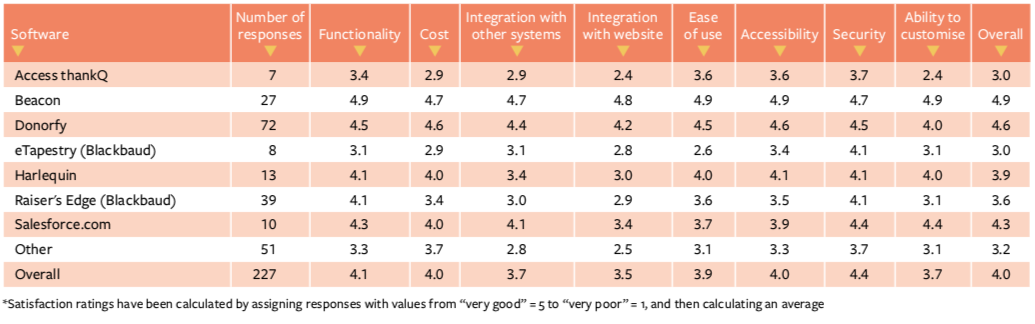
\includegraphics[width = \linewidth]{img/1221.png}
		\caption{Анализ CRM-систем, проведенный в 2020 году}
		\label{table:research}
\end{figure}

При составлении критериев для сравнения были использованы собранные требования от заказчика. Целью данного анализа является выявление сильных сторон конкурентов и внедрение новых требований в разарабатываемый проект. Жирным шрифтом в таблице \ref{table: competitors} выделены ключевые критерии для сравнения.

{

\footnotesize

\begin{longtable}{| >{\raggedright\arraybackslash}p{2.7cm}| >{\centering\arraybackslash}p{2cm}| p{2cm}| p{2cm}| p{2cm}| p{2cm}|}
	\caption{Детальный анализ конкурентов} \label{table: competitors} \\
\hline
& \rotatebox{-90}{\textbf{Donorfy}} & \rotatebox{-90}{\textbf{Beacon}} & \rotatebox{-90}{\textbf{Thankq}} & \rotatebox{-90}{\textbf{Harlequin}} & \rotatebox{-90}
{\textbf{DonorPerfect}} \\ \hline


 \endfirsthead

 \multicolumn{6}{r}%
{{ \tablename\ \thetable{} -- продолжение}} \\ 
\hline 
\endhead

\multicolumn{6}{r}{{Продолжение на следующей странице}} \\ 
\endfoot

\hline 
\endlastfoot

\textbf{Обработка заявок} & 7 & 8 & 8 & 8 & 8  \\ \hline 
\textbf{Ролевая модель} & 6 & 10 & 5 & 5 & 6  \\ \hline 
\textbf{Аналитические панели} & 9 & 9 & 10 & 8 & 8  \\ \hline 
\textbf{Интеграция с мобильным приложением} & 0 & 5 & 0 & 0 & 10  \\ \hline 
\textbf{Администри- рование} & 10 & 10 & 7 & 8 & 8  \\ \hline 
\textbf{Интеграция с блокчейн} & 0 & 0 & 0 & 0 & 0  \\ \hline 
\textbf{Категоризация заявок} & 5 & 7 & 10 & 8 & 10  \\ \hline 
\textbf{Мониторинг пожертвований} & 10 & 10 & 10 & 8 & 8  \\ \hline 
\textbf{Чат поддержки} & 0 & 0 & 0 & 8 & 8  \\ \hline 
\textbf{Управление контентом фонда} & 0 & 0 & 0 & 8 & 8  \\ \hline 
\textbf{Настраеваемые бизнес процессы} & 7 & 6 & 7 & 8 & 8  \\ \hline 
\textbf{Просмотр логов системы} & 10 & 8 & 10 & 8 & 8  \\ \hline 
\textbf{Надежность} & 10 & 10 & 10 & 8 & 8  \\ \hline
\textbf{Пуш уведомления} & 5 & 5 & 10 & 8 & 8  \\ \hline
\textbf{Поддержка нескольких языков} & 0 & 0 & 5 & 5 & 5  \\ \hline
\textbf{Финальная оценка} & \textbf{\scriptsize \kern-0.3em 5,26} & \textbf{\scriptsize \kern-0.3em 7.1} & \textbf{\scriptsize \kern-0.3em 5.9} & \textbf{\scriptsize \kern-0.3em 4.7} & \textbf{\scriptsize \kern-0.3em 6.9} \\ \hline
\end{longtable}
}

Одни из главных требований заказчика было создание заявки от имени фонда на сбор средств для Закята (см. раздел определений). Для этого необходим следующий функционал: создание заявок от имени фонда, а также категоризация заявок (и управление категориями).

Так как при анализе конкурентов упор делался на следующий функционал: обработка заявок, категоризация заявок, администрирование, пуш уведомление, мультиязычность и ролевая модель, то при подсчете финальной оценки был применен следующий алгоритм: 

Критерии оценки были разбиты на следующие группы, так как для каждой категории был задан вес (от 0 до 10, где 10 -- самое важное) по важности: 
\begin{enumerate}
	
	\item Функционал по обработке заявок -- 10
	\item Наличие функционала по администрированию пользователями платформы -- 10
	\item Наличие функционала по обработке заявок -- 9
	\item Категоризация заявок -- 9
	\item Ролевая модель -- 9
	\item Наличие пуш уведомлений -- 8
	\item Мониторинг пожертвований -- 8
	\item Аналитические панели -- 8
	\item Интеграция с системой блокчейн -- 8
	\item Интеграция с мобильным приложением -- 8
	\item Чат поддержки -- 7
	\item Настраеваемые бизнес-процессы -- 9
	\item Просмотр логов системы -- 6
	\item Надежность -- 9
	\item Поддержка нескольких языков -- 10
\end{enumerate}

Далее при подсчете финальной оценки применялся метод подсчета взвешенного среднего арифметического\footnote{\url{https://en.wikipedia.org/wiki/Weighted_arithmetic_mean}}. 

\subsection{Преимущества ПО по сравнению с аналогами}

Таким образом, можно сделать следующие выводы:
\begin{itemize}
    \item Функциональсть администратора должна предполагать управление пользователями системы, а также должна быть возможность заблокировать пользователей системы и тем самым ограничить их доступ в систему;
    \item Необходима функциональность по управлению информацией о фонде (описание, документы, часто задаваемые вопросы) - такого не представленно ни в одной из перечисленных CRM систем, так как только одна из них  интегрирована с мобильным приложением для пользователей;
    \item Уведомления сотрудников фонда о действиях в системе - очень важная часть, в большинстве существующих CRM-систем реализована через email-рассылки или интеграции со сторонними сервисами (настраеваемый функционал);
    \item Очень важны аналитические панели - корректная и правильная аналитика должна дать сотрудникам фонда представление о статистике собранных средств; В некоторых существующих решениях есть возможность настроить аналитические панели и демонстрировать только релевантную информацию;
\end{itemize}

\anonsubsection{Выводы по главе}

В рамках аналитической стадии разработки был проведен анализ устройства рынка, будущих пользователей. Также были выявлены существующие аналоги: они были разделены на косвенных и прямых конкурентов разрабатываемого Web-приложения. Глубокий анализ основных конкурентов позволил выявить слабые стороны Web-приложений в сфере программного обеспечения для управления деятельностью благотворительных фондов. Это позволило скоректировать требования, описанные в техническом задании (см. Приложение~\ref{additiontz}).

\clearpage
\newpage


\setcounter{section}{2}
\setcounter{subsection}{0}

\sectionVKR{Описание разработанных моделей и алгоритмов}

\subsection{Сценарии использования} \label{usecase}

На этапе проектирования была смоделирована диаграмма прецедентов по стандартам UML\cite{uml}. Перед составлением диаграммы были перечислены основные разделы приложения со следующим функционалом:
\begin{itemize}
    \item Личный профиль -- раздел по управлению личным профилем и настройками приложения (выбор языка, разрешение пуш-уведомлений);
    \item Заявки -- полная обработка поступающих заявок на пожертвования (бизнес процесс описан в разделе \ref{sec: application}), а также голосование членов комиссии по заявка (этот бизнес процесс подробно описан в пункте \ref{sec: vote});
    \item Уведомления -- раздел пуш-уведомлений, а также получения информации о смене статусов обрабатываемых заявок в системе блокчейн;
    \item Пожертвования -- раздел с мониторингом пожертвований, поступающих от пользователя;
    \item Управление пользователями -- мониторинг и управление пользователями системы, редактирование и регистрация в системе;
    \item Управление контентом фонда -- управление информацией о фонде, разделом <<Часто задаваемые вопросы>> и <<Новости>>;
    \item Чат поддержки с пользователями -- раздел диалогов с пользователями;
\end{itemize}

На диаграмме \ref{pic: usecase} отражены основные юзкейсы работы системы, а также приведены акторы, которые взаимодействуют с системой. В нижеприведенной таблице \ref{table:actors} представлены подробные описания каждого актора.

\begin{center}
\begin{longtable}{|p{0.15\linewidth}|p{0.75\linewidth}|}
\caption{Акторы диаграммы прецедентов} \label{table:actors} \\

\hline \multicolumn{1}{|c|}{\textbf{Актор}} & \multicolumn{1}{c|}{\textbf{Описание}} \\ \hline
\endfirsthead

\multicolumn{2}{r}%
{{\bfseries \tablename\ \thetable{} -- продолжение таблицы}} \\
\hline \multicolumn{1}{|c|}{\textbf{Актор}} & \multicolumn{1}{c|}{\textbf{Описание}} \\ \hline 
\endhead

\hline \multicolumn{2}{r}{{Продолжение на следующей странице}} \\ 
\endfoot

\hline \hline
\endlastfoot

General user & Обобщение для всех пользователей CRM. \\ \hline
Admin & \textbf{Администратор} управляет всеми учетными записями в системе. У него есть доступ к логам системы, а также возможность просматривать пользователей системы и регистрировать их. \\ \hline
Operator & \textbf{Оператор} отвечает на сообщения пользователей, отправленные через чат. \\ \hline
Content Manager & 
\textbf{Менеджер контента} системы имеет возможность редактировать описание фонда, а также раздел часто задаваемых вопросов. \\ \hline
Manager & \textbf{Менеджер фонда} имеет доступ к заявкам фонда, а также может обрабатывать данные заявки: менять статусы, редактировать и общаться с пользователем в рамках одной заявки. Также менеджер может просматривать транзакции фонда. \\ \hline
SuperManager & \textbf{Комиссия фонда} имеет доступ к расширенному функционалу управления заявками, а именно к активации заявки (активная заявка становится видимой для всех пользователей системы, на нее можно жертвовать деньги). \\ \hline
Firebase & Система рассылки уведомлений. \\ \hline





\end{longtable}
\end{center}

\begin{figure}[H]
		\centering
		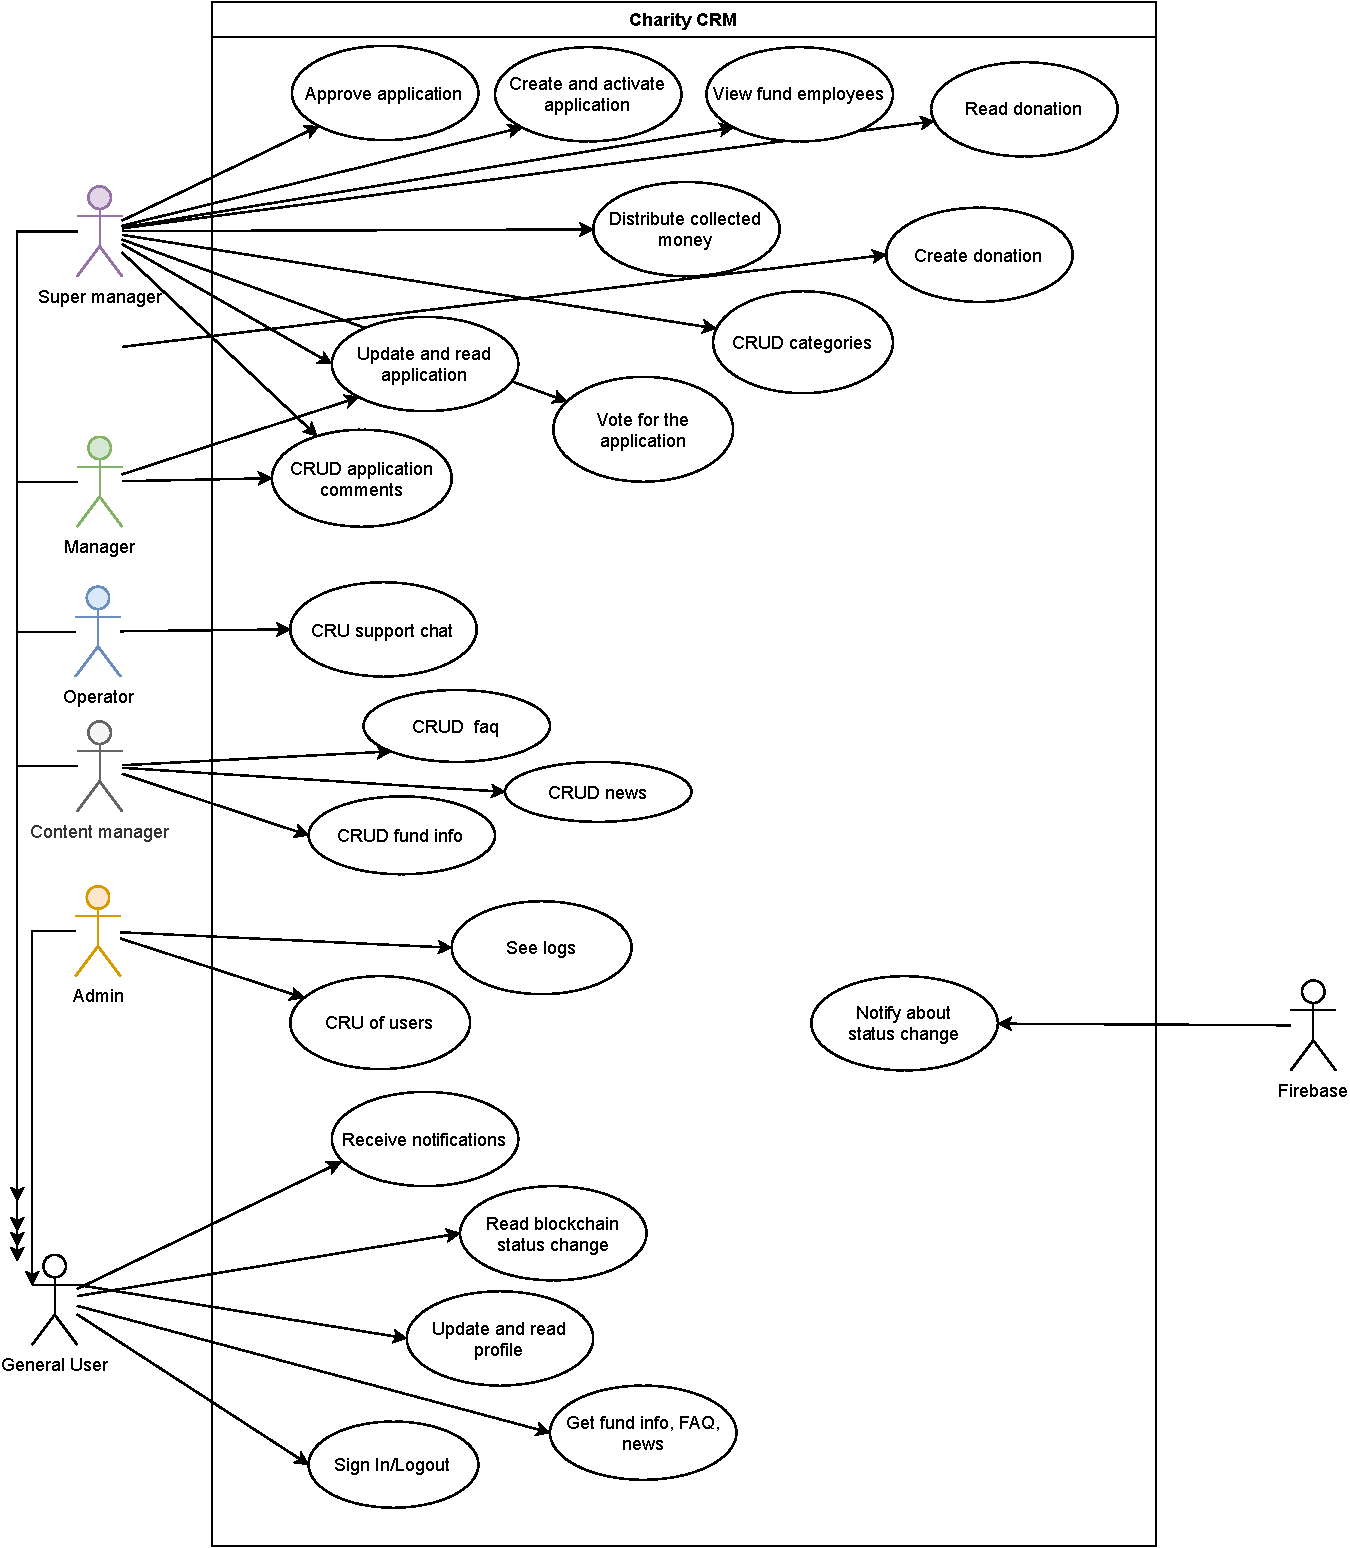
\includegraphics[width = 0.9\linewidth]{img/usecase.pdf}
		\caption{Диаграмма прецедентов}
		\label{pic: usecase}
\end{figure}




Также было составлено краткое описание каждого юзкейса в таблице \ref{table:usecase}.

\begin{center}
\begin{longtable}{|p{0.1\linewidth}|p{0.15\linewidth}|p{0.15\linewidth}|p{0.45\linewidth}|}
\caption{Акторы диаграммы прецедентов} \label{table:usecase} \\

\hline
\multicolumn{1}{|c|}{\textbf{№}} & \multicolumn{1}{c|}{\textbf{Название}} & \multicolumn{1}{c|}{\textbf{Актор(ы)}} & \multicolumn{1}{c|}{\textbf{Описание}} \\ \hline
\endfirsthead

\multicolumn{4}{r}%
{{ \tablename\ \thetable{} -- продолжение}} \\
\hline 
\multicolumn{1}{|c|}{\textbf{№}} & \multicolumn{1}{c|}{\textbf{Название}} & \multicolumn{1}{c|}{\textbf{Актор(ы)}} & \multicolumn{1}{c|}{\textbf{Описание}} \\ 
\hline
\endhead

\hline \multicolumn{4}{r}{{Продолжение на следующей странице}} \\
\endfoot

\hline \hline
\endlastfoot

\multicolumn{4}{|c|}{\textbf{Аутентификация}} \\ \hline

1 & Sign In & General User & 
Авторизация всех пользователей в приложении происходит с помощью ввода почты и пароля, указанных при регистрации в системе \\ \hline


\multicolumn{4}{|c|}{\textbf{Управление пользователями}} \\ \hline

2 & CRU of users & Admin & 
Создание, редактирование, просмотр пользователей системы. Администратор имеет возможность: зарегистрировать пользователя в системе, просмотреть список пользователей и информацию о каждом, изменить информацию: заблокировать или разблокировать пользователя;  \\ \hline

3 & See logs & Admin & Просмотр действий пользователей в системе: авторизация, действия по заявкам, совершенные пожертвования и т.д;
 \\ \hline
 
4 & View fund employees & Supermanager & Член комиссии имеет возможность просматривать информацию о сотрудниках фонда, а также их заявки \\ \hline
 
\multicolumn{4}{|c|}{\textbf{Заявки}} \\ \hline

5 & CRUD application comments & Manager, Supermanager & Менеджер, комиссия и пользователь могут оставлять комментарии под заявками. Менеджер и комиссия могут это делать для всех заявок. \\ \hline

6 & Approve application & Supermanager & Комиссия может одобрять заявки, таким образом они становятся активны и на них пользователи могут жертвовать деньги, после одобрения заявка передается в блокчейн. \\ \hline

7 & Update and read application & Manager & Менеджер может просматривать заявки, а также переводить заявки в разные статусы, редактировать ее. \\ \hline

8 & Create and activate application & Supermanager & Член комиссии имеет возможность создать заявку за другого человека, при создании заявки она автоматически появляется в реестре как активная \\ \hline

9 & Vote fot the application & Supermanager & Член комиссии, назначенные категории которого совпадают с категорией заявки, имеет возможность проголосовать за или против активации заявки \\ \hline

\multicolumn{4}{|c|}{\textbf{Пожертвования}} \\ \hline

10 & Read donation & Supermanager & Комиссия фонда может просматривать все совершенные транзакции в рамках системы.
 \\ \hline
 
11 & Distribute collected money & Supermanager & Комиссия фонда может направить собранные средства со счета фонда на одну из заявок.
 \\ \hline
 
12 & Create donation & Supermanager & Комиссия фонда может создать запись о пожертвовании, совершенном вне системы. \\ \hline

\multicolumn{4}{|c|}{\textbf{Личный профиль}} \\ \hline

13 & Update and read profile & General User & Все пользователи системы могут просматривать информацию о себе, а также ее менять. \\ \hline

\multicolumn{4}{|c|}{\textbf{Категории}} \\ \hline

14 & CRUD categories & Supermanager & Суперменеджеры могут изменять категории, которые ассоциируются с заявками. \\ \hline

\multicolumn{4}{|c|}{\textbf{Информация о фонде, чаты}} \\ \hline

15 & CRU support chat & Operator & При возникших вопросах пользователь приложения может обратиться за помощью, написав в чат, где операторы ответят на все его интересующие вопросы. \\ \hline

16 & CRU fund info & Content manager & Контент-менеджер может редактировать информацию о фонде \\ \hline

17 & CRU faq & Content manager & Контент-менеджер может редактировать часто задаваемые вопросы о фонде \\ \hline

18 & CRU news & Content manager & Контент-менеджер может редактировать новостную ленту \\ \hline

19 & Get fund info, FAQ, news & General User & Пользователи системы могут получить информацию о фонде \\ \hline

\multicolumn{4}{|c|}{\textbf{Нотификации}} \\ \hline

20 & Notify about status change & Firebase & Рассылка уведомлений об изменении статуса заявки пользователю, создавшему заявку. \\ \hline

21 & Receive notifications & General User & Пользователь может получать нотификации от системы. \\ \hline

22 & Read blockchain status change & General User & Пользователь может просматривать информацию о смене статусов операций в системе. \\ 

\end{longtable}
\end{center}

\subsection{Модель предметной области} \label{sec: application}

На этапе анализа была разработана диаграмма предметной  области \ref{pic: domain} разрабатываемого приложения по стандартам UML\cite{uml}. Как упоминалось ранее в Главе 1, разрабатываемое приложение направлено на интересы сотрудников фонда и самого фонда. 

Так как модель предметной области представляет собой совокупность понятий предметной области и отношений между ними (т.е. совокупность поведения и данных), то при ее разработке я в первую очередь руководствовалась use-case диаграммой~ \ref{pic: usecase}, а также бизнес-правилами из документа <<Техническое задание. CRM-система для благотворительного фонда <<AIAIN>>. Web-приложение для сотрудников фонда>> (см. Приложение~\ref{additiontz}). В целом главной чертой, отличающей одну модель предметной области от другой, является именно набор бизнес-правил.

В следующем разделе детально рассмотрен бизнес-процесс обработки заявки (см. диаграмму \ref{pic: status}), но стоит упомянуть, что все нюансы процесса также были отражены на диаграмме предметной области: для каждой роли был введен свой класс (например \texttt{Manager}, \texttt{Operator}) и разграничены возможности пользователей взаимодействия с заявками, чатами, новостным контентов и так далее.

В процессе разработки модель предметной области дополнялась в соответствии с развивающейся системой и изменяющимися требованиями заказчика. 

\begin{figure}[H]
		\centering
		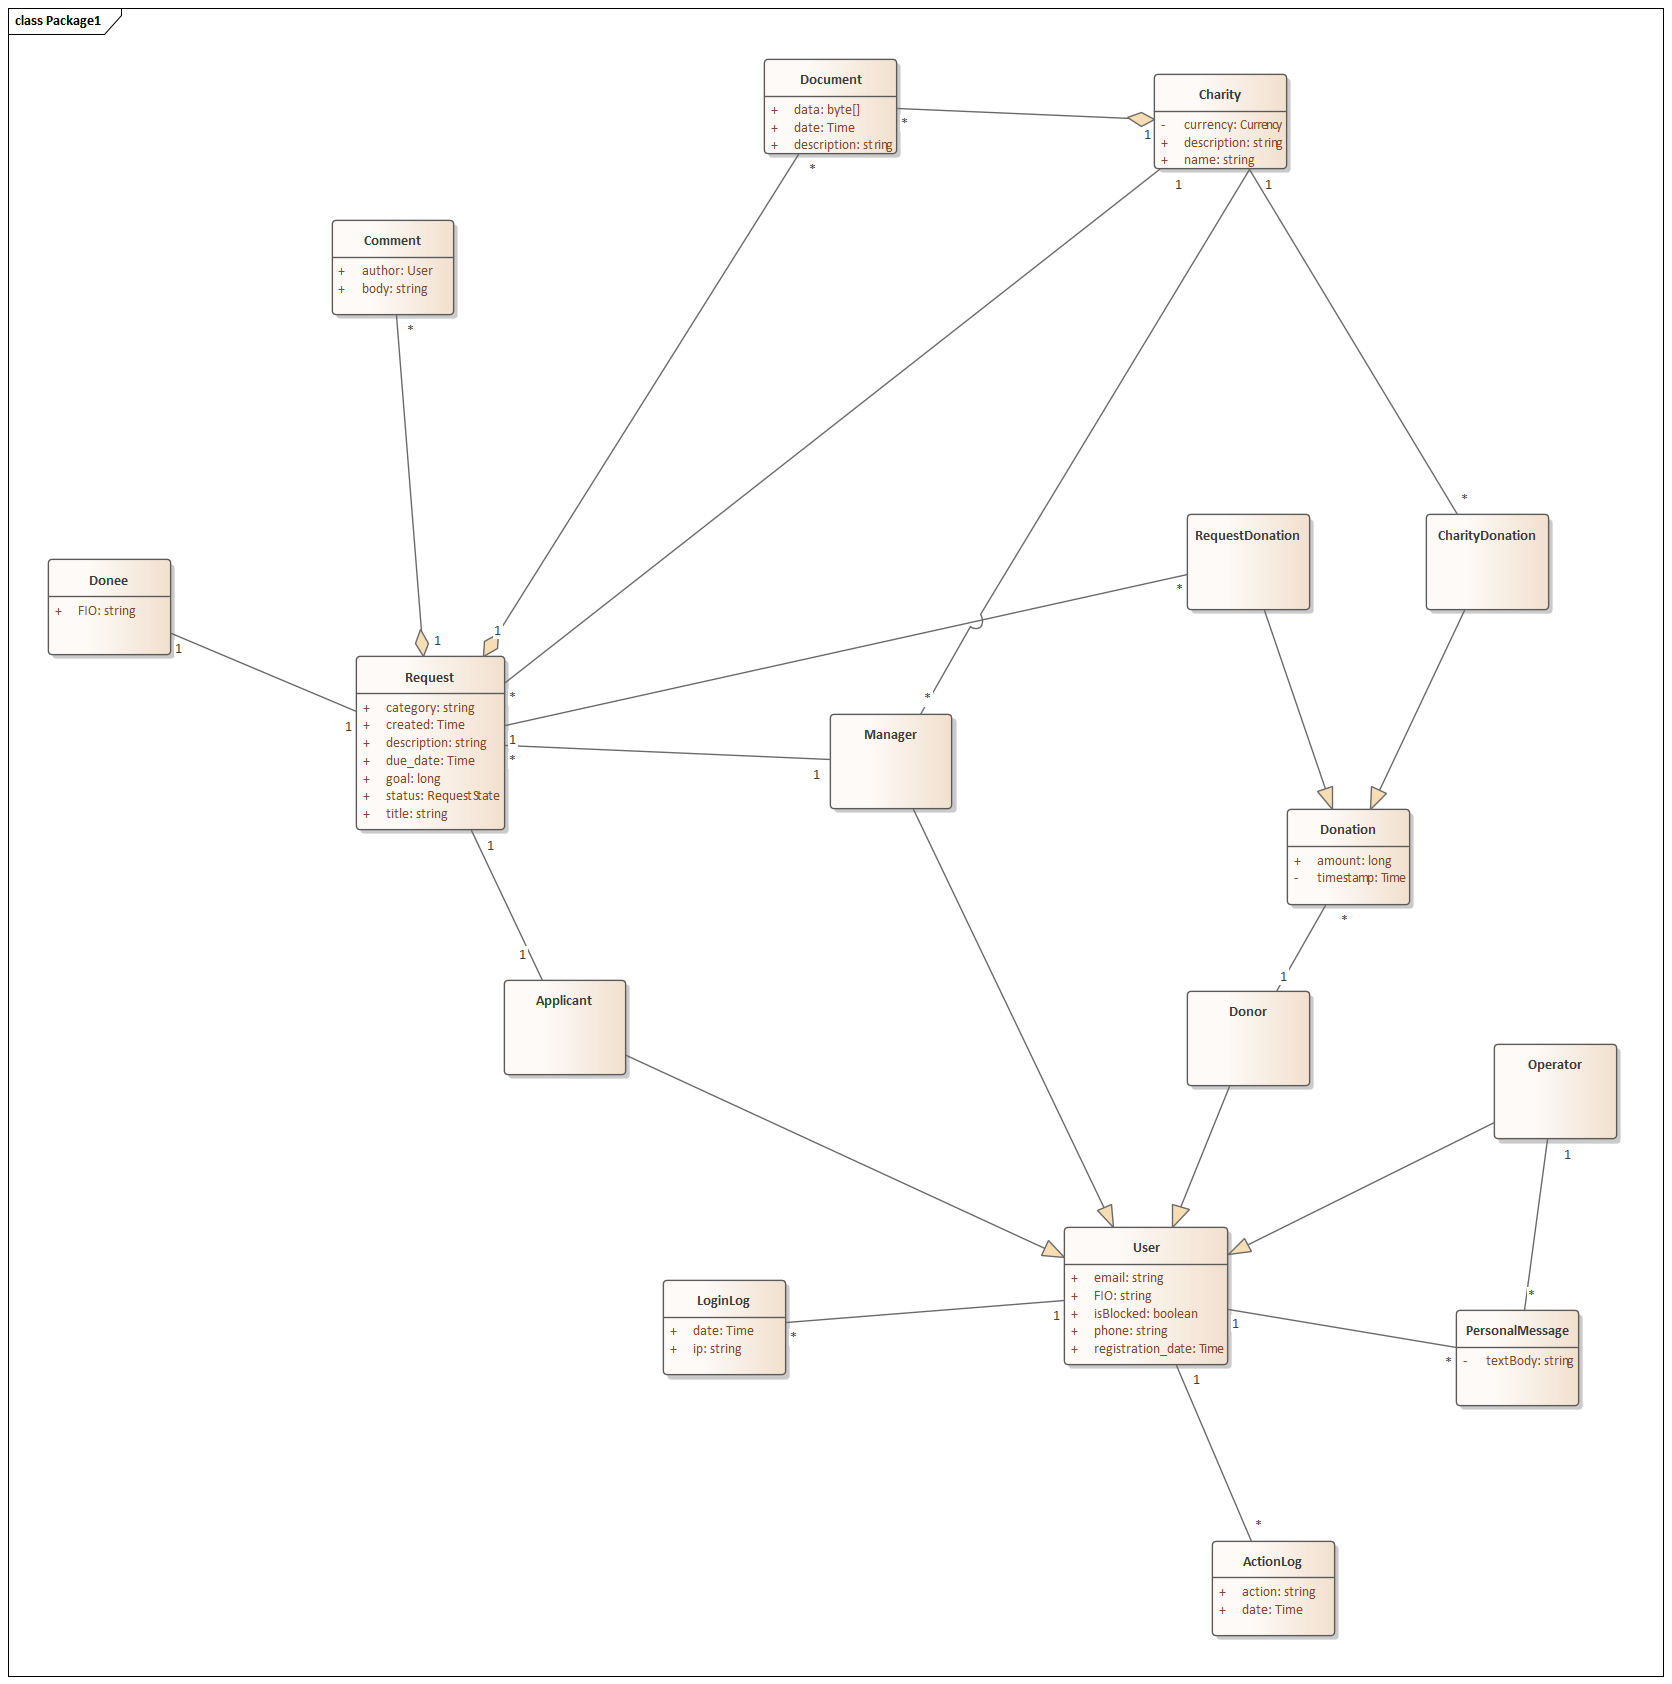
\includegraphics[width = 0.9\linewidth]{img/domain.png}
		\caption{Диаграмма предметной области}
		\label{pic: domain}
\end{figure}

\subsection{Модель обработки заявки} \label{sec: bpmn_status}


При моделировании бизнес процесса обработки заявки от пользователя на сбор средств была составлена диаграмма Business Process Model and Notation (BPMN~\cite{bpmn}), в которой был смоделирован бизнес-процесс и показано, как модули CRM-системы взаимодействуют между собой (см. диаграмму \ref{pic: bpmn_1}).

\begin{figure}[H]
		\centering
		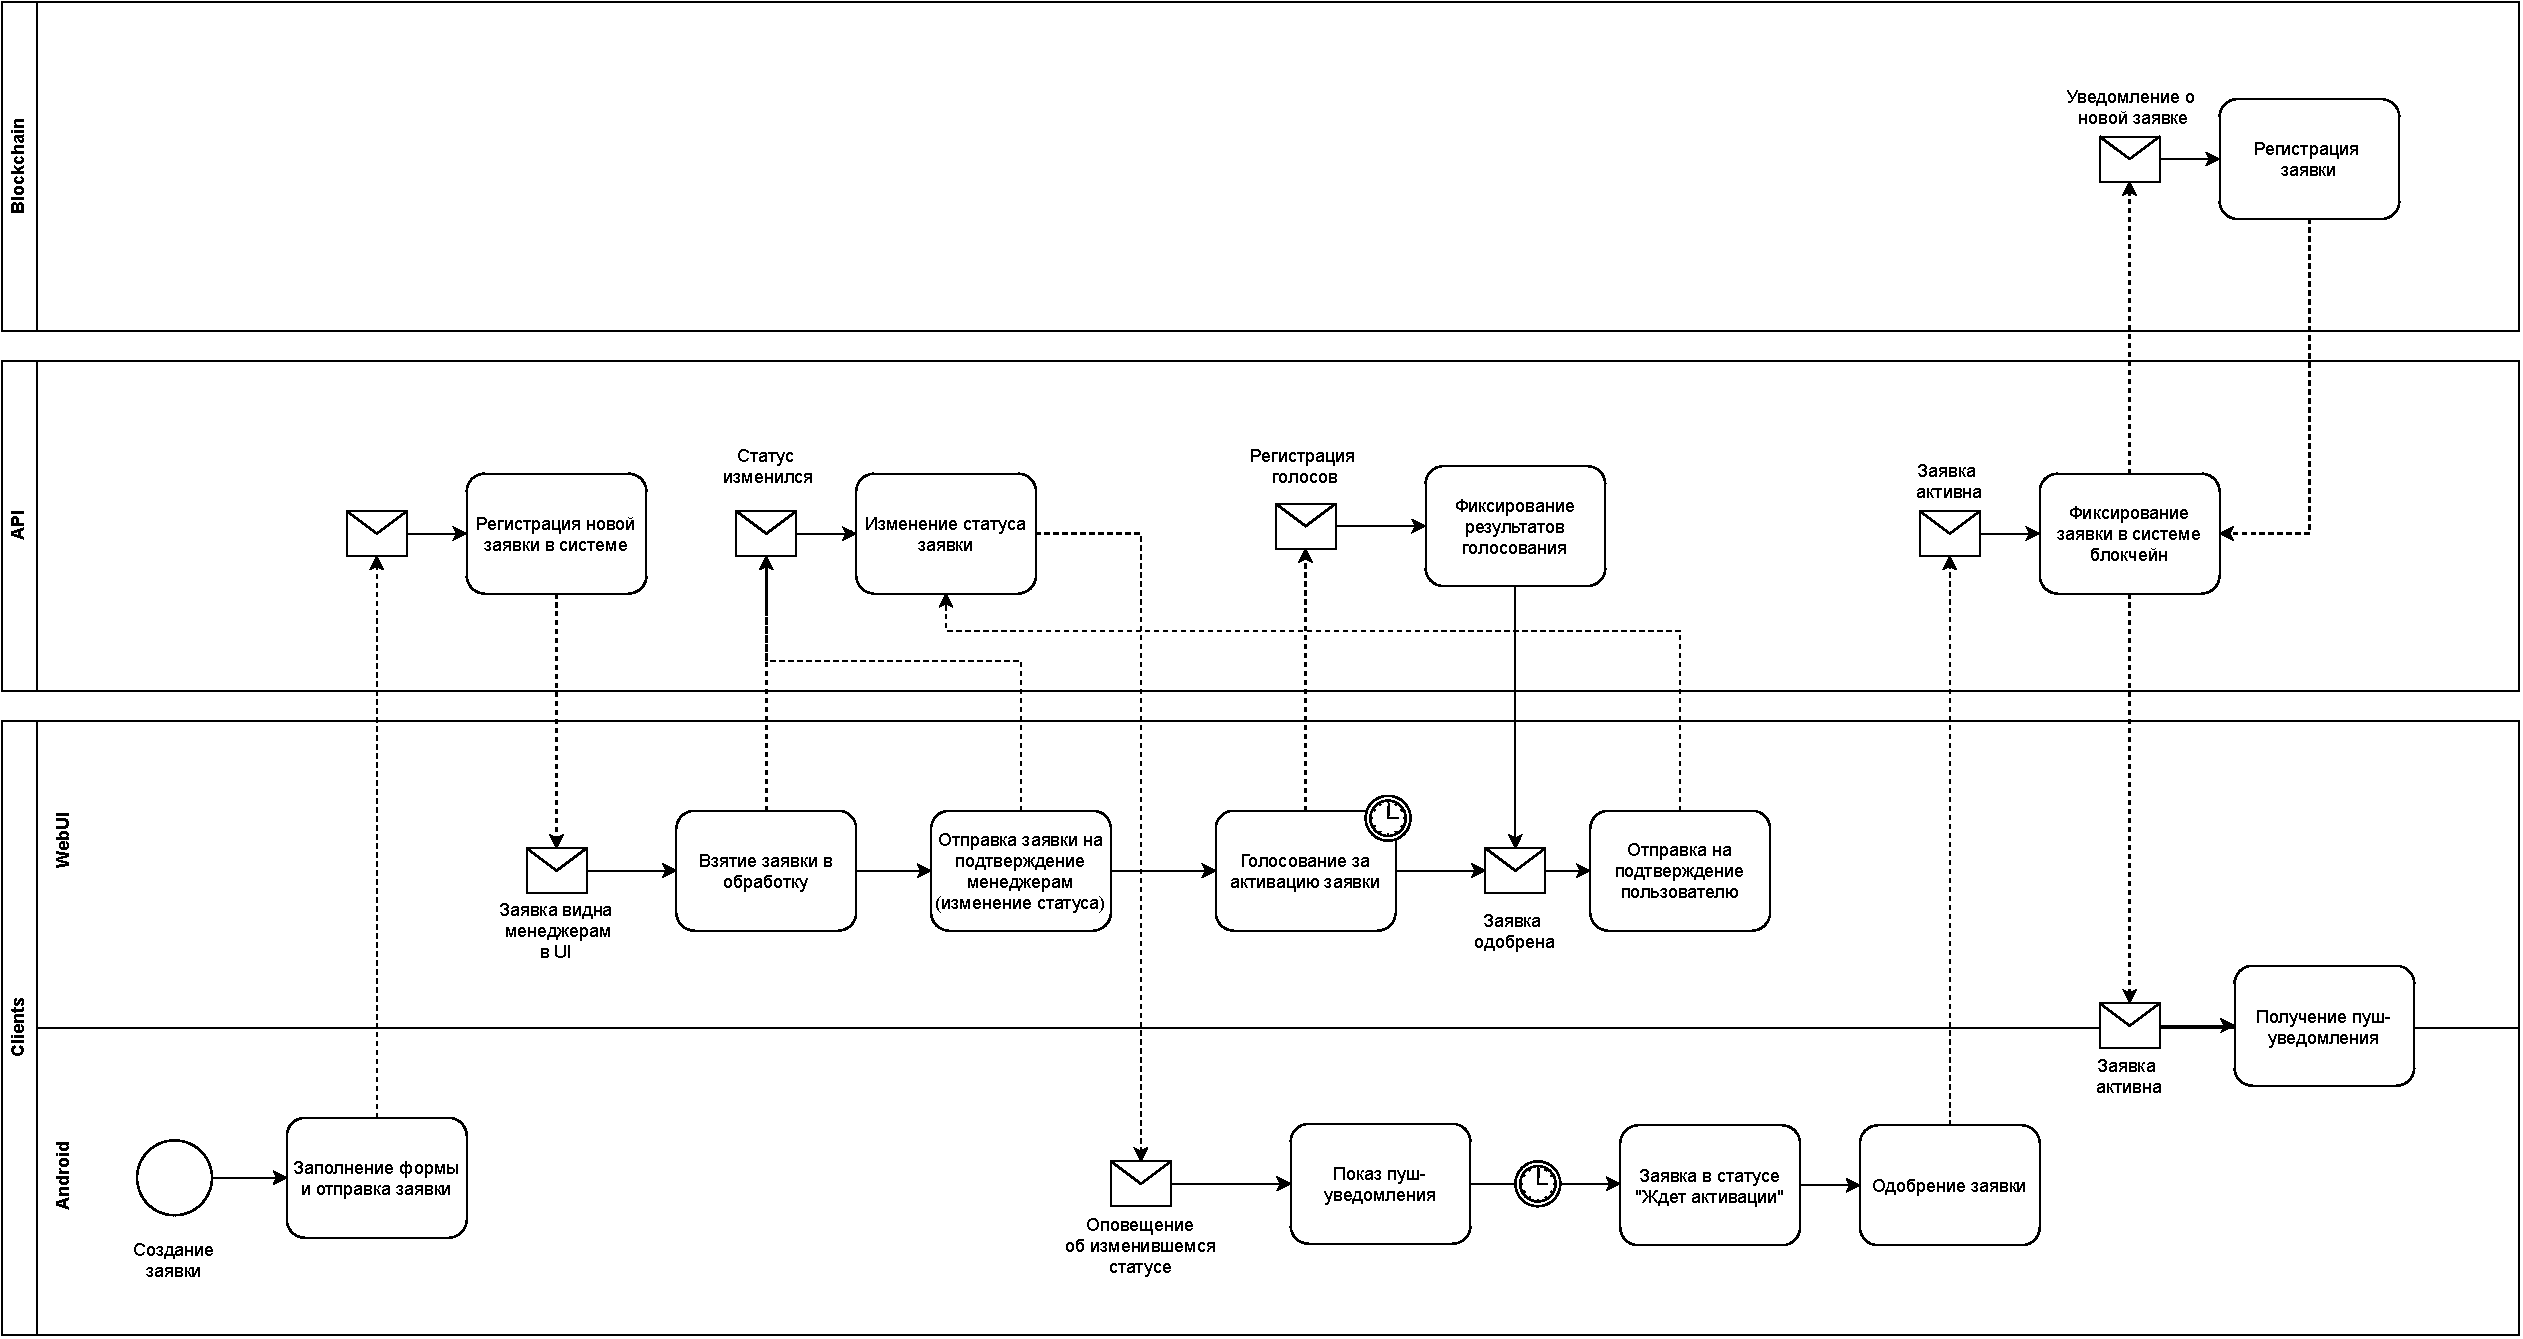
\includegraphics[width = \linewidth]{img/bpmn_status.pdf}
		\caption{BPMN обработки заявки всей системы}
		\label{pic: bpmn_1}
\end{figure}

Подробная диаграмма взаимодейтсвия данного бизнес процесса представлена в разделе \ref{sec: sequence_status} главы 3. Рассмотрим подробнее, что происходит на диаграмме \ref{pic: bpmn_1} бизнес-процесса обработки заявок. Пользователь мобильного приложения (нуждающийся) создает заявку в мобильном приложении, созданная заявка в статусе <<Новая>> (подробнее модель статусов рассмотрена ниже в разделе, в таблице \ref{table: status}) заносится в базу данных через API системы. В Web-интерфейсе сотрудника фонда появляется только что созданная заявка, которую сотрудник с ролью <<Член комиссии>> или <<Менеджер>> (все роли пользователей представлены в разделе \ref{sec: listusers}) берет в обработку. Статус заявки меняется на <<В обработке>> и изменения также заносятся в базу данных через API системы. При каждом изменении статуса заявки мобильный пользователь получает пуш-уведомления. Далее происходит голосование по заявке, бизнес процесс которого описан в разделе \ref{sec: vote}, а полная диаграмма последовательности в разделе \ref{sec: vote_seq}. После принятия положительного решения сотрудник фонда отправляет заявку на финальное подтверждение пользователю, все изменения заносятся в базу данных. Пользователь мобильного приложения одобряет заявку, данные изменения фиксируются в базе данных, заявка заносится в систему блокчейн. Оба пользователя (сотрудник фонда и нуждающийся) получают пуш-уведомления об успешной активации заявки.


Также была проработана более упрощенная модель обработки заявки непосредственно для Web-приложения, чтобы выделить непосредственные шаги, которые должны быть проведены членом комиссии для активации заявки, см. диаграмму \ref{pic: short_bpmn}. 

\begin{figure}[H]
		\centering
		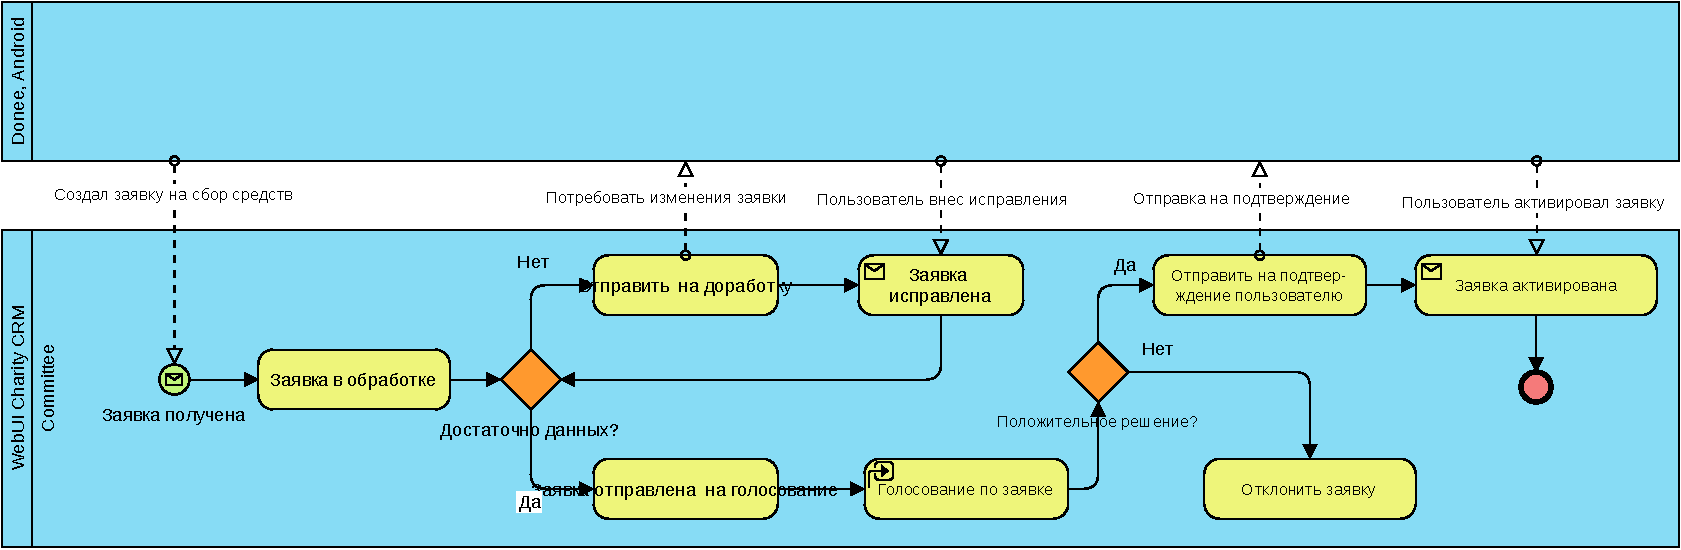
\includegraphics[width = \linewidth]{img/BPMN_web_status.pdf}
		\caption{Диаграмма BPMN, упрощенная версия для Web-приложения}
		\label{pic: short_bpmn}
\end{figure}


На этапе анализа была проработана модель обработки заявки на сбор средств. Так как обработка заявки на сбор средств является главной функциональностью пользователей с ролями <<Менеджер>>, <<Член комиссии>>, то была составлена диаграмма \ref{pic: status} состояний для сущности <<заявка на пожертвование>>. 

\begin{figure}[H]
		\centering
		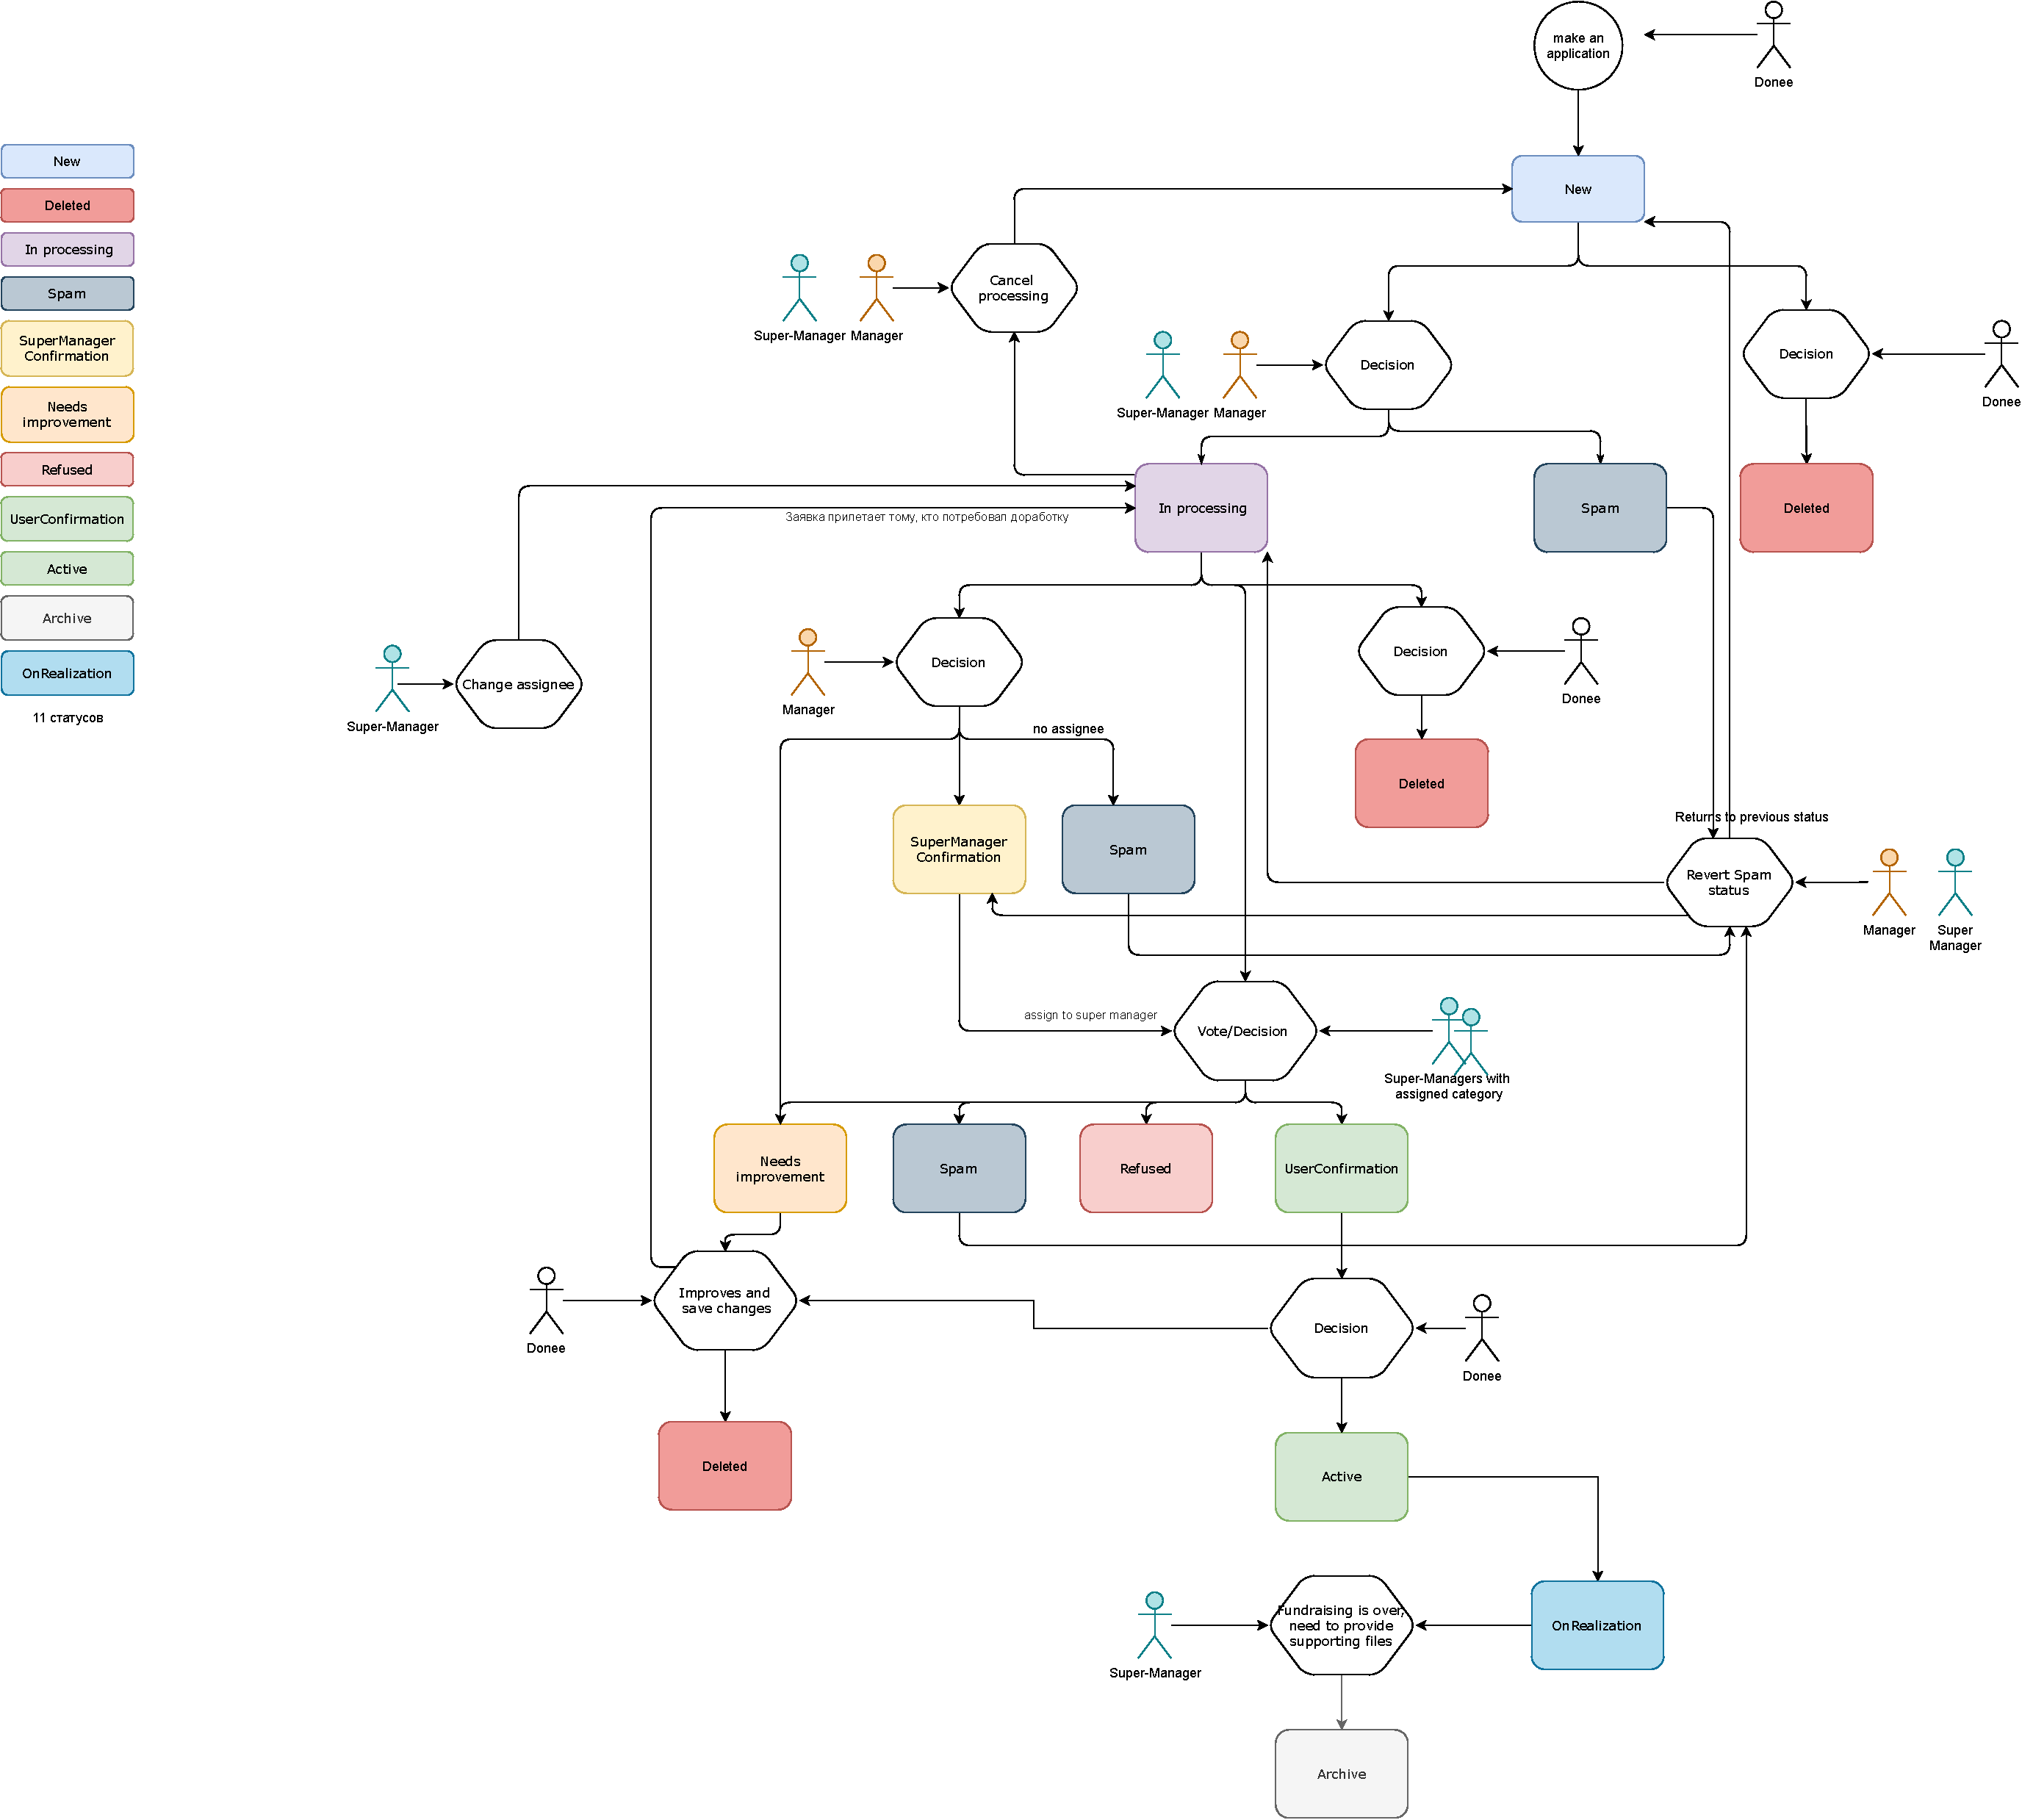
\includegraphics[width = 0.9\linewidth]{img/statusflow.pdf}
		\caption{Диаграмма статусов}
		\label{pic: status}
\end{figure}


При сборе требований заказчик сделал упор на бизнес-процесс обработки заявки, а именно: ограничение прав на совершение определенных переходов заявки (прим. обычный менеджер не может активировать заявку), а также на ограничение доступных статусов для перехода на каждом этапе заявки. Таблица \ref{table: statusflow} отражает разграничение действий по ролям и органичения на переходы статусов. Описание статусов представлено в таблице \ref{table: status}.


\begin{center}
\begin{longtable}{|C{30mm}|C{30mm}|*{2}{C{30mm}|}}  % set suitable column widths

\caption{Переходы заявки в различные статусы}

\hline
& & \multicolumn{2}{c|}{\textbf{Статус}} \\
\cline{3-4}
\textbf{Кто} & \textbf{Действие} & \multicolumn{1}{c|}{\textit{Предыдущий}} & \multicolumn{1}{c|}{\textit{Следующий}} \\ \hline
\endfirsthead

\multicolumn{4}{r}%
{{ \tablename\ \thetable{} -- продолжение}} \\ 
\hline 
& & \multicolumn{2}{c|}{\textbf{Статус}} \\
\cline{3-4}
\textbf{Кто} & \textbf{Действие} & \multicolumn{1}{c|}{\textit{Предыдущий}} & \multicolumn{1}{c|}{\textit{Следующий}} \\ \hline
\endhead

\hline
\multicolumn{4}{r}{{Продолжение на следующей странице}} \\ 
\endfoot

\hline 
\endlastfoot
\label{table: statusflow}

Менеджер & \multirow{2}{30mm}{Взятие заявки в обработку} & \multirow{2}{*}{Новая} & \multirow{2}{*}{В обработке} \\ \cline{1-1}
Член комиссии & & & \\ \hline

\multirow{2}{30mm}{Член комиссии} & \multirow{2}{30mm}{Отклонение заявки} & \multirow{1}{*}{В обработке} & \multirow{2}{*}{Отклонена} \\ \cline{3-3}
& & Ждет активации & \\ \hline


Менеджер & \multirow{2}{30mm}{Отправление заявки на доработку} & В обработке & На доработке \\ \cline{1-1} \cline{3-4}
\multirow{2}{30mm}{Член комиссии} & & Ждет активации & \multirow{2}{*}{На доработке} \\ \cline{3-3}
 & & В обработке & \\ \hline
 
Менеджер & Отправление заявки на активацию / отклонение & В обработке & Ждет активации \\ \hline

\multirow{2}{30mm}{Член комиссии} & \multirow{2}{30mm}{Активация заявки} & Ждет активации & \multirow{2}{30mm}{Ждет подтверждения} \\ \cline{3-3}

 & & В обработке & \\ \hline
 
\multirow{2}{30mm}{Менеджер} & \multirow{3}{30mm}{Пометка заявки как спам} & Новая & \multirow{3}{*}{Спам} \\ \cline{3-3}

& & В обработке & \\ \cline{1-1} \cline{3-3} 
Член комиссии & & Ждет активации & \\ \hline

Член комиссии & Закончился сбор средств (либо автоматически закрывается сбор) & Активная & Архив \\ \hline

Член комиссии & \multirow{3}{30mm}{Вернуть заявку статуса "спам" в предыдущий} & \multirow{3}{30mm}{Спам} & Новая \\ \cline{1-1} \cline{4-4} 

\multirow{2}{30mm}{Менеджер} & & & В обработке \\ \cline{4-4}

& & & Ждет активации \\ \hline


Менеджер & \multirow{2}{30mm}{Отказаться от обработки} & \multirow{2}{*}{В обработке} & \multirow{2}{*}{Новая} \\ \cline{1-1}

Член комиссии & & & \\ \hline


Менеджер & \multirow{2}{30mm}{Отменить доработку} & \multirow{2}{*}{На доработке} & В обработке \\ \cline{1-1} \cline{4-4}

Член комиссии & & & Ждет активации \\ \hline

Член комиссии & Изменение assignee у заявки & В обработке & В обработке \\ \hline

\end{longtable}
\end{center}

\begin{longtable}[]{|@{\textbf}r|p{3.5cm}|p{3.5cm}|p{7cm}|} 
\caption{Статусы заявки}

\hline
\textbf{№} & \textbf{Название статуса на английском} & \textbf{Название статуса на русском} & \textbf{Описание} \\ \hline
\endfirsthead

\multicolumn{4}{r}%
{{ \tablename\ \thetable{} -- продолжение}} \\ 
\hline 
\textbf{№} & \textbf{Название статуса на английском} & \textbf{Название статуса на русском} & \textbf{Описание} \\
\endhead

\multicolumn{4}{r}{{Продолжение на следующей странице}} \\ 
\endfoot

\hline 
\endlastfoot
\label{table: status}
    1 & New & Новая            &  Только что созданная заявка от пользователя \\ \hline
    2 & In progress & В обработке            &  Заявка находится в обработке у одного из менеджеров. Пока заявка в этом статусе, менеджер просматривает документы и удостоверивается в подлинности заявки. \\ \hline
    3 & Spam & Спам            & Заявка помечена как спам. \\ \hline
    4 & Needs Improvement & На доработке & Не указано достаточно данных для подтверждения заявки, менеджеру требуются дополнительные сведения, он может оставить комментарий - причину отказа. Есть возможность отредактировать.  \\ \hline
    5 & Archieved &  Архив & Заявка либо устарела, либо деньги были собраны. \\ \hline
    6 & Rejected &  Отказано & Отказано в рассмотрении заявки; \\ \hline
    7 & Active &  Активная & Заявка прошла все стадии подтверждения и открыта к сбору средств; \\ \hline
    8 & Supermanager Confirmation &  На подтверждении у комиссии & Прежде чем быть опубликованной, заявка должна быть одобрена членом комиссии; \\ \hline
    9 & User Confirmation &  На подтверждении у пользователя & Прежде чем быть опубликованной, финальная версия заявки должна быть одобрена пользователем; \\ \hline
    10 & Deleted & Удалена & Пользоатель имеет право удалить свою заявку, таким образом она больше не будет рассматриваться менеджерами и претендовать на публикацию; \\ \hline
    11 & OnRealization & В реализации & Фонд перечислил средства нуждающемуся, но деньги еще не пошли на благое дело (не были получены документы, подтверждающие реализацию средств); \\ \hline
\end{longtable}


\subsection{Модель голосования по заявке} \label{sec: vote}

При моделировании бизнес процесса голосования по заявке членами комисии, чьи назначенные категории совпадают с категорией заявки, была составлена диаграмма Business Process Model and Notation (BPMN~\cite{bpmn}), в которой был смоделирован бизнес-процесс и показано, как модули CRM-системы взаимодействуют между собой (см. диаграмму \ref{pic: vote_flow}).

Прежде чем рассматривать подбробнее бизнес-процесс голосования по заявке стоит отметить, что у каждого члена комисии при регистрации или при редактировании профиля администратором, могут быть назначены категории. Категории заявок системы доступны к просмотру и редактированию каждому члену комиссии фонда: в отдельном разделе категорий (см. скриншот \ref{pic: categories}). Каждая категория состоит из уникального ID, а также перевода названия категории на английский, русский и арабский.  

\begin{figure}[H]
	    \centering
		\begin{subfigure}[b]{0.475\linewidth}
			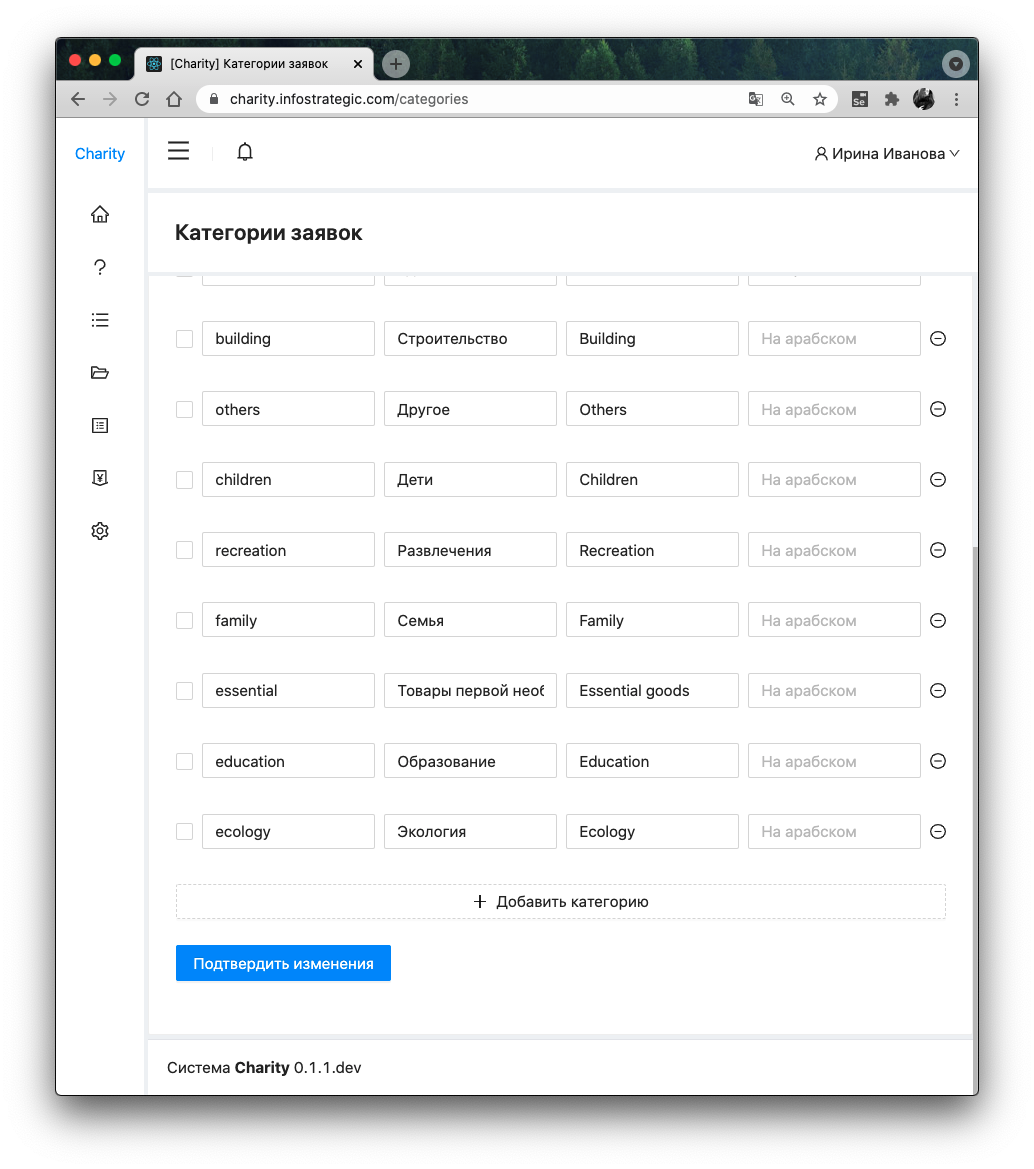
\includegraphics[width=\linewidth]{img/ro/categories.png}
		\end{subfigure}
		\caption{Скриншот просмотра и редактирования категорий}
		\label{pic: categories}
\end{figure}

Рассмотрим подробнее происходящее на диаграмме: сотрудник фонда с ролью <<Член комиссии>> инициирует переход на карточку заявки в статусе <<Ждет подтверждения от члена комисии>>.  Пример UI представлен на скриншотах \ref{pic: vote}: в зависимости от того, соответствует ли назначенная категория члена комисии категории заявки, сотрудник фонда видит либо экран с результатами голосования (слева), либо с результатами и возможностью проголосовать самому (справа).

\begin{figure}[H]
	    \centering
		\begin{subfigure}[b]{0.475\linewidth}
			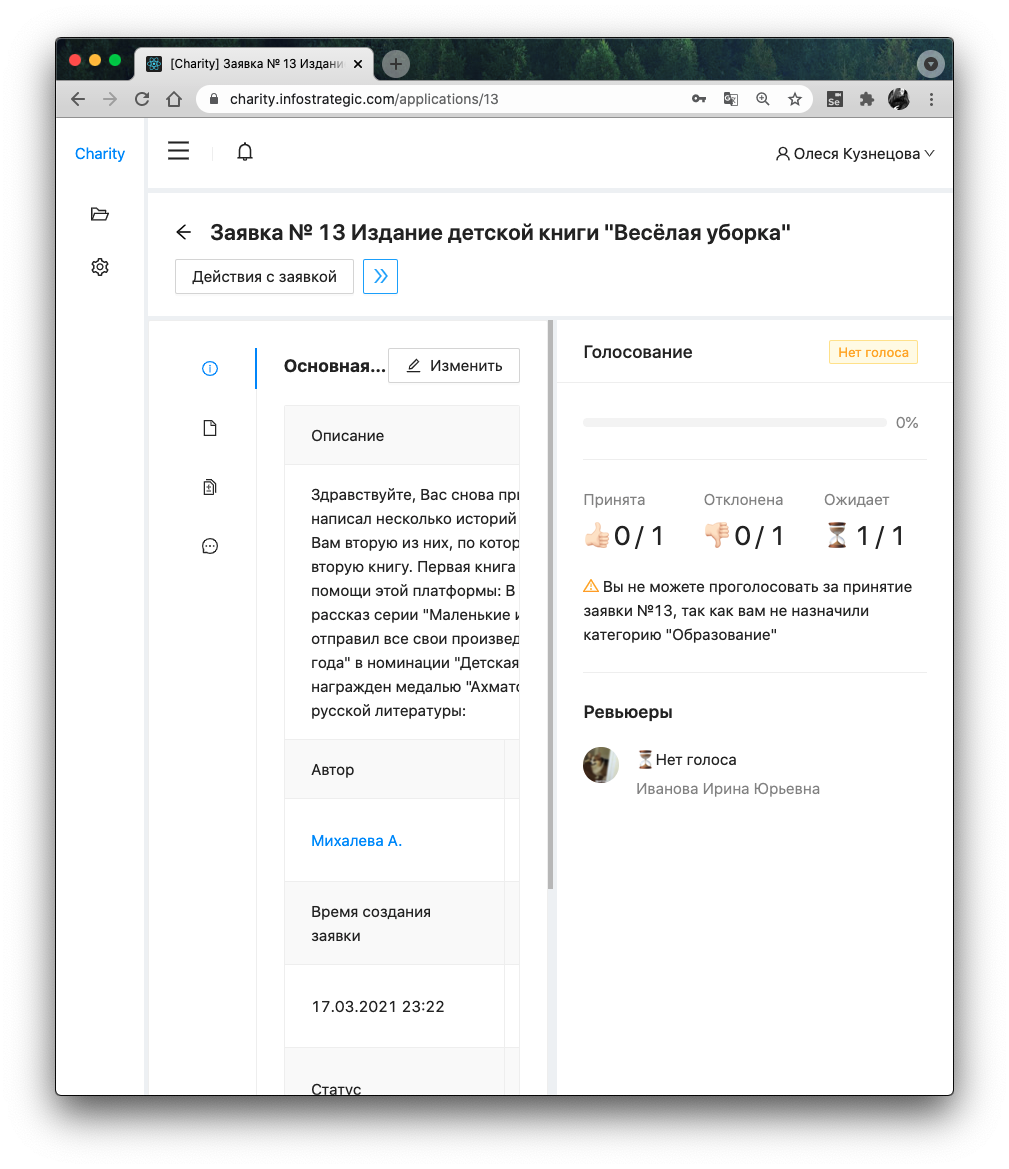
\includegraphics[width=\linewidth]{img/ro/application_m_vote.png}
		\end{subfigure}
		\begin{subfigure}[b]{0.475\linewidth}
			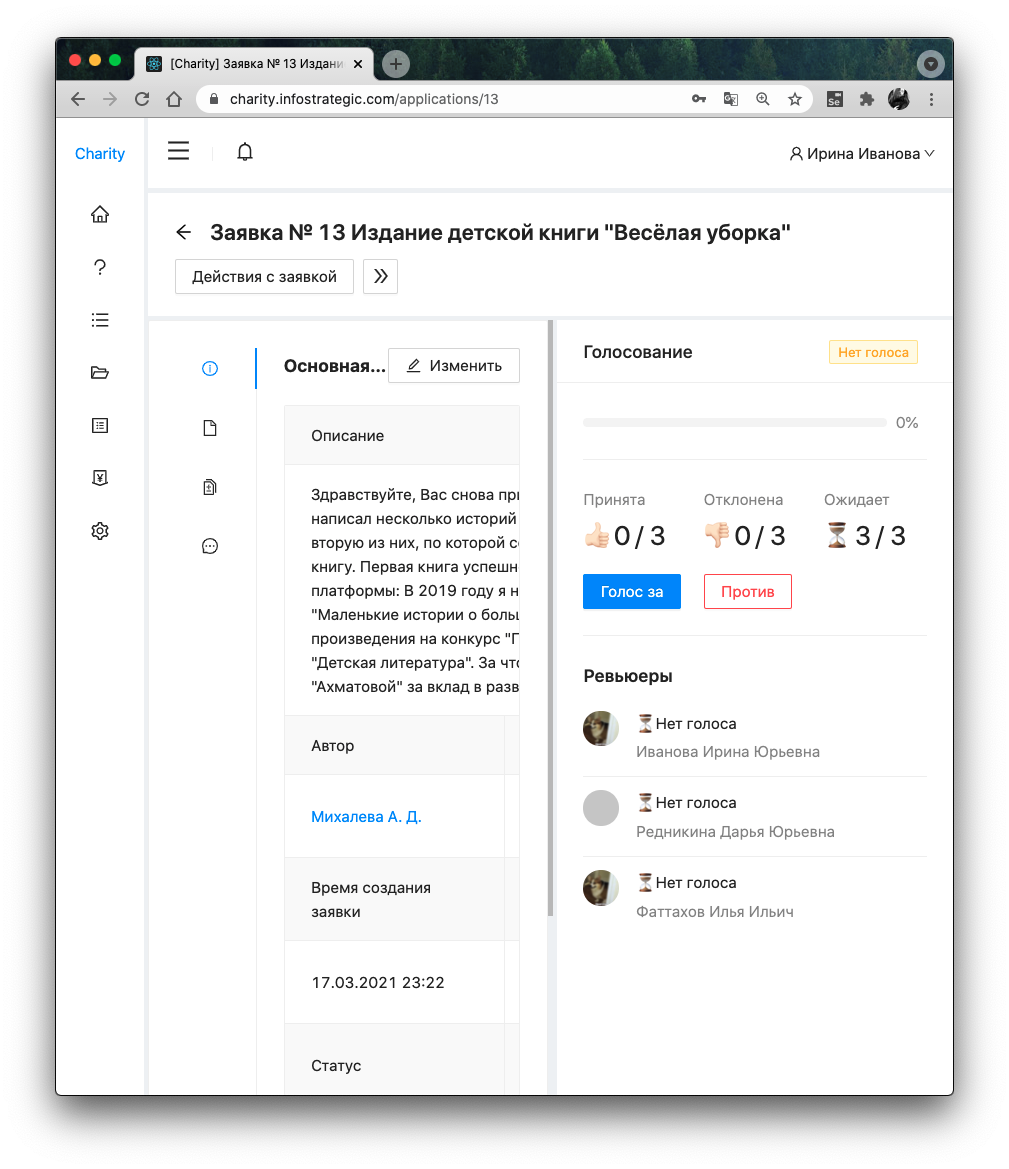
\includegraphics[width=\linewidth]{img/ro/not_voted.png}
		\end{subfigure}
		\caption{Скриншоты голосования за активацию заявки, член комисии}
		\label{pic: vote}
\end{figure}
	
Далее член комисии, который может проголосовать по заявке, совершает свой выбор. Данный выбор фиксируется в API и обновленные данные по голосованию демонстрируются на WebUI. Далее, если все ревьюеры проголосовали и проголосовали положительно, то у члена комиссии появляется возможность изменить статус заявки на <<Ждет активации пользователя>>, тем самым продвинуть ее дальше на активацию. Если же по завершению голосования результаты расходятся, то у члена комисии появляется возможность отклонить заявку, переведя ее в статус <<Отклонена>>. Если же не все ревьюеры успели проголосовать по заявке, то нужно дожидаться пока все проголосуют и дальше будет возможно совершить вышеперечисленные действия. Итогом бизнес-процесса является изменившийся статус заявки. 
	
\begin{figure}[H]
		\centering
		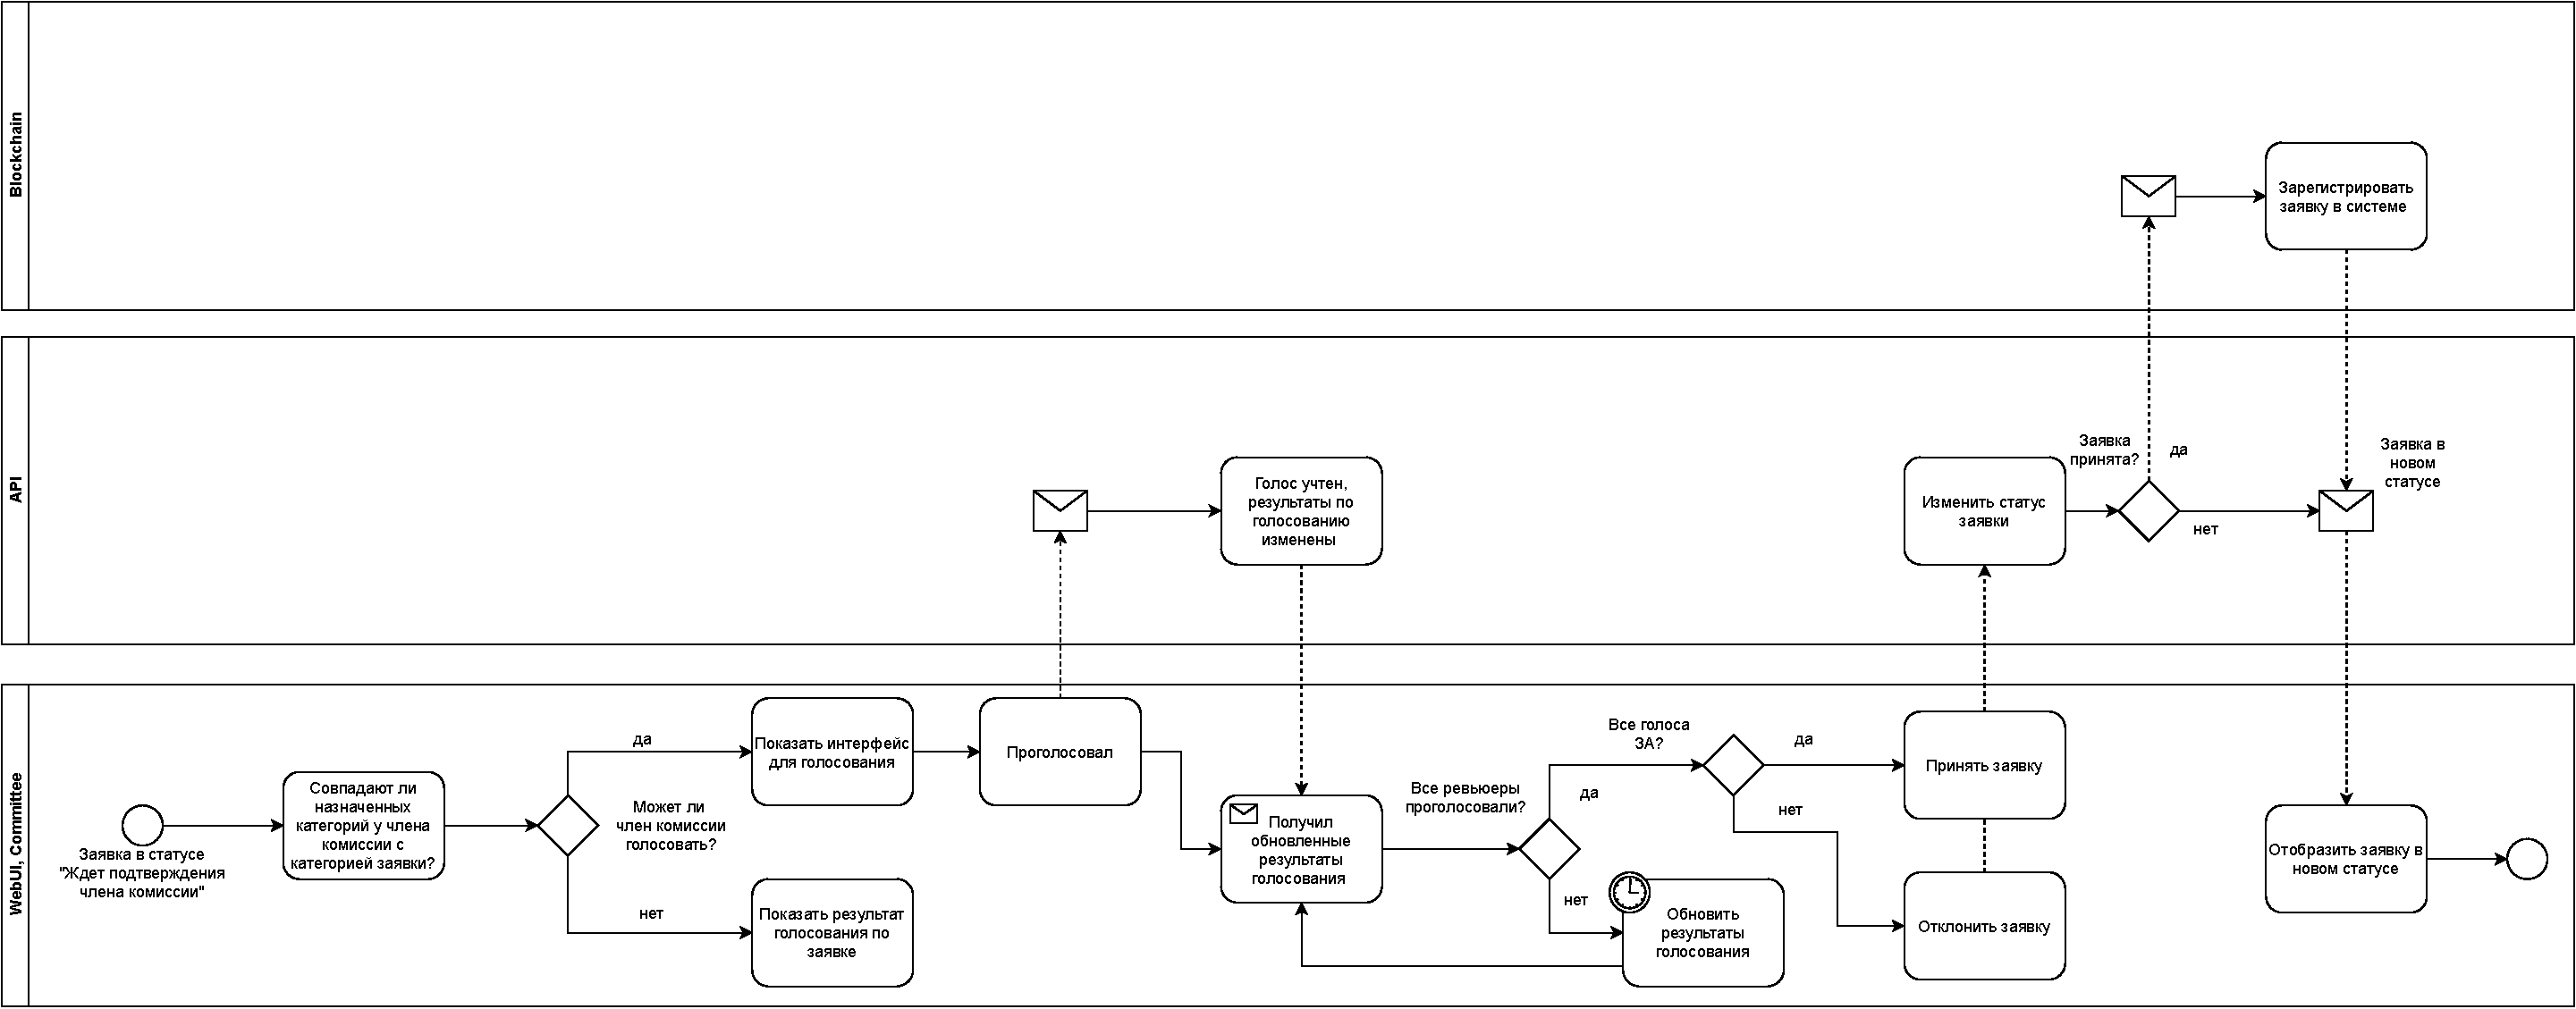
\includegraphics[width = \linewidth]{img/vote_flow.pdf}
		\caption{BPMN голосования по заявке}
		\label{pic: vote_flow}
\end{figure}

\subsection{Процесс получения собранных средств}

Для фонда <<AIAIN>> важным бизнес-процессом является не только сбор средств, но и их перевод. Важно также не только перевести собранные средства на счет нуждающимся, но также и убедиться в законности распределения собранных средств (см. диаграмму \ref{pic: close_bpmn}). 

При моделировании данного бизнес процесса была составлена диаграмма Business Process Model and Notation (BPMN~\cite{bpmn}). Главные участники бизнес процесса: член комиссии (использует Web-интерфейс) и нуждающийся (использует Android-приложение). Второе действующее лицо процесса -- банк, через который происходит передача собранных средств нуждающимся. При реализации данного приложения была опущена реализация интеграции с банковской системы, но для будущего развития проекта были сделаны заглушки для дальнейшей интеграции. 

\begin{figure}[H]
		\centering
		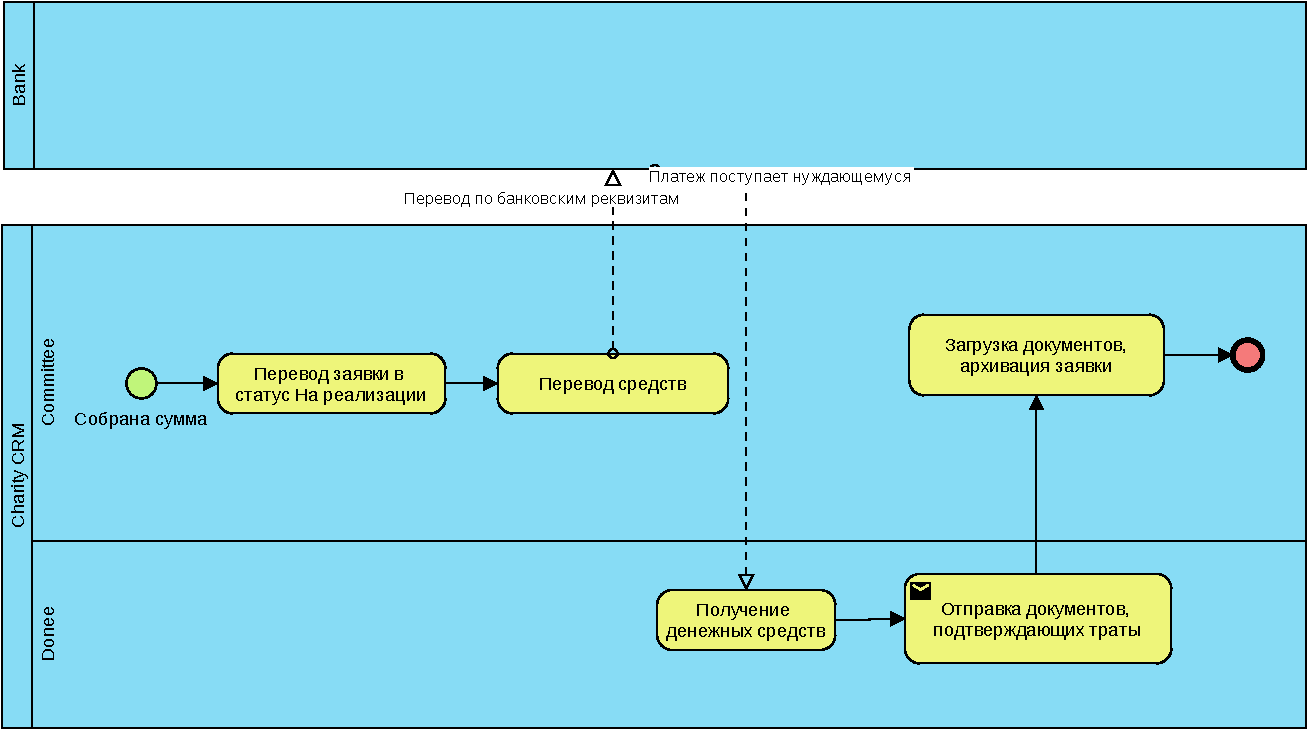
\includegraphics[width = \linewidth]{img/BPMN_close.pdf}
		\caption{BPMN перевода средств нуждающемуся}
		\label{pic: close_bpmn}
\end{figure}

При детальном рассмотрении диаграммы можно увидеть, что бизнес-процесс начинается, когда сумма на заявку собрана (или закончился срок заявки). Член комиссии с помощью Web-приложения переводит заявку в статус <<На реализации>>. Далее собранные средства со счета фонда по банковским реквизитам переводятся нуждающемуся. О потраченных средствах нуждающийся спустя время должен предоставить документы, прислав письмо на почту фонда (или прислав их в чат поддержки). После получения документов уже член комиссии загружает подтверждающие документы и тем самым архивирует заявку, сообщая о ее успешном завершении.

\subsection{Процесс выплаты закята}

При моделировании бизнес процесса сбора средств на выплату закята была составлена диаграмма Business Process Model and Notation (BPMN~\cite{bpmn}), в которой был смоделирован бизнес-процесс и показано, как модули CRM-системы взаимодействуют между собой (см. диаграмму \ref{pic: zakyat_flow}).

Прежде всего стоит отметить, что закят - ежегодный налог в Исламе, собранные средства с которого идут на помощь нуждающимся единоверцам. Одно из главных требований арабского фонда <<AIAIN>> состояло в том, чтобы автоматизировать сбор самого закята и распределение собранных средств между нуждающимимся. 

Первым этапом бизнес-процесса является создание приватной категории <<Закят>>, которая доступна к выбору непосредственно во время создания заявки членом комиссии от имени фонда. Приватные категории, созданные членами комиссии, недоступны для выбора пользователям при создании заявок на сбор пожертвований. 

После создания приватной категории <<Закят>>, член комисии инициирует создание заявки от имени фонда. Заявка, созданная с категорией <<Закят>> может быть создана только по инициативе фонда, таким образом она сразу становится активной, минуя валидацию и подтверждения от членов комисиий. Срок сбора по заявке с категорией <<Закят>> заканчивается, когда наступает Рамадан (определение можно найти в разделе <<Понятия и определения>>). Собранные средства по заявке с категорией <<Закят>> распределяются через форму распределения средств между другими заявками фонда.
	
\begin{figure}[H]
		\centering
		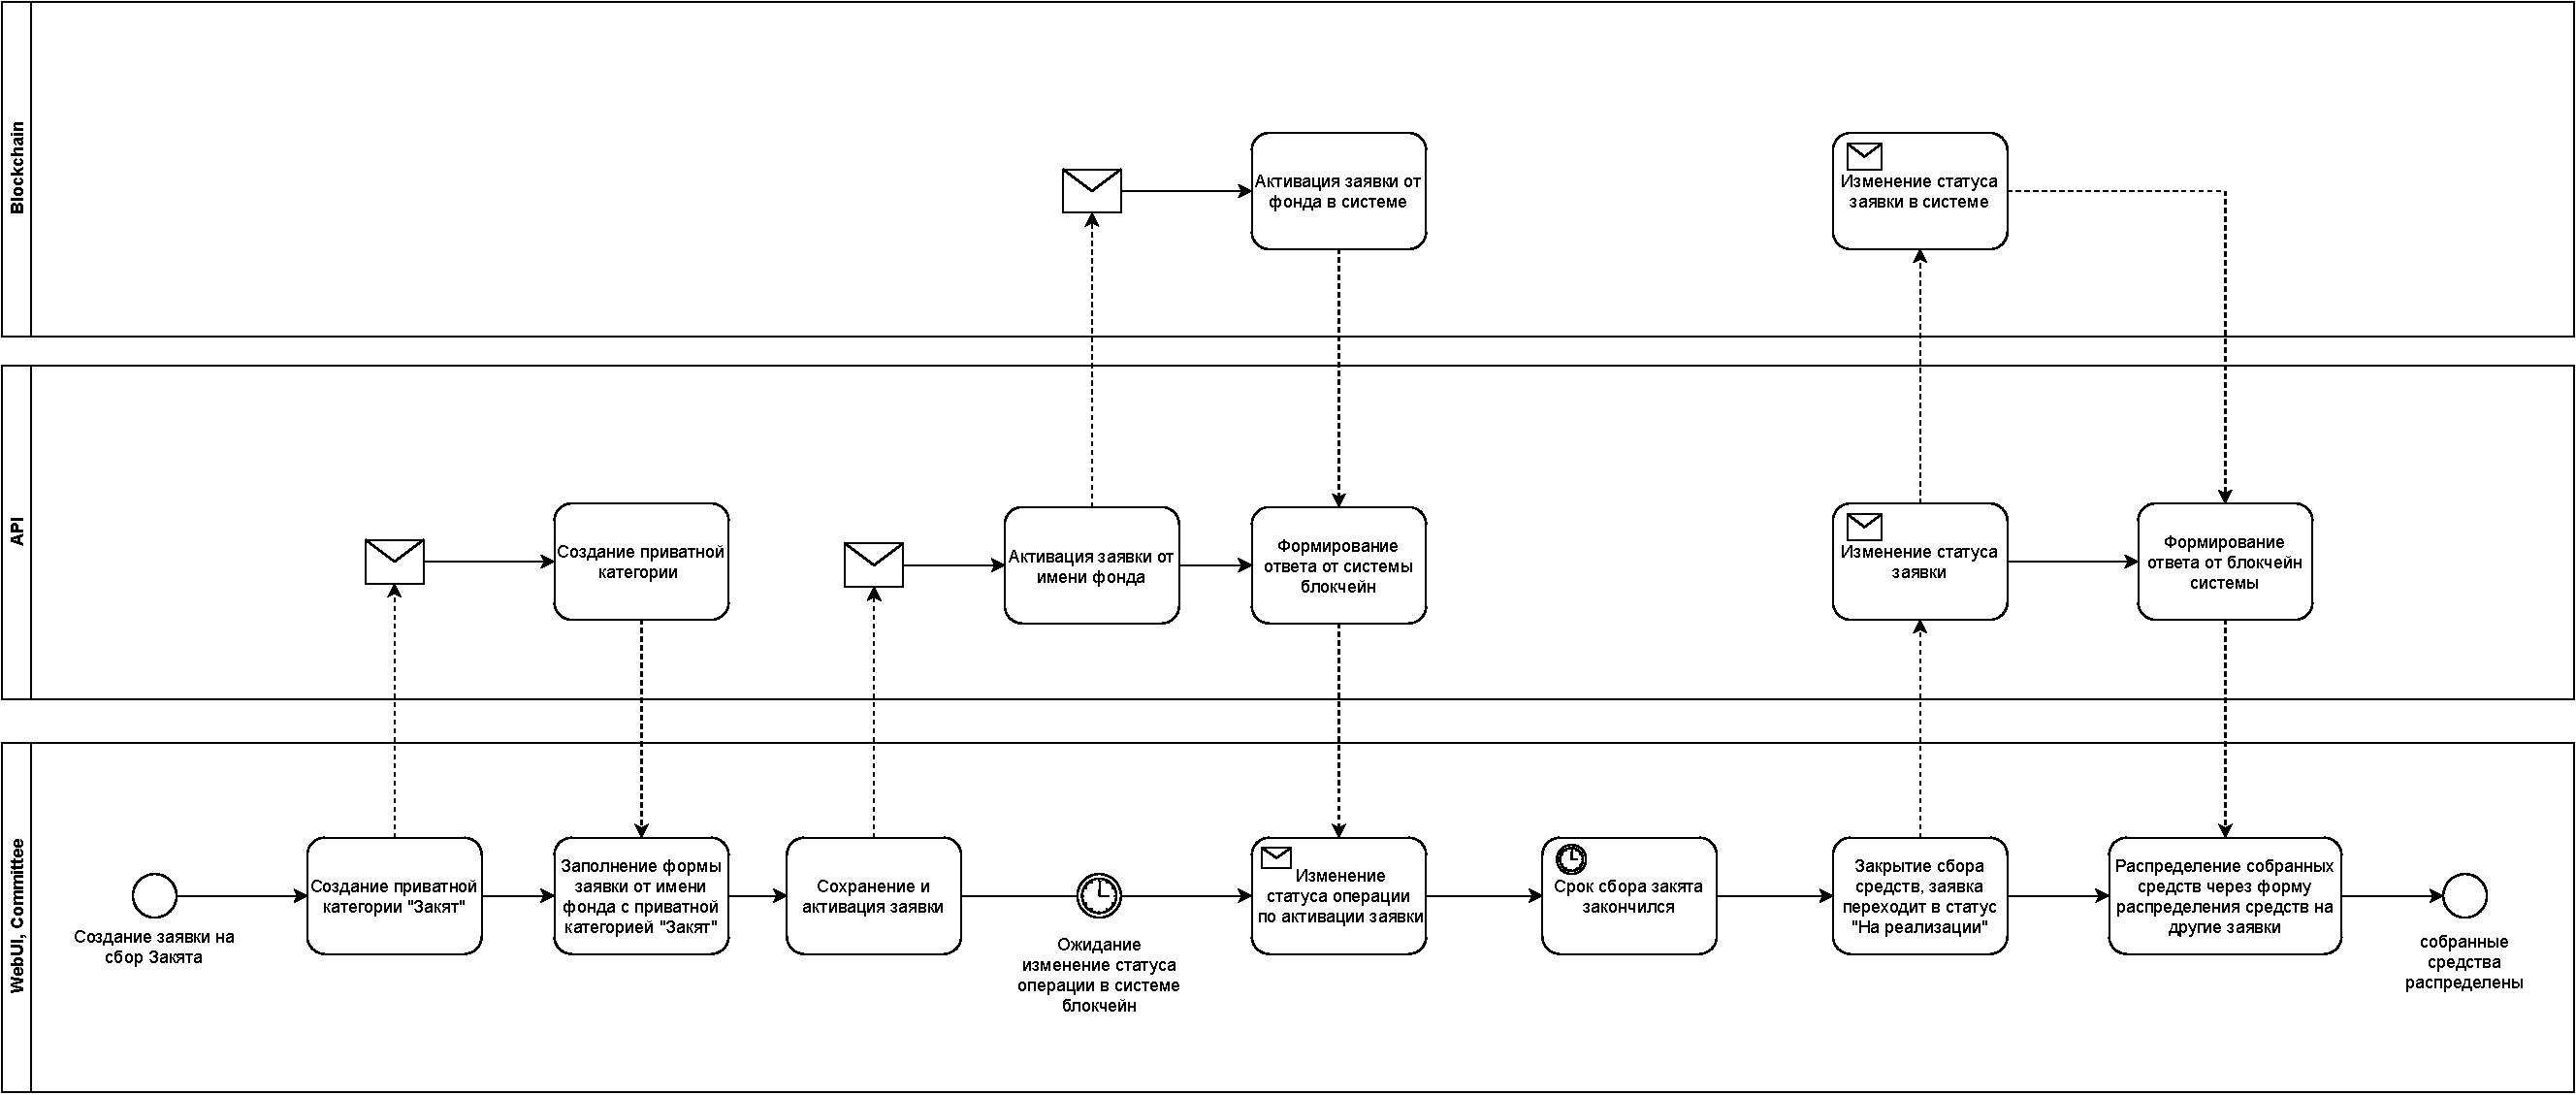
\includegraphics[width = \linewidth]{img/zakyat_flow.pdf}
		\caption{BPMN процесс сбора средств и выплаты закята}
		\label{pic: zakyat_flow}
\end{figure}

\subsection{Ролевая модель} \label{theory-rbac}

Одной из ключевых возможностей приложения является разделение функциональности Web-приложения: только пользователи с определенной ролью могут использовать некоторые функции приложения, а также возможности пользователей с разными ролями могут пересекаться (прим. просмотр заявок у членов комиссии и менеджеров). 

При выборе подхода к проектированию ролевой модели в приложении был выбрана модель \texttt{Role-Based Access Control}~\cite{rbac}. Идея данного похода заключается в хранении прав на совершение действий в зависимости от роли пользователя. При использовании \texttt{RBAC} нужно проанализировать потребности будущих пользователей и сгруппировать их по ролям на основе общих обязанностей. Далее нужно назначить одну или несколько ролей пользователям и соответствующие разрешения для каждой роли. Таким образом не нужно каждый раз рассматривать каждого пользователя отдельно, вместо этого достаточно применить подход разделения <<роль -- привелегия>>.

\subsubsection*{Преимущества подхода}
Преимущества подхода \texttt{RBAC} следующие:

\begin{itemize}
    \item Создание систематического, легко адаптируемого решения с назначением разрешенных действий;
    \item Можно легко добавлять, а также проверять права пользователей;
    \item Легкое и быстрое изменение самих ролей;
    \item Подход дает возможность более эффективно соблюдать нормативные и законодательные требования в отношении конфиденциальности и неприкосновенности частной жизни;
\end{itemize}

\subsubsection*{Роли}

Роли -- это набор разрешений, применяемых к пользователям. Использование ролей упрощает настройку разрешений, специальных функций, доступных узкому кругу лиц. По мере увеличения масштабов и сложности пользовательской базы роли становятся особенно полезными. Так как требования заказчика могут корректироваться, а следовательно и расширяться возможности пользователей, а также появляться новые роли, то этот подход прекрасно позволяет адаптироваться к таким изменениям.


\subsubsection*{Адаптация подхода к приложению}

Что касается разрабатываемого приложения, то как было описано в разделе \ref{sec: listusers}, у каждого пользователя должна быть своя роль и в зависимости от нее - набор функций, доступных для выболнения. 

При разработке аналитической модели приложения была создана неформальная модель будущих пользователей с перечислением функций для каждой из роли в формате словаря. 

\anonsubsection{Выводы по главе}

На данном этапе разработки ПО были получены следующие артефакты: модель прецедентов (см. диаграмму \ref{pic: usecase}) и модель предметной области (см. диаграмму \ref{pic: domain}). Также был детально проработан бизнес-процесс обработки заявки различными пользователями системы (см. диаграмму \ref{pic: status}).   

\newpage

\setcounter{section}{3}
\setcounter{subsection}{0}
\sectionVKR{Проектирование Web-приложения} \label{sec: 3}


\subsection{Выбор технологий} \label{sec: tech}

Разработка Web-приложения началась в ноябре 2020 в рамках предмета <<Командный проект>> ОП <<Программная инженерия>>. Только в марте 2021 года после успешной защиты проекта было принято решение продолжить разработку Web-клиента в качестве дипломной работы. Так как в начале разработки предполагалось, что будущее развитие клиентского приложение будет продолжено членами команды, то выбор пал в сторону стека:  \textit{React}, \textit{Typescript}. При продолжении разработки было принято решение использовать язык \texttt{Elm} для написания отдельных компонентов приложения. 

\subsubsection{Выбор языка разработки} \label{sec:lang}

При выборе языков разработки для сравнения использователись наиболее популярные языки для Web-разработки в 2021 году~\cite{mostpoplang}.

\paragraph*{Сравнение языков для разработки\\}


\textbf{JavaScript} - это высокоуровневый, динамический, нетипизированный интерпретируемый язык программирования. За последние несколько лет JavaScript сохранил свои лидирующие позиции в области разработки корпоративных приложений \cite{webapp}. В таблице \ref{table: lang} сравнения языков для разработки Web-приложений можно выделить главный недостаток Javascript - большое количество ошибок at runtime, отсутствует типизация;

\textbf{Typescript} -- это язык с открытым исходным кодом, который основан на JavaScript, одном из наиболее часто используемых в мире инструментов, путем добавления определений статических типов. Из плюсов (см. Таблицу \ref{table: lang}) стоит выделить большую поддержку языка - все больше и больше приложений с Javascript переписываются на Typescript из-за схожести языков. Но из минусов все те же исключения at runtime, нестрогая типизация. Из преимуществ typescript - он компилируется в Javascript и можно использовать все те же популярные библиотеки, написанные на JavaScript в проекте; 

\textbf{Purescript} -- это чисто функциональный и строго типизированный язык программирования, созданный Филом Фриманом. Он нацелен на обеспечение сильной совместимости с доступными библиотеками JavaScript, по духу схожими с Haskell, но с сохранением JavaScript в своей основе. Сильной стороной PureScript является его минимализм. В нем нет библиотек для функций, которые считались бы необходимыми для других языков. Например, вместо включения генераторов и обещаний в сам компилятор вы можете использовать определенные библиотеки для задачи. Вы можете выбрать желаемую реализацию для нужной вам функции, которая обеспечивает высокоэффективную и персонализированную работу при использовании PureScript, сохраняя при этом сгенерированный код как можно меньше.

\textbf{Elm} -- это чисто функциональный язык программирования, который может компилироваться в JavaScript, HTML и CSS. Вы можете создать полноценный сайт, используя только Elm, что делает его отличной альтернативой фреймворкам JavaScript, таким как React. Приложения, которые создаются с его помощью, автоматически используют виртуальную библиотеку DOM, что делает его очень быстрым. Один большой плюс - это встроенная архитектура, с которой можно забыть о потоке данных и вместо этого сосредоточиться на объявлении данных и логике.

\textbf{CoffeeScript} -- это язык, который нацелен на раскрытие хороших частей JavaScript, обеспечивая при этом более чистый синтаксис и сохраняя семантику на месте. Хотя в последние годы популярность языка снижается, он меняет направление и недавно получил новую основную версию, обеспечивающую поддержку функций ES2015 +. Код, который написан на CoffeeScript, напрямую переводится в читаемый код JavaScript и поддерживает совместимость с существующими библиотеками.

\textbf{Scala} -- этот язык объединяет объектно-ориентированное и функциональное программирование на одном кратком языке высокого уровня. Статические типы Scala помогают избежать ошибок в сложных приложениях, а его среда выполнения JVM и JavaScript позволяет создавать высокопроизводительные системы с легким доступом к огромным экосистемам библиотек.


\label{subsub: lang}

\begin{center}
\begin{longtable}{|p{0.15\linewidth}|p{0.4\linewidth}|p{0.4\linewidth}|}
\caption{Сравнение языков программирования для разработки Web-приложений} 
\label{table: lang} \\

\hline
\multicolumn{1}{|c|}{\textbf{Язык}} & \multicolumn{1}{c|}{\textbf{Плюсы}} & \multicolumn{1}{c|}{\textbf{Минусы}} \\ \hline
\endfirsthead

\multicolumn{3}{r}%
{{ \tablename\ \thetable{} -- продолжение}} \\ 
\hline 
\multicolumn{1}{|c|}{\textbf{Язык}} & \multicolumn{1}{c|}{\textbf{Плюсы}} & \multicolumn{1}{c|}{\textbf{Минусы}} \\ \hline
\endhead

\multicolumn{3}{r}{{Продолжение на следующей странице}} \\ 
\endfoot

\hline 
\endlastfoot

Javascript & Большое коммьюнити; Простота в изучении и написании кода; Совместимость с другими языками; Популярность срези enterprise разработки; Большое количество библиотек и их поддержка сообществом; &  Исключения в процессе исполнения; Нет проверки типов; Нетипизируемый; Недостаток тулинга для дебага приложения;  \\ \hline

Typescript & Аналогичные плюсы JavaScript, а также наличие типов - писать код становится легче и все реже появляются ошибки во время исполнения; & Проверка типов есть, но очень базовая; Недсотаток тулинга для дебага приложения; \\ \hline


Purescript & Функциональный язык программирования; Строгое типизирование; Нет ошибок во время исполнения; & Высокий порог вхождения в язык; Маленькое коммьюнити и библиотек намного меньше и плохо поддерживаются; \\ \hline

Elm & Функциональный язык программирования; Встроенная архитектура model view update, не надо использовать сторонние фреймворки; Никаких исключений во время исполнения; Прекрасная производетельность по сравнению с остальными; & Высокий порог вхождения; По сравнению с js маленькое коммьюнити, а также набор библиотек для UI; \\ \hline

Scala & Совместимость с Java -- можно использовать библиотеки, написанные как на Scala, так и на Java; Функциональная и ОО парадигмы; Строгая типизация; & Фреймворки для UI не такие разнообразные, как для Javascript и Typescript; \\ \hline

\end{longtable}
\end{center}

\paragraph*{Обоснование выбора\\}

Я остановилась на использовании \textbf{Typescript} и \textbf{Elm} для создания Web-приложения. Так как один из плюсов языка Typescript в том, что у языка большая база библиотек, а также можно использовать библиотеки, написанные на языке JavaScript, то было легко найти подходящую библиотеку с готовыми компонентами для реализации UI, а также библиотки для кодогенерации запросов API, реализации переводов и так далее. Более подробно выбор библиотек описан в разделе \ref{sec: libr}. 

Язык Elm привлек своей функциональной парадигмой, встроенной архитектурой и строгой типизацией. Также компоненты на Elm легко встраиваются~\cite{elm-ports} в код, написанный на Typescript и React, поэтому было легко адаптировать компоненты в уже существующий проект.


\subsubsection{Выбор фреймворков}


Так как на момент выбора фреймворка для разработки Web-приложения уже был выбран язык \textit{Typescript} (а в последующем и \textit{Elm}), то список был ограничен фреймворками, которые совместимы с этими языками: React, Angular, Vue, Dojo и другие \cite{ts-frameworks}. Для того, чтобы уменьшить количество потенциальных решений, было принято решение сузить список исходя из метрики распространенности и популярности технологии. Так, в статье-сравнении Web-фреймворков от 2020 года~\cite{realworld} приведена статистика популярности github-репозиториев среди пользователей сообщества. Таким образом полное сравнение следующих Web-фреймворков было проведено: React/Redux, Angular, Vue, Elm.

Для сравнения выбранных фреймворков были выбраны использованы следующие метрики: производительность, размер (самого приложения), количество строк кода, а также развитость сообщества и количество библиотек. Результаты и анализ сравнения производительности, размера и количества строк кода были изучены по статье-сравнению 2020 года~\cite{realworld}. Результаты сравнения можно увидеть на рисунках \ref{assets} и \ref{performance}. Со стороны метрики <<Размер>> наиболее лучшими вариантами являются приложения, написанные с помощью стека Elm и React, в то время как со стороны метрики <<Производительность>> фаворитом является Elm. 

\begin{figure}[H]
		\centering
		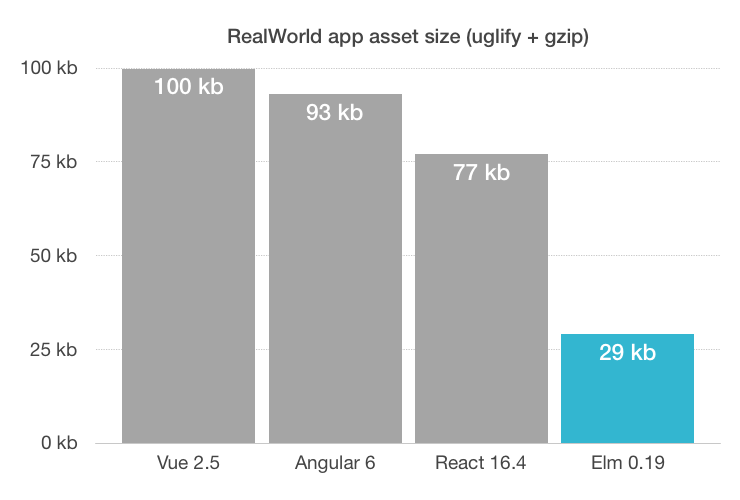
\includegraphics[width = 0.8\linewidth]{img/asset-sizes.png}
		\caption{Сравнение размера app assets \cite{assets}}
		\label{assets}
\end{figure}

\begin{figure}[H]
		\centering
		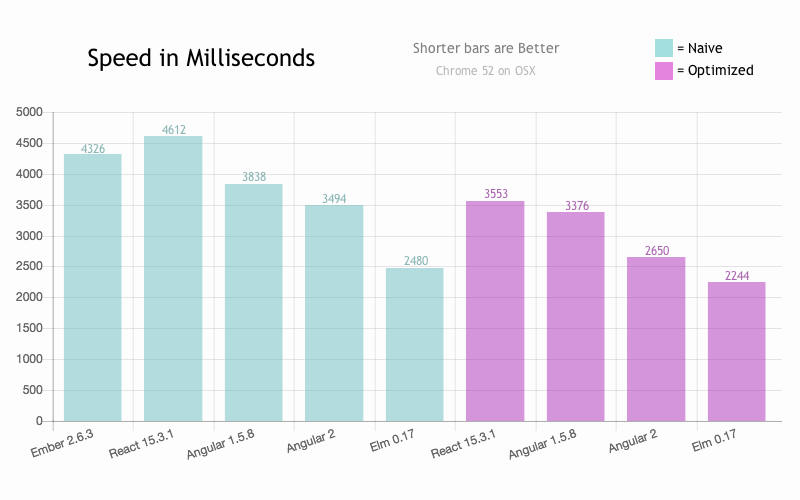
\includegraphics[width = 0.9\linewidth]{img/chrome_speed.png}
		\caption{Сравнение скорости в браузере Google Chrome \cite{performance}}
		\label{performance}
\end{figure}

Также стоит отметить, что стек React/Redux является на данный момент самым популярным среди профессиональных разработчиков~\cite{cool}, соответственно и коммьюнити вокруг стека развито очень хорошо. Об этом свидетельствует большое количество UI-фреймворков для написания React-компонент. 

\paragraph*{Обоснование выбора\\}

Для написания приложения на языке \textit{Elm} не нужен сторонний фреймворк, поэтому для написания основной части на языке \textit{Typescript} был выбран фреймворк \textit{React}, как наиболее подходящий под цели разработки. Большое профессиональное коммьюнити и широкий выбор библиотек позволят использовать все удобства и возможности Web-разработки, а хорошие показатели в метриках <<Размер>> и <<Производительность>> прекрасно характеризуют выбранный стек.

\subsubsection{Выбор библиотек} \label{sec: libr}

Выбор библиотек для приложения состоял из двух этапов: изначально для части приложения, написанного на стеке React, Typescript, Redux были выбраны зависимости; позже при написании части кода на Elm были выбраны зависимости для этого стека, а также были подобраны зависимости для связывания частей, написанных на Elm и React, вместе.

\paragraph*{React\\}

Так как разрабатываемое приложение является клиент-серверным, то в первую же очередь были выбраны библиотеки, позволяющие взаимодействовать с API. Для отправки HTTP запросов выбор происходил между двумя вариантами: встроенным API для создания HTTP-запросов \textit{fetch} и \textit{axios}. Библиотеки отличаются деталями реализации, а также API, но в целом функции выполняют одни и те же. Ключевым моментом в выборе библиотеки для совершения API запросов была возможность кодогенерации кода запросов из swagger схемы (и дальнейшая совместимость сгенерированного когда с библиотекой). Таким образом выбор пал на библиотеку \textbf{Axios}~\cite{axios}. Ниже будем рассматривать вопрос с кодогенерацией кода.

Для кодогенерации кода запросов выбор библиотеки состоял из двух вариантов: \textit{OpenAPI Generator} и \textit{Swagger Codegen}. При сравнении обеих библиотек в первую очередь учитывались языки и фреймворки, с которыми они совместимы: обе поддерживают связку \textit{Typescript} и ранее упомянутый \textit{Axios}. Если рассматривать кодогенераторы более подробно, то можно увидеть, что Swagger Codegen является продуктом SmartBear, в то время как OpenAPI generator - это продукт, которым управляет само сообщество программистов. Более того, активность в репозитории OpenAPI generator
выше, чем в Swagger Codegen. Таким образом выбор все-таки был в пользу \textbf{OpenAPI generator}~\cite{openapi}. Для проекта был написан yarn скрипт, который по находящейся в корне проекта Swagger спецификации в формате json генерирует файлы с методами/моделями для совершения запросов по описанному API.

При выборе библиотеки для дизайна компонент были важны следующие аспекты: поддержка коммьюнити, эстетичность, применимость компонент под цели и задачи проекта. Так как CRM-система предполагает панели для администрирования, поддержку большого количества реестров, фильтрации внутри реестров, расширенного поиска информации -- это накладывает определенные ограничения на существущие библиотеки компонент. При выборе библиотеки были рассмотрены следующие варианты: \textit{Ant.design}, \textit{MaterialUI}, \textit{SemanticUI}. Последние два варианта по набору компонент подходят больше для создания коммерческих сайтов, площадок для тороговли, в отличие от первого варианта. \textbf{Ant.design} был выбран, так как API позволяет настраивать компоненты под себя и прописывать собственную логику в поведение, к тому же UI подходит под цели и здачи проекта. По такому же принципу были выбраны библиотеки для визуализации аналитических дашбордов и диаграмм \textbf{Ant Design Charts}.

Одним из важнейших решений в выборе библиотек для рабзработки была библиотека для интернализации приложения. В одном из требований заказчика (см. Приложение \ref{additiontz}) в Web-приложени должна быть поддержка двух языков: русский и английский. При реализации механизма интернализации была выбрана библиотека \textbf{i18n} как самая популярная среди разработчиков React приложений. Библиотека поддерживает переводы множественных значений, а также имеет удобное и настраиваемое API.  

Также было принято решение использовать встроенную библиотеку \textbf{WebSocket} для использования в чатах и диалогах для мнгновенного получения входящих сообщений. При выборе была также рассмотрена библиотека \textit{Socket.IO}, которая является надстройкой над \textit{WebSocket}, которая к тому же поддерживает функционал по поллингу и автоматическому реконнекту, если вдруг соединение прервется. Так как базовый функционал встроенной библиотеки \textit{WebSocket} удовлетворяет потребностям проекта, то выбор был остановлен на ней.

Для получения пуш-уведомлений в проекте была использована библиотека \textbf{Firebase}, так как именно с помощью этой технологии бэкенд отправляет пуш-уведомления как на Web-клиент, так и на Android-клиент. 

\paragraph*{Elm\\}

При выборе библиотек для разработки части приложения, написанной на стеке \textit{Elm} помимо стандартных библиотек для http запросов были использованы следующие библиотеки:
\begin{itemize}
    \item elm-explorations/markdown - для отображения  markdown\cite{md} в компоненте;
    \item mdgriffith/elm-ui - для динамической работы с css внутри Elm кода;
    \item webbhuset/elm-json-decode - для синтаксического сахара;
\end{itemize}

Для совместимости кода, написанного на Elm с кодом Typescript также использовалась библиотека \textbf{react-elm-components}, так как она поддерживает функциональность флагов и портов~\cite{elm-ports} в отличие от остальных существующих решений.


\subsection{Архитектура приложения}

В начале разработки клиентского Web-приложения была выбрана архитектура Single Page Application, далее SPA~\cite{spa}. 

Главное преимущество выбора данной архитектуры - потрясающий пользовательский интерфейс, поскольку пользователи не ждут перезагрузки веб-страниц. Таким образом это позволяет пользователям использовать приложения, не дожидаясь загрузки страницы с сервера, что позволяет выиграть в производительности и более динамическом пользовательском опыте. Однако существуют и минусы у данной архитектуры - требуется больше усилий для поддержания состояния данных на странице, реализации навигации и значительного мониторинга производительности. 

При выборе SPA архитектуры большое внимание было уделено выбору роутера (библиотеки для навигации между страницами Web-приложения). При детальном рассмотрении существующих решений было выделено два подхода к реализации межстраничной навигации:

\begin{itemize}
    \item Большинство маршрутизатором для SPA используют синхронный роутинг для подгрузки страницы. Это означает, что изменение местоположение происходит до сопоставления роута. Порядок действий примерно такой: пользователь нажимает на ссылку, изменяется ссылка в url браузера, роутер находит подходящий переход и происходит новый рендеринг страницы;
    \item Асинхронный роутинг подразумевает что url не меняется до самого последнего момента: пока другие асинхронные действия не будут завершены (например загрузка данных). Порядок действий примерно такой: пользователь нажимает на ссылку, роутер определяет по какому url будет переход, если у данного перехода есть асинхронные действия, то они отрабатывают, только потом происходит рендер страницы;
\end{itemize}

Был выбран асинхронный роутинг для данного приложения, так как практически на каждой странице происходит асинхронная загрузка данных. Для реализации данного подхода был выбран CuriRouter~\cite{curi} как самое лучшее решение для имплементации асинхронного роутера в React приложениях.

\subsection{Клиент-серверное взаимодействие}

При разработке Web-клиента для CRM-системы для благотворительного фонда <<AIAIN>> большое внимание уделялось клиент-серверному взаимодействию. На раннем этапе разработки системы было принято решение использовать архитектурный стиль REST~\cite{rest} для взаимодействия компонентов между собой. В отличие от рассматриваемых вариантов (прим. GraphQL) REST является самым распространенным архитектурным стилем, а также прекрасно подходит для клиент-серверных приложений. Еще одно удобство использования данного подхода заключается в том, что для REST-запросов легко писать документацию. 

Также в начале разработки было принято решение писать Swagger документацию к endpoint-ам API~\cite{api}, так как она хорошо читаема и с помощью таких сервисов как SwaggerHub~\cite{swaggerhub} ее можно визуализировать. Также, как было упомянуто ранее в разделе \ref{sec: libr}, при проектировании Web-клиента был использован генератор кода API запросов по Swagger документации OpenapiGenerator~\cite{openapi} (см. диаграммы \ref{pic: swagger}). 

При выполнении команды по кодогенерации в папке проекта \texttt{@generated} образовывалась следующая структура, в которой содержались пакет \texttt{api} с файлами запросов, сгруппированных по тематике, а также пакет \texttt{model} с многочисленными моделями, использующимися в самих запросах (см. скриншоты структуры проекта \ref{pic: generated}).  

Для иллюстрации взаимодействия API и Web-клиента приведем пример JSON ответа на запрос получения GET запроса новости фонда (см. листинг \ref{lst:apiex}).
\begin{lstlisting}[frame=single, basicstyle=\footnotesize\ttfamily, label={lst:apiex}, caption={Пример JSON body ответа на запрос GET /api/news/:id},captionpos=b]
{
  created_at: "2021-05-20T17:13:00.391224Z"
  description: "Presented review"
  id: "22249e15-3161-493e-a970-c28d353837e8"
  image_id: "0a53f26bab39e6ff8c3a408f9ba681531447f16b814125f893bed954b"
  text: "Full march report"
  title: "March report"
  updated_at: "2021-05-20T17:13:00.39144Z"
}
\end{lstlisting}

\begin{figure}[H]
	    \centering
		\begin{subfigure}[b]{0.475\linewidth}
			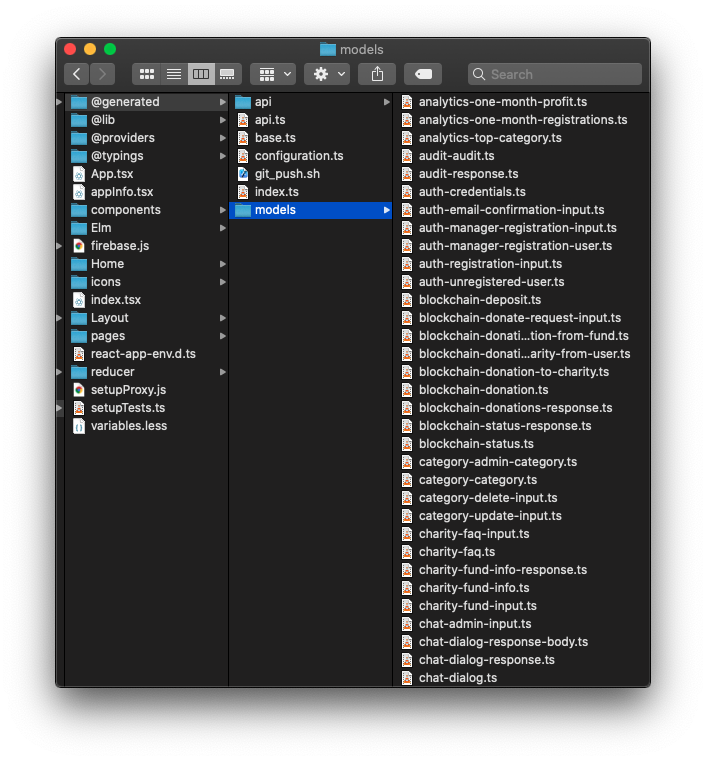
\includegraphics[width=\linewidth]{img/generated1.png}
		\end{subfigure}
		\begin{subfigure}[b]{0.475\linewidth}
			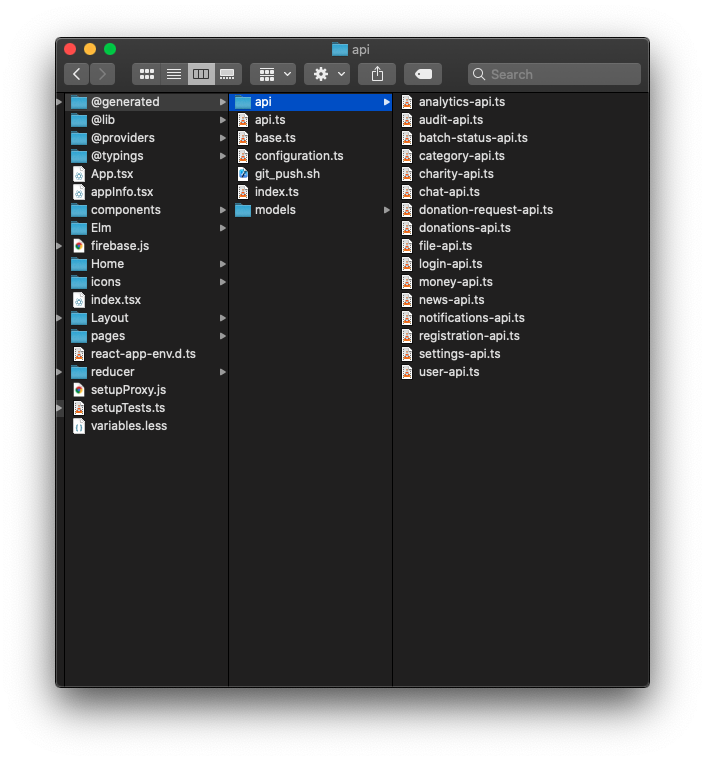
\includegraphics[width=\linewidth]{img/generated2.png}
		\end{subfigure}
		\caption{Скриншоты папки сгенерированного кода запросов}
		\label{pic: generated}
\end{figure}

\begin{figure}[H]
	    \centering
		\begin{subfigure}[b]{0.475\linewidth}
			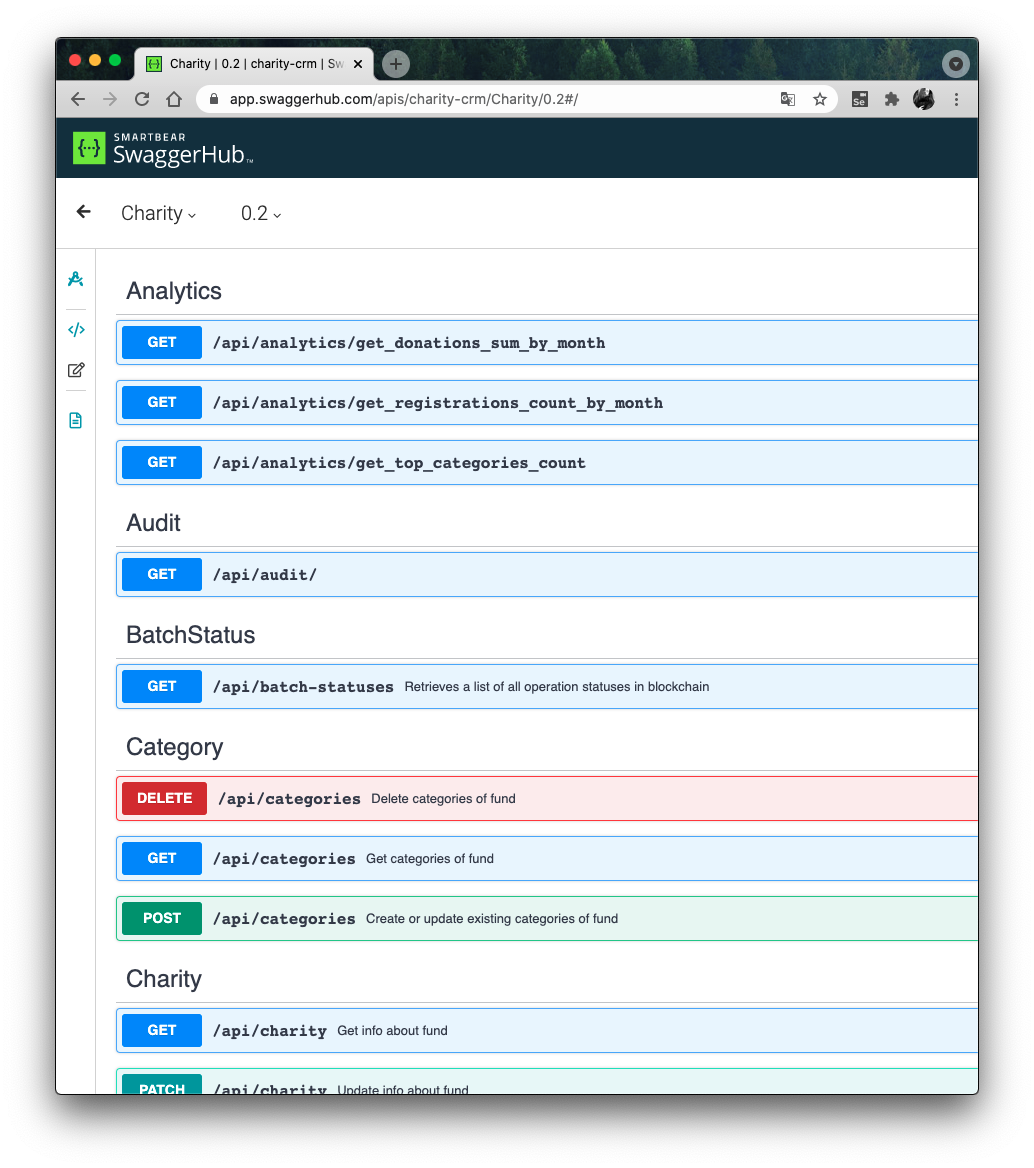
\includegraphics[width=\linewidth]{img/swaggerhub.png}
		\end{subfigure}
		\begin{subfigure}[b]{0.475\linewidth}
			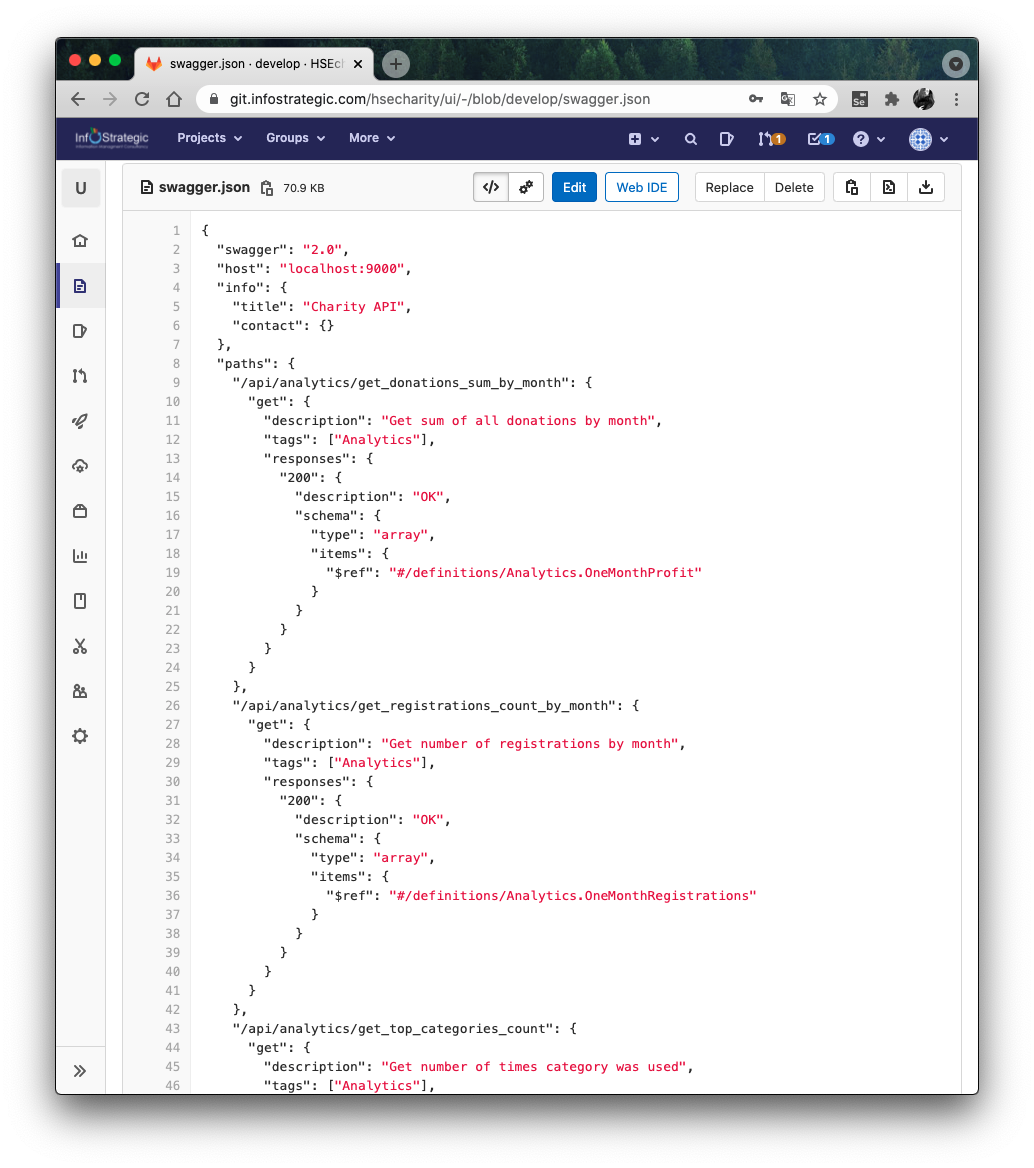
\includegraphics[width=\linewidth]{img/swaggerjson.png}
		\end{subfigure}
		\caption{Скриншоты документации Swagger}
		\label{pic: swagger}
\end{figure}

Одной из важных особенностей взаимодействия с API~\cite{api} является обработка статус-кодов ответа от сервера. При проектировании Web-приложении была составлена таблица со всеми возможными статус-кодами от сервера и их значениями. Данная таблица (см. таблицу \ref{table: codes}) использовалась при обработке ответов от сервера.

\label{subsub: userlist}

\begin{center}
\begin{longtable}{|p{0.2\linewidth}|p{0.35\linewidth}|p{0.4\linewidth}|}
\caption{Статус-коды ответов от сервера} 
\label{table: userlist} \\

\hline
\multicolumn{1}{|c|}{\textbf{Код}} & \multicolumn{1}{c|}{\textbf{Описание}} & \multicolumn{1}{c|}{\textbf{Обработка}} \\ \hline
\endfirsthead

\multicolumn{3}{r}%
{{ \tablename\ \thetable{} -- продолжение}} \\ 
\hline 
\multicolumn{1}{|c|}{\textbf{Код}} & \multicolumn{1}{c|}{\textbf{Описание}} & \multicolumn{1}{c|}{\textbf{Обработка}} \\
\hline
\endhead

\multicolumn{3}{r}{{Продолжение на следующей странице}} \\ 
\endfoot

\hline 
\endlastfoot
\label{table: codes}
200 & Успешный ответ  & В случае успешного ответа обрабатываем полученное тело ответа и демонстрируем его в UI \\ \hline
400 & Плохие входные данные  & В случае некорректного введенного и отправленного значения высвечивается уведомление на UI \\ \hline

401 & Пользователь не авторизован & В случае получения данной ошибки пользователь не авторизован, либо закончился срок действия авторизационного токена. Либо отображается страница с авторизационной формой, либо перезапрашивается авторизационный токен через эндпойнт \texttt{refresh} \\ \hline

403 & Недостаточно прав доступа & В случае получения данной ошибки пользователь перешел на url, к которому у него нет доступа. В данном случае высвечивается соответствующая ошибка в виде уведомления в UI \\ \hline
404 & Запрашиваемый контент не найден & В случае получения данной ошибки либо url запроса некорретный, либо в базе данных не найдена сущность по указанным в запросе параметрам. В данной ситуации обработка подразумевает демонстрацию ошибки на UI \\ \hline

500 & Ошибка сервера & Данная ошибка демонстрируется в виде нотификации на UI \\ \hline


\end{longtable}
\end{center}

\subsection{Дизайн модель}

При проектировании дизайн модели Web-приложения были использованы стандарты UML~\cite{uml}. 

На этапе проектирования была разработана дизайн модель, отражающая разбиение архитектуры приложения на слои. Слоистая архитектура - очень распространенный паттерн при проектировании клиент-серверных приложений, так как слой в слой бизнес-логики можно вывести клиент-серверное взаимодействие, тем самым не затрагивая слой UI компонент (см. диаграмму \ref{pic: designmodel}).

Рассмотрим подробней содержание и взаимодействие слоев Web-приложения. 

\begin{itemize}
    \item UI -- слой с компонентами интерфейса, содержит в себе следующие подсистемы: Login (компоненты для авторизации), Transaction (компоненты, использующиеся на эранах пожертвований), Application (компоненты, использующиеся на эранах заявок), Fund (компоненты, использующиеся на эранах информации о фонде), Settings (компоненты, использующиеся на эранах личного профиля), Manager (компоненты, использующиеся на эранах инорфмации о менеджерах) и т.д; Также в подсистемы слоя интерфейса входили такие подсистемы как Layout и Elm. В Layout содержатся пакеты с макетом общих частей всех экранов приложений (заголовок, футтер, навигационная панель), в Elm подсистеме содержатся компоненты, реализованные на языке Elm с помощью одноименной архитектуры;
    \item BusinessLogic -- слой с бизнес логикой взаимодействия с API; также этот слой содержит бизнес логику, ответственную за переходы статусов и отрисовку соответствующих компонент; в данном слое содержится также подсистема по управлению Role Based Access Controll~\cite{rbac}, т.е ролями пользователей приложения;
    \item Frameworks -- данный слой подробно описан в разделе \ref{sec: libr};
\end{itemize}

\begin{figure}[H]
		\centering
		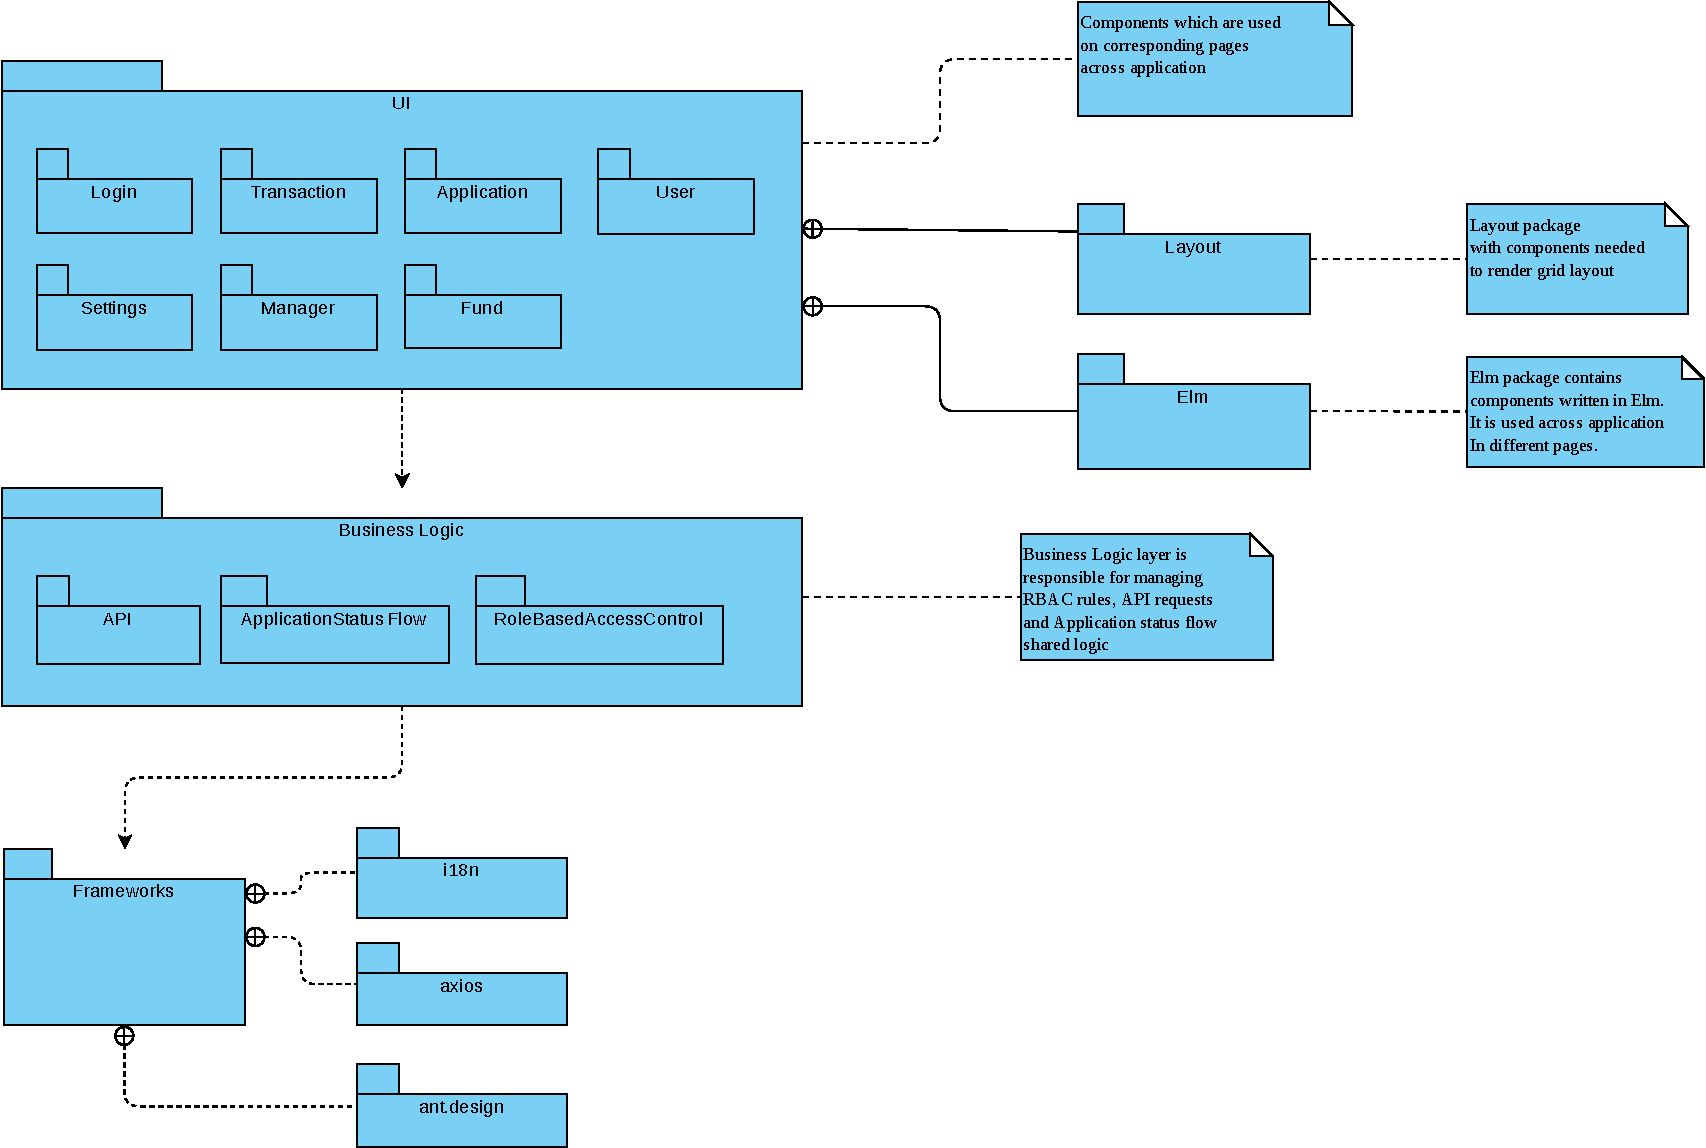
\includegraphics[width = 0.9\linewidth]{img/design model.pdf}
		\caption{Дизайн модель}
		\label{pic: designmodel}
\end{figure}

\subsection{Диаграмма компонентов}

При проектировании диаграммы компонентов Web-приложения были использованы стандарты UML~\cite{uml}. 

Так как диаграмма компонентов показывает разбиение программной системы на структурные компоненты и связи (зависимости) между компонентами, то в качестве физических компонентов были выбраны пакеты, содержащие файлы с расширением \texttt{tsx} и \texttt{elm}. Рассмотрим каждый слой диаграммы, изображенной на рисунке \ref{pic: component}, подробнее.

Как уже было упомянуто в разделе \ref{sec: libr}, при разработке сервиса для отправки API запросов использовалась библиотека для кодогенерации OpenAPI Generator~\cite{openapi} по схеме API Swagger~\cite{api}. Таким образом все интерфейсы и модели в пакете API соответствуют спецификации API запросов. Далее на диаграмме \ref{pic: component} можно увидеть слой \texttt{Components}, состоящий из многочисленных подпакетов с компонентами, а также содержащий две подсистемы \texttt{Layout} и \texttt{Elm}. Первая подсистема ответственна за структурное расположения UI элементов каждой страницы приложения: в ней содержится логика по управлению хэдером, футтером, а также левым навигационным меню, присутствующим на каждой странице приложения. Вторая подсистема - Elm - содержит пакеты с компонентами, написанными на языке Elm. При рассмотрении последнего слоя диаграммы компонентов \texttt{pages} можно увидеть, что каждый подпакет слоя соответствует отдельной web странице, которая отрисовывается на UI при переходе по заданному url. Этот слой активно использует компоненты из слоя \texttt{Components}, а также API запросы из слоя \texttt{API}. 

\begin{figure}[H]
		\centering
		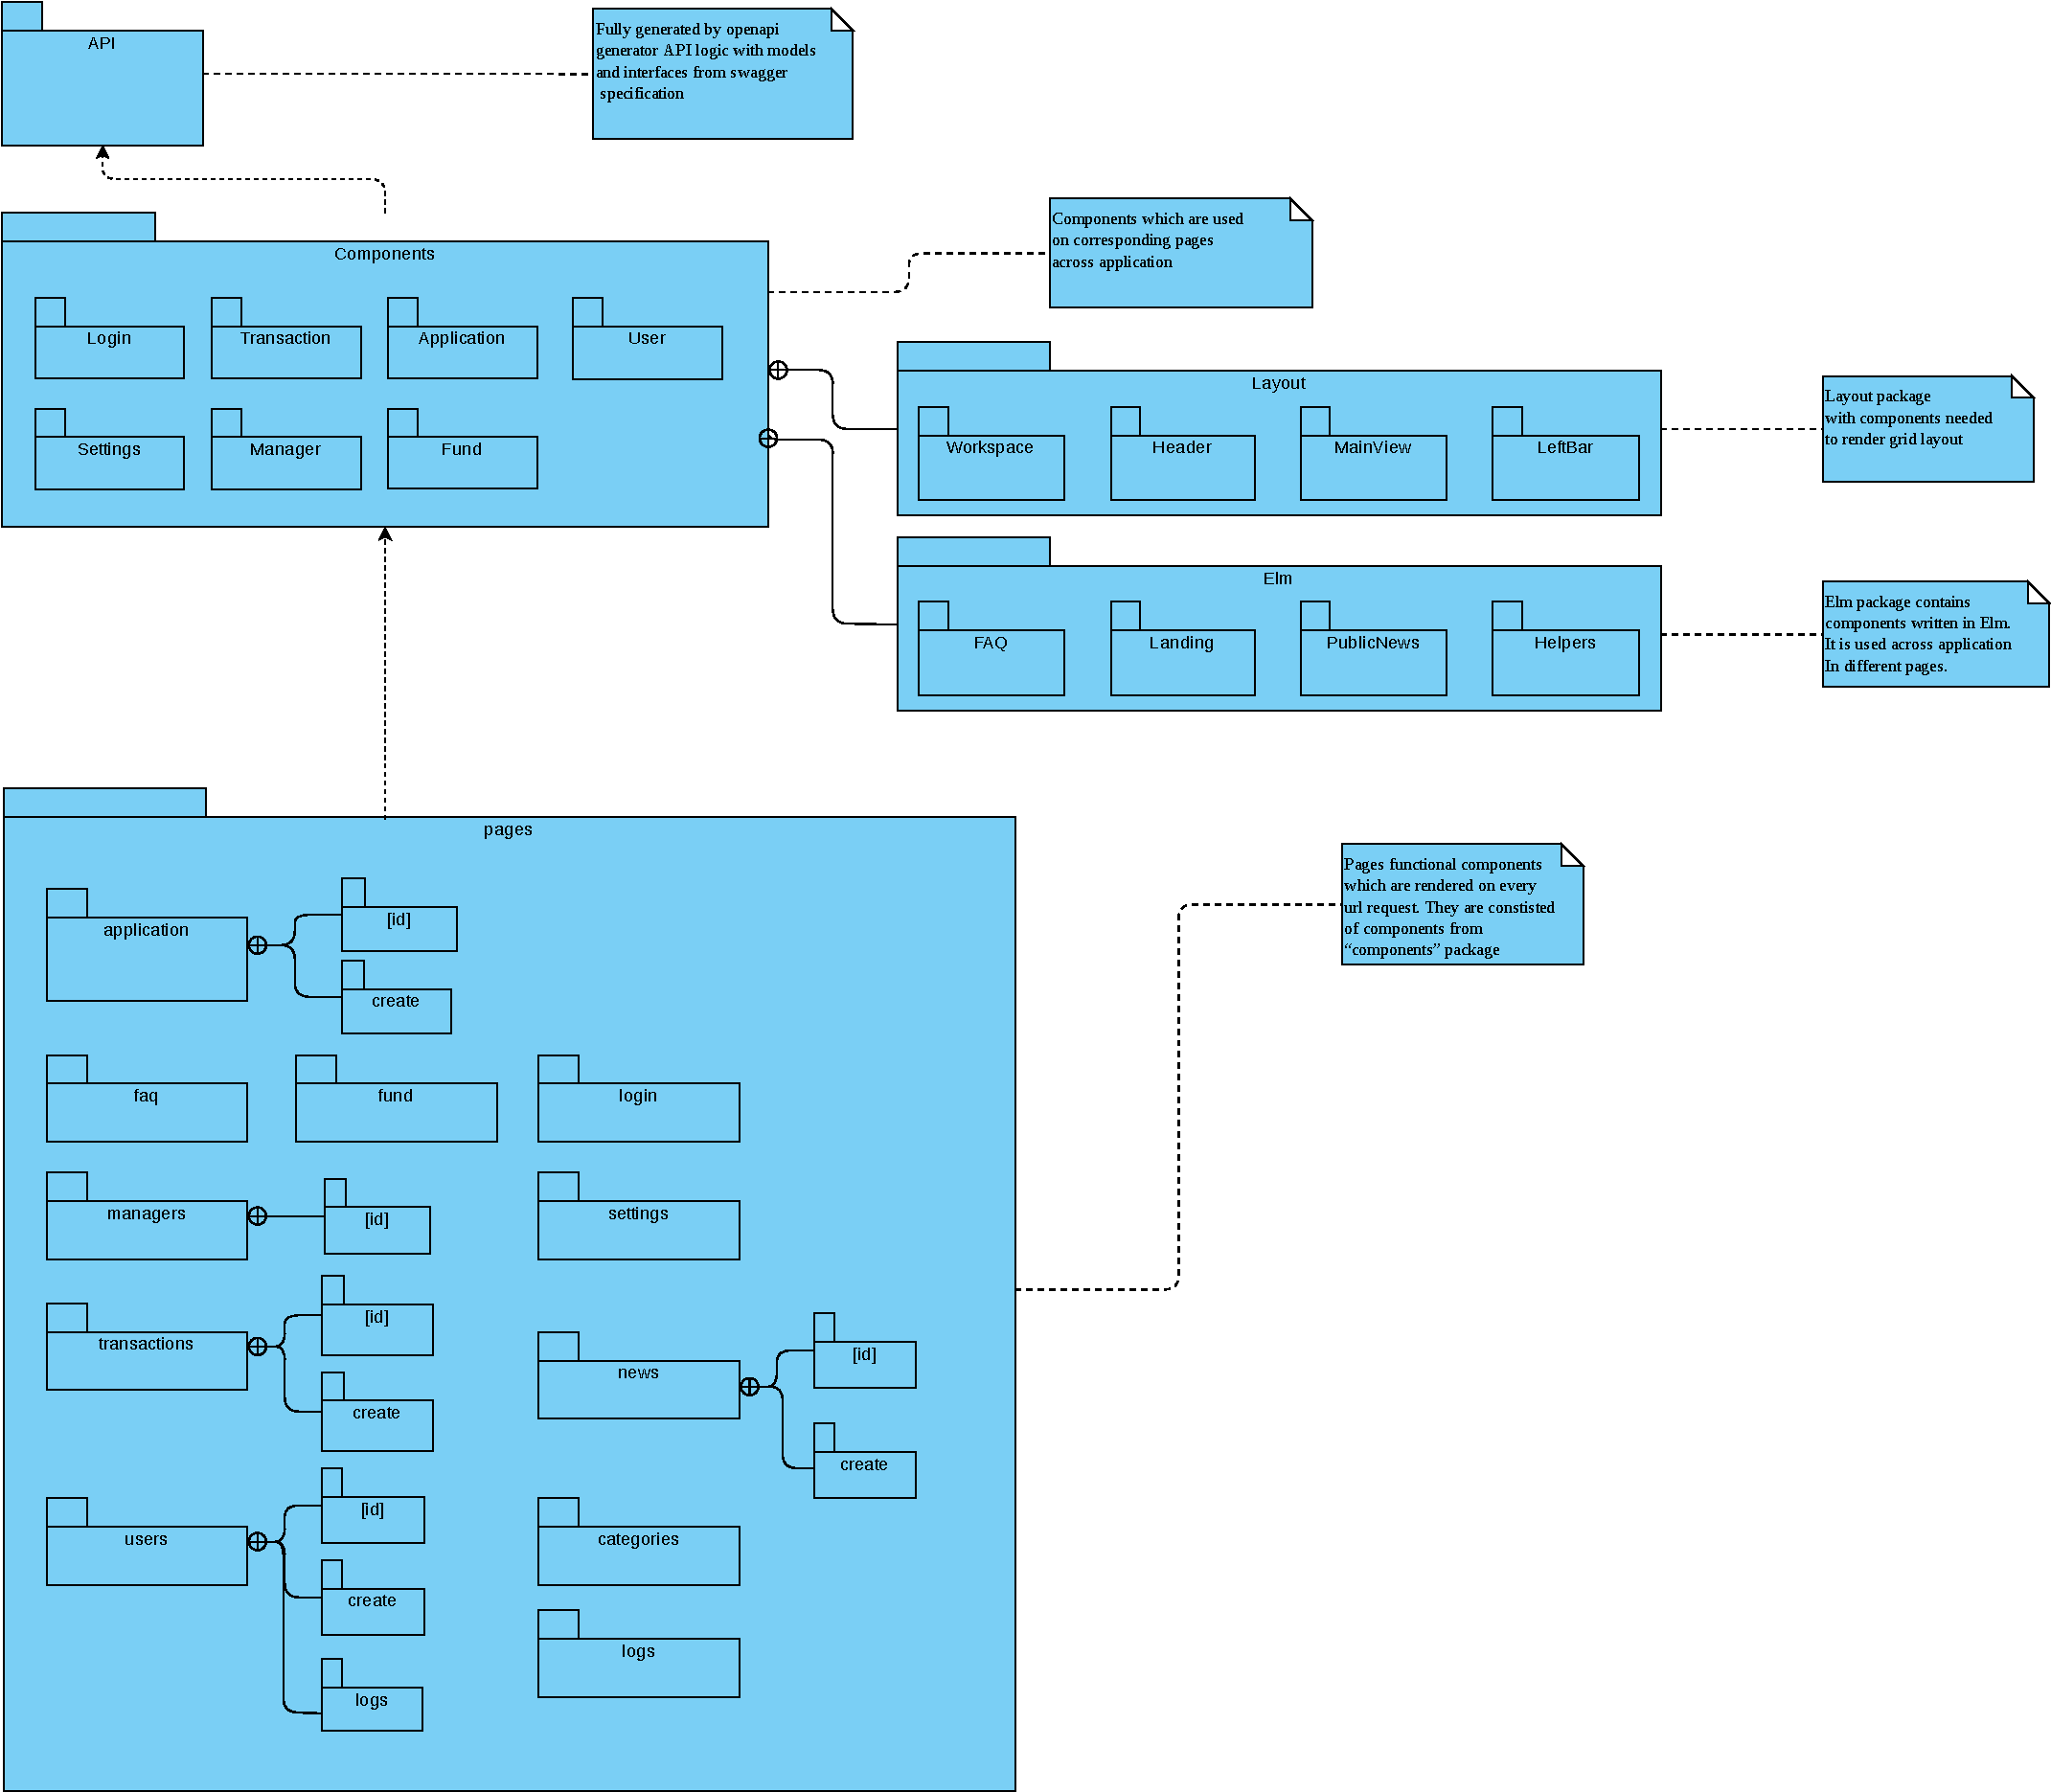
\includegraphics[width = 0.9\linewidth]{img/components.pdf}
		\caption{Диаграмма компонентов}
		\label{pic: component}
\end{figure}



\subsection{Диаграмма развертывания}

При проектировании диаграммы развертывания Web-приложения были использованы стандарты UML~\cite{uml}. 

Перед разработкой программы были составлены требования к информационной и программной совместимости, а также функциональные требования (см. Приложение \ref{additiontz}). Руководствуясь этими требованиями была составлена диаграмма развертывания, изображенная на рисунке \ref{pic: deployment}. Компоненты, отмеченные белым цветом на диаграмме, \texttt{Charity CRM Backend} и \texttt{Blockchain Server} были разработаны К. И. Манежиным и И. И. Костюченко соответственно. Так как оба сервиса нужны для корректной работы клиент-серверного приложения, то они отображены на диаграмме развертывания.

Для развертывания клиент-серверного приложения использовалась Host VM - виртуальная машина, предоставленная научным руководителем. Как можно увидеть на диаграмме \ref{pic: deployment}, на персональном компьютере взаимодействие с программой происходит через браузер с поддержкой HTML5 посредством канала связи HTTP непосредственно с Host VM. Как можно увидеть, на самой хостовой машине находится компонент \texttt{Web frontend Server}, который содержит внутри NGINX - компонент проксирования запросов и ReactAPP - само разработанное приложение. Через NGINX проксируются запросы на вышеупомянутый сервер \texttt{Charity CRM Backend} по API~\cite{api}.



\begin{figure}[H]
		\centering
		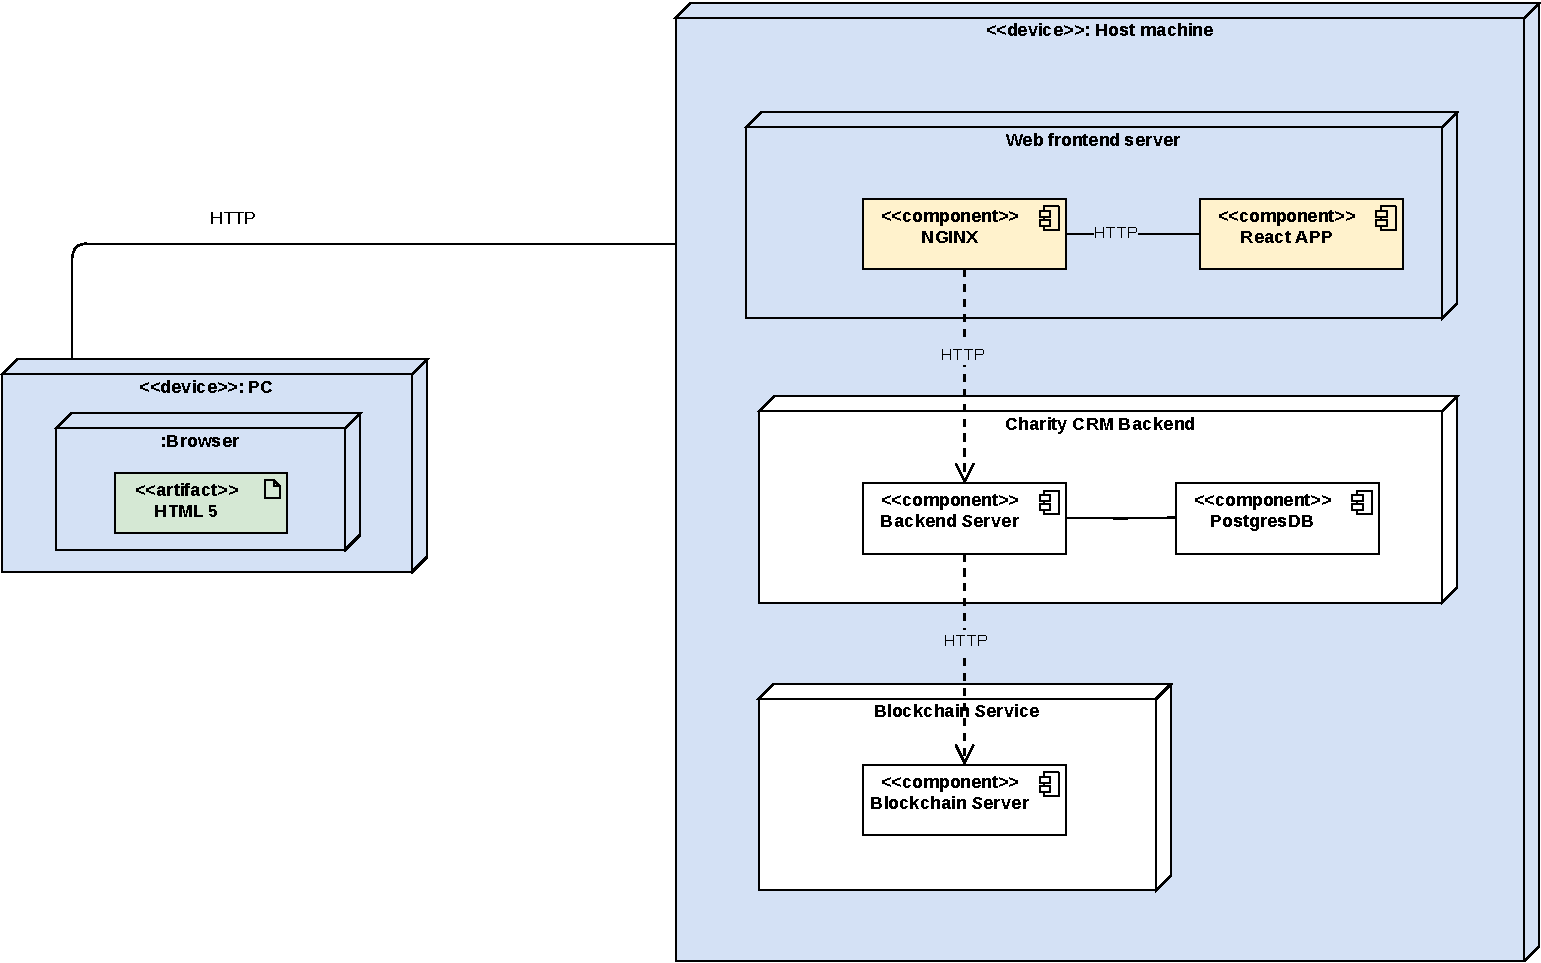
\includegraphics[width = 0.9\linewidth]{img/Deployment-Web.pdf}
		\caption{Диаграмма развертывания}
		\label{pic: deployment}
\end{figure}

Для автоматизации развертывания стабильных версий приложения был настроен CI/CD pipeline в Gitlab репозитории, состоящий из следующих шагов: eslint, prettier (линтеры кода), test (unit-тесты), build (сборка проекта) и deploy. Первые 4 шага должны быть пройдены успешно, прежде чем начался шаг deploy: сборка и развертывание проекта с помощью Docker контейнеров. Таким образом развертывание на хост-машине происходило автоматически при мердже в ветку develop, тест-стенд доступен по адресу \url{https://charity.infostrategic.com}. Также для удобства тестирования стабильной версии заказчиком был развернут master стенд на по адресу \url{https://charity2.infostrategic.com}.

\subsection{Диаграммы последовательности}

\subsubsection{Обработка заявки} \label{sec: sequence_status}

При составлении диаграммы последовательности бизнес процесса обработки заявок (представлен в разделе \ref{sec: bpmn_status} были выявлены следующие акторы: \texttt{Donee} - нуждающийся, пользователь мобильного приложения и \texttt{Comittee} - член комиссии, сотрудник фонда и пользователь Web-интерфейса. Нуждающийся через интерфейс \texttt{Android UI} взаимодействует с \texttt{ApplicationAPI},  а член комиссии через интерфейс \texttt{WebUI} также взаимодействует с \texttt{ApplicationAPI}. В свою очередь \texttt{ApplicationAPI} (API с эндпойнтами обработки заявок) взаимодействует с \texttt{ApplicationDBO} (класс, представляющий взаимодействие с базой данных) и \texttt{Blockchain module} (модуль блокчейна). 

Последовательность обработки заявки иницирует нуждающийся (Donee), который через интерфейс \texttt{AndroidUI} заполняет форму новой заявки и отправляет ее на обработку сотрудникам фонда посредством отправки запроса к \texttt{ApplicationAPI}. Член комисии фонда через Web-интерфейс \texttt{WebUI} после занесения заявки в базу данных видит ее в своем интерфейсе и берет заявку в обработку (переводит с помощью UI заявку в статус <<В обработке>>). Это действие регистрируется в базе данных через \texttt{ApplicationAPI}. После валидации данных заявки, если члена комисии все устраивает, то он отправляет заявку на подтверждение комисии (т.е переводит ее в новый статус <<Ждет подтверждения комисии>>). Изменения также регистрируются в базе данных посредством совершения запроса от \texttt{WebUI} к \texttt{ApplicationAPI}. После процесса голосования (данная диаграмма последовательности рассматривается в разделе \ref{sec: vote_seq}) менеджер переводит заявку в следующий статус <<На подтверждении пользователя>>. Нудающийся в свою очередь своим действием через \texttt{AndroidUI} активирует заявку, что фиксируется в системе блокчейн. 

\begin{figure}[H]
		\centering
		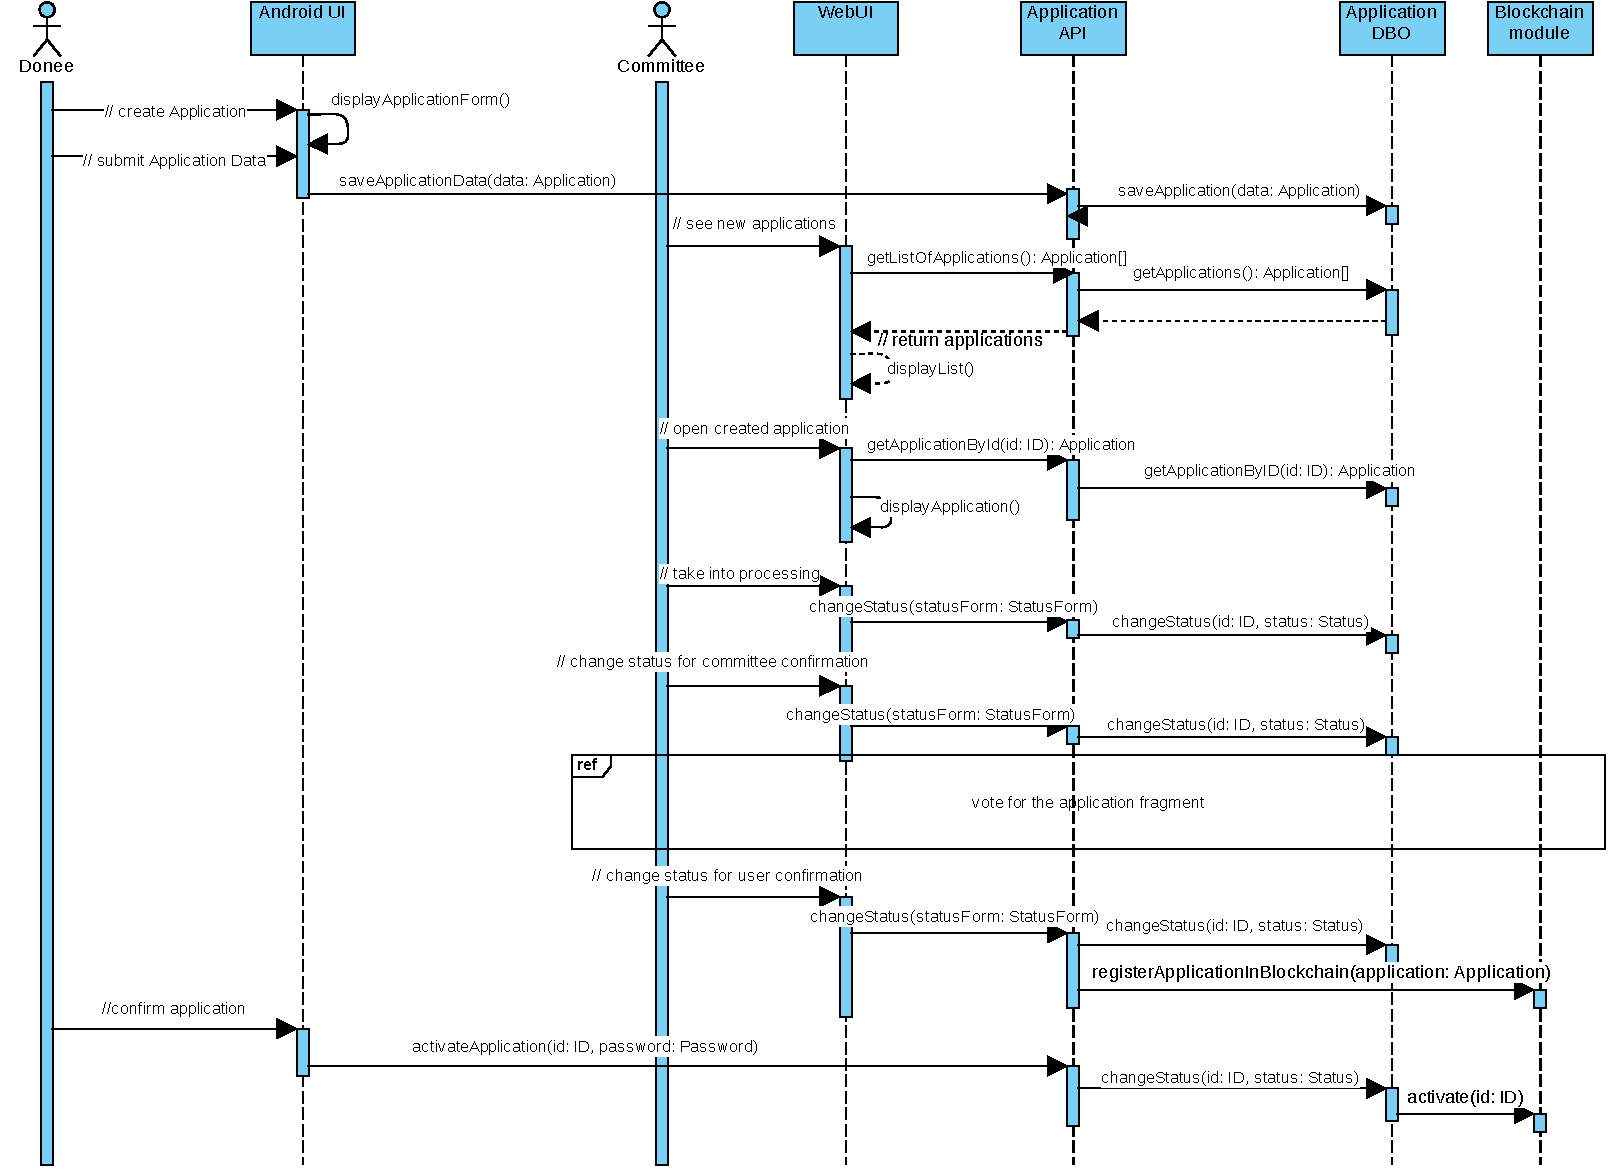
\includegraphics[width = \linewidth]{img/status_seq.pdf}
		\caption{Диаграмма последовательности обработки заявки}
		\label{pic: sequence_status}
\end{figure}


\subsubsection{Голосование по заявке} \label{sec: vote_seq}

При составлении диаграммы последовательности бизнес процесса обработки заявок (представлен в разделе \ref{sec: vote} были выявлены следующие акторы: Committee - член комиссии фонда; Член комиссии через Web-интерфейс отправляет запросы в \texttt{API}, которое регистрирует изменения в базе данных (представлена паттерном DAO - Data Base Object, \texttt{VoteDAO}, \texttt{ApplicationDAO}).

Последовательность голосования по заявке иницирует член комиссии, открывая карточку заявки в статусе <<Ждет подтверждения комисии>>. Именно по заявке в таком статусе может быть совершено голосование и принято решение по активации заявки.  После открытия карточки заявки происходит проверка: может ли член комиссии голосовать по данной заявке. Если назначенные категории члена комиссии совпадают с категорией заявки, то он может принимать решение по активации данной заявки. В противном случае член комиссии может только увидеть статистику голосов других сотрудников. Если же все-таки у члена комиссии есть право отдать голос за заявку, то он голосует с помощью UI и его голос регистрируется в системе. После того, как все ревьюеры проголосуют за или против заявки, ее уже можно будет перевести в статус <<На подтверждении пользователя>> или <<Отказано>>.  

\begin{figure}[H]
		\centering
		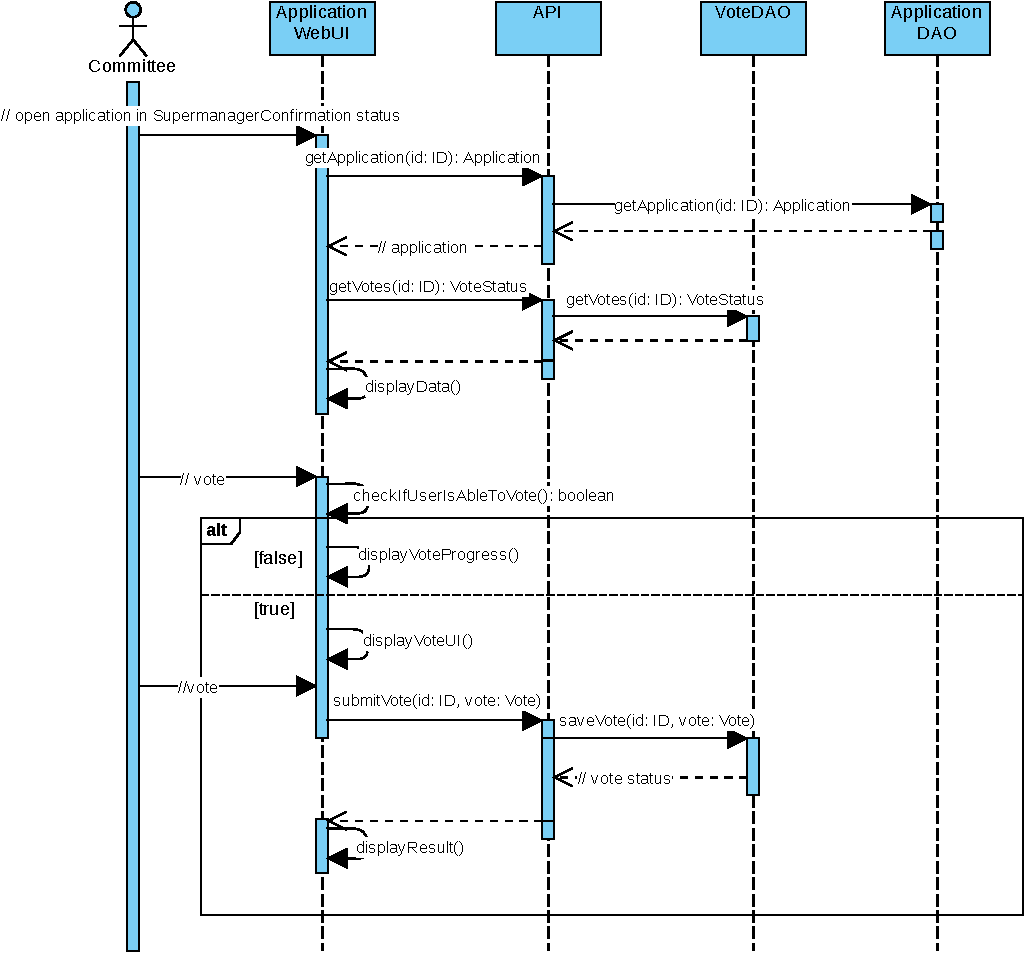
\includegraphics[width = 0.95\linewidth]{img/vote_seq.pdf}
		\caption{Диаграмма последовательности голосования по заявке}
		\label{pic: sequence_vote}
\end{figure}


\subsection{Реализация ролевой модели}

Как было упомянуто ранее в разделе \ref{theory-rbac}, разарабатываемое приложение включает в себя интерфейс и логику взаимодействия для пользователей с разными уровнями доступа - сотрудниками фонда.

Пользователи клиентского Web-приложения могут иметь следующие роли в системе: 

\begin{itemize}
    \item Admin - роль для администратора фонда;
    \item Supermanager - роль для члена комиссии фонда;
    \item Manager - роль для менеджера фонда;
    \item Operator - роль для оператора чата поддержки фонда;
    \item Content-manager - роль для менеджера контента фонда;
    \item Visitor - неавторизованный посетитель сайта;
\end{itemize}

Более подробное описание должностей сотрудников фонда представлено в приложении \ref{stuff}.

При проектировании реализации ролевой модели в Web-приложении использовался подход \texttt{Role-Based Access Control}~\cite{rbac}, описанный в разделе \ref{theory-rbac}. 

Первым шагом в реализации подхода была составлена таблица (см. Приложение \ref{rbac}) разделения возможностей, соответствующая функциональным требованиям (см. Приложение \ref{additiontz}) и прецедентам, описанным в разделе \ref{usecase}. По данной таблице был составлен следующий словарь, отображающий маппинг вышеперечисленных ролей на доступный функционал (см. Приложение \ref{rbac-ts}). Для того, чтобы определить, может ли пользовать с данной ролью получить доступ к странице или совершить какое-то действие, требующее особых прав, была разработан обработчик \ref{lst:check} для проверки уровня доступа к функциям.

\begin{lstlisting}[frame=single, basicstyle=\footnotesize\ttfamily, label={lst:check}, caption={Check функция для проверки уровня доступа},captionpos=b]
export function check(role: Role, action: string): boolean {
  const permissions = rules[role];
  if (!permissions) {
    // role is not present in the rules
    return false;
  }

  const staticPermissions = permissions.static;

  if (staticPermissions && staticPermissions.includes(action)) {
    // static rule not provided for action
    return true;
  }

  return false;
}

\end{lstlisting}

Далее был разработан React компонент (см. листинг \ref{lst:switch}), который на осбнове обработчика \texttt{check} (см. листинг \ref{lst:check}) принимает решение какой из компонентов рендерить на UI.

\begin{lstlisting}[frame=single, basicstyle=\footnotesize\ttfamily, label={lst:switch}, caption={RoleSwitch React компонент},captionpos=b]
import { FC } from "react";
import { check, Role } from "@providers/rbac-rules";

type RoleSwitchProps = {
  role: Role;
  perform: string;
  yes?: () => JSX.Element;
  no?: () => JSX.Element;
};

const RoleSwitch: FC<RoleSwitchProps> = ({
  role,
  perform,
  yes = () => null,
  no = () => null,
}) => (check(role, perform) ? yes() : no());

export default RoleSwitch;
\end{lstlisting}



\subsection{Используемые паттерны}

Приложение разрабатывалось с использованием технологии Single Page Application(далее - SPA)\cite{spa}. Ключевой особенностью является отсутствие перезагрузок страницы. То есть приложение напоминает нативное приложение под одну из операционных систем. Весь исполняемый код хранится у клиента, а не подгружается со стороннего сервера по необходимости (Server Side Rendering).

В процессе разработки WebUI для CRM Charity были использованы следующие паттерны проектирования:
\begin{itemize}
    \item Singleton — шаблон проектирования создания, который использовался для инициализации инстансов Axios\cite{axios} (библиотека для выполнения запросов). На диаграмме \ref{pic: singleton} изображен пример использования данного паттерна в проекте.
    
    \begin{figure}[H]
		\centering
		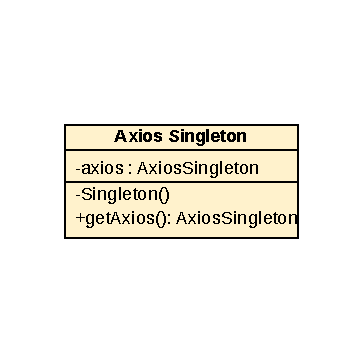
\includegraphics[width = 0.5\linewidth]{img/GoF_Singleton.pdf}
		\caption{Пример использования паттерна <<Singleton>>}
		\label{pic: singleton}
    \end{figure}

    \item Factory — шаблон проектирования создания, использовался при кодогенерации запросов к API с помощью спецификации openapi\cite{openapi} и документации swagger\cite{api}. На диаграмме \ref{pic: factory} изображен пример использования данного паттерна в проекте.
    
    \begin{figure}[H]
		\centering
		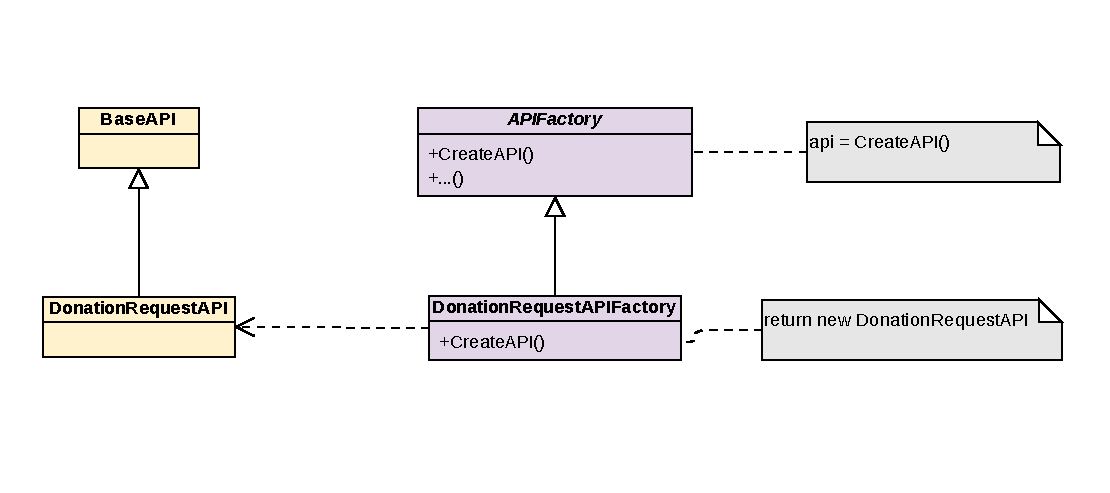
\includegraphics[width = 0.9\linewidth]{img/GoF_Factory.pdf}
		\caption{Пример использования паттерна <<Factory>>}
		\label{pic: factory}
    \end{figure}
    
    \item State — поведенческий шаблон проектирования, который позволяет объекту изменять свое поведение при изменении его внутреннего состояния. Данный шаблон использовался часто в разработке компонент web-приложения, так как React framework имеет встроенный механизм работы с State в компонентах (для классовых components уже имеется встроенные \texttt{this.state}, \texttt{this.setState}, для  \texttt{Factional Components} можно использовать механизм \texttt{React-hooks}\footnote{\url{https://reactjs.org/docs/hooks-overview.html}}, а именно \texttt{useState hook}\footnote{\url{https://reactjs.org/docs/hooks-state.html}}).
    
    \item MVU - структурный шаблон проектирования, который использовался при разработке Elm части Web-приложения. Разработка Web-страницы или компонента, написанного на Elm, делалилась на три части: model - состояние приложения, view - способ отрисовки в HTML, update - обновление состояния, основанное на полчении и отправке сообщений. На диаграмме \ref{pic: elm} изображен базовый пример использования паттерна в приложении: Html - отрисовка нового изображения согласно полученному update (Msg), а на экране комьютера можно видеть состояние модели в данный момент.
     
    \begin{figure}[h!]
		\centering
		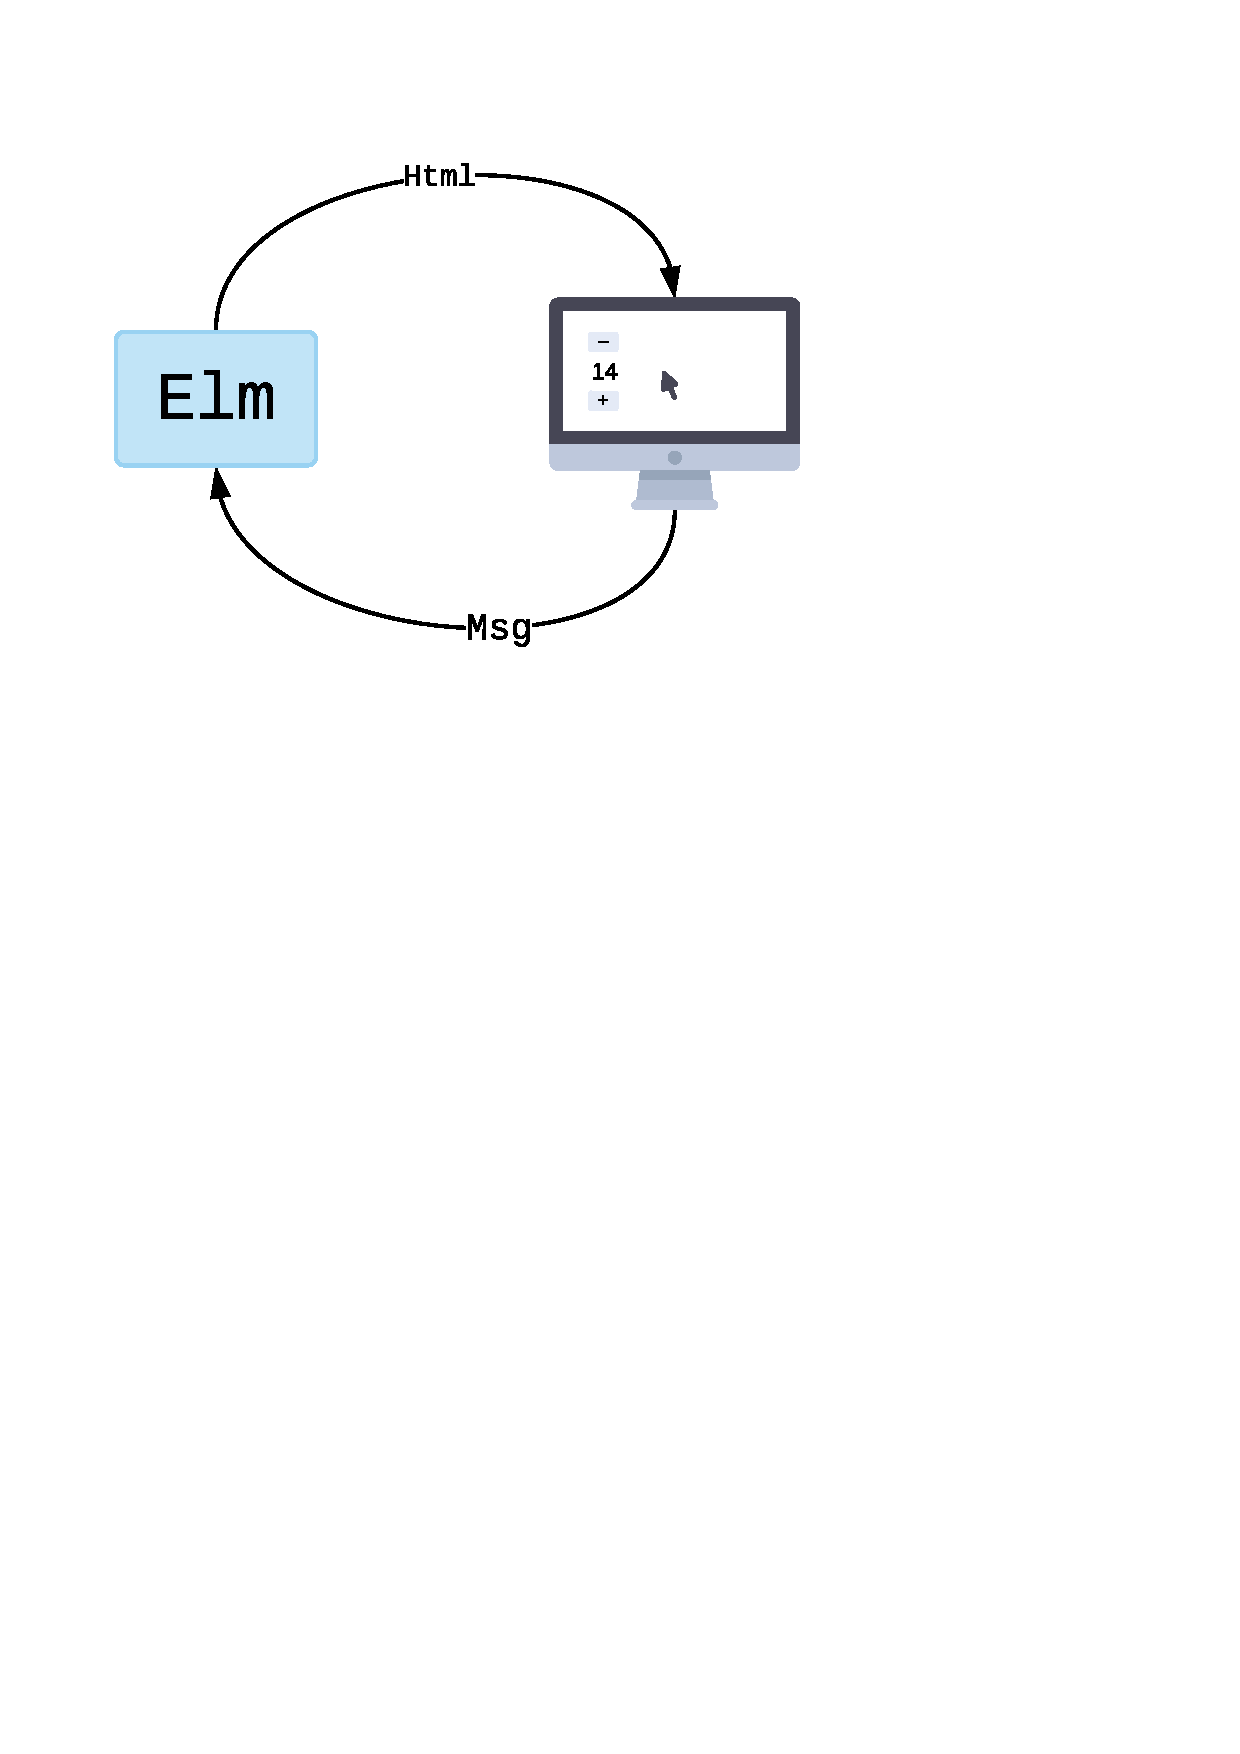
\includegraphics[width = 0.6\linewidth]{img/mvu.pdf}
		\caption{Базовый шаблон проектирования Elm приложений}
		\label{pic: elm}
    \end{figure} 
\end{itemize}


\anonsubsection{Выводы по главе}

При проектировании решения был проведен глубокий анализ технологий (представлен в разделе \ref{sec: tech}): были выбраны языки разработки Elm и Typescript (подробнее в разделе \ref{sec:lang}), а также фреймворк React для написания Web-приложения. Во время этапа проектирования были выбраны также библиотеки для разработки как для стека Elm, так и React+Typescript (подробнее в разделе \ref{sec: libr}). При проектировании приложения была разработана дизайн модель \ref{pic: designmodel} и диаграмма компонентов \ref{pic: component}, отображающие структуру разрабатываемого приложения. 

\anonsection{Заключение}

По итогам данной работы было написано Web-приложение для сотрудников фонда <<AIAIN>>, которое является частью CRM-системы для вышеупомянутого фонда. Весь заявленный функционал был реализован, автоматизация необходимых бизнес-процессов обеспечена. 

В рамках данной работы был проведен подробный анализ существующих аналогов, выявлены сильные и слабые стороны решений на рынке. После проведенного анализа и сбора требований заказчика были составлены функциональные требования, в которых был отражен весь необходимый функционал для Web-приложения. 

Перед разработкой был проведен этап анализа и проектирования, во время которых были построены диаграммы прецедентов и предметной области, а также выстроены ключевые бизнес-процессы по обработке заявок, голосованию и совершению сбора закята.

Одной из сильних сторон реализованого приложения является объединение и реализация ключевых бизнес-процессов в одном месте. Разработанный Web-интерфейс позволил объединить как администрирование пользователей, так и функциональность чатов поддержки, обработки заявок и управление контентов фонда -- и все в одном месте. Каждый сотрудник фонда теперь сможет пользоваться данной системой, что позволит сэкономить время и автоматизировать работу.

В будущем развитии проекта необходимо подключить банковскую систему для совершения платежей, переводов денежных средств. Еще одним вектором развития приложения является интернализация веб-интерфейса на арабский язык. Также в будущем планируется добавить следующий функционал: создание заявок от пользователей через Web-интерфейс, расширение аналитики.

Данная работа была представлена на конференции CoCoS 2021, 16.04.2021. Работа заняла 2 место в прикладном треке~\cite{cocos}.

\newpage
	%\section{Источники, использованные при разработке}
	%\renewcommand{\refname}{Список источников}
	% \addcontentsline{toc}{subsection}{\refname}
	\patchcmd{\thebibliography}{\section*{\refname}}{}{}{}
	\anonsection{Список источников}
	\begin{thebibliography}{27}
	    \bibitem{statistics} Digital population worldwide URL:\url{ttps://www.statista.com/statistics/617136/digital-population-worldwide/} [Электронный ресурс] (Дата обращения: 16.11.2020, режим доступа: свободный)
	    \bibitem{ieee} Saleh H., Sergey Avdoshin, Azamat Dzhonov. Platform for Tracking Donations of Charitable Foundations based on Blockchain Technology, in: Actual Problems of Systems and Software Engineering APSSE 2019 (Invited Papers). Los Alamitos, Washington, Tokyo : IEEE Computer Society, 2019. P. 182-187 [Электронный ресурс] URL:\url{https://ieeexplore.ieee.org/document/8943788} (Дата обращения: 16.11.2020, режим доступа: свободный)

	    
	    \bibitem{runok} How to attract donors? URL:\url{https://www.entrepreneur.com/article/233106} (Дата обращения: 16.11.2020, режим доступа: свободный)
	    \bibitem{competitors} How to identify your competitors? - ONCE Interactive [Электронный ресурс] URL:\url{https://onceinteractive.com/blog/how-to-identify-your-competitors/} (Дата обращения: 26.04.2021, режим доступа: свободный)
	    \bibitem{researchcrm} 
		Fundraising magazine crm survey, 2020 [Электронный ресурс] URL: 
		\url{https://www.beaconcrm.org/offer/fundraising-magazine-crm-survey-2020} (Дата обращения: 16.04.2021, режим доступа: свободный)
		\bibitem{uml} ГОСТ Р ИСО 15745-1-2014 URL:\url{https://docs.cntd.ru/document/1200119214} (Дата обращения: 26.04.2021, режим доступа: свободный)
		\bibitem{gost}Единая система программной документации – М.: ИПК, Издательство стандартов, 2000, 125 стр.
		\bibitem{lms} 
		LMS [Электронный ресурс] URL: 
		\url{https://lms.hse.ru} (Дата обращения: 16.11.2020, режим доступа: свободный)
		\bibitem{json} JSON [Электронный ресурс] URL: \url{https://www.json.org} (Дата обращения: 16.11.2020, режим доступа: свободный)
		
		\bibitem{webapp} Top 7 Languages for Web App Development [Электронный ресурс] URL: \url{https://fortyseven47.com/news/top-7-languages-for-web-app-development/} (Дата обращения: 16.04.2021, режим доступа: свободный)
		\bibitem{md} Markdown Guide URL: \url{https://www.markdownguide.org} (Дата обращения: 16.04.2021).
		\bibitem{api} Swagger Charity API, v0.2 [Электронный ресурс] (Дата обращения: 31.05.2021, режим доступа: свободный) URL:\url{https://app.swaggerhub.com/apis/charity-crm/Charity/0.2}
		\bibitem{mostpoplang} The best Web-application development languages in 2021 [Электронный ресурс] (Дата обращения: 31.05.2021, режим доступа: свободный) URL:\url{https://medium.com/@inverita/the-best-web-application-development-languages-in-2021-6b6eb5944925}
		
		\bibitem{rbac} Role-Based Access Control, Auth0  [Электронный ресурс] (Дата обращения: 31.05.2021, режим доступа: свободный) URL:\url{https://auth0.com/docs/authorization/rbac/#Handling-Authorization-in-React-Apps--the-Naive-Way}
		
		\bibitem{performance} React-Angular-Elm-Ember performance comparison [Электронный ресурс] (Дата обращения: 31.05.2021, режим доступа: свободный) URL:\url{https://github.com/evancz/react-angular-ember-elm-performance-comparison/blob/master/readme.md}
		\bibitem{assets} Elm lang - small assets without the headache [Электронный ресурс] (Дата обращения: 31.05.2021, режим доступа: свободный) URL:\url{https://elm-lang.org/news/small-assets-without-the-headache}
		\bibitem{elm-ports} Elm lang - Ports [Электронный ресурс] (Дата обращения: 31.05.2021, режим доступа: свободный) URL:\url{https://guide.elm-lang.org/interop/ports.html}
		\bibitem{ts-frameworks} RealWorldApp - Typescript [Электронный ресурс] (Дата обращения 31.05.2021, режим доступа: свободный) URL: \url{https://codebase.show/projects/realworld?category=frontend&language=typescript}
		
		\bibitem{realworld} A RealWorld Comparison 2020 [Электронный ресурс] (Дата обращения 31.05.2021, режим доступа: свободный) URL: \url{https://medium.com/dailyjs/a-realworld-comparison-of-front-end-frameworks-2020-4e50655fe4c1}
		
		\bibitem{bpmn} Business Process Model and Notation - Wikipedia [Электронный ресурс] (Дата обращения 31.05.2021, режим доступа: свободный) URL:\url{https://en.wikipedia.org/wiki/Business_Process_Model_and_Notation}
		
		\bibitem{cool} State of JS 2020 [Электронный ресурс] (Дата обращения 31.05.2021, режим доступа: свободный) URL:\url{https://2020.stateofjs.com/en-US/technologies/front-end-frameworks/}
		
		\bibitem{axios} Axios - Promise based library [Электронный ресурс] (Дата обращения 31.05.2021, режим доступа: свободный) URL:\url{https://github.com/axios/axios}
		
		\bibitem{curi} Curi Router - Documentation [Электронный ресурс] (Дата обращения 31.05.2021, режим доступа: свободный) URL:\url{https://curi.js.org}
		
		\bibitem{openapi} OpenAPI - Codegen [Электронный ресурс] (Дата обращения 31.05.2021, режим доступа: свободный) URL:\url{https://github.com/OpenAPITools/openapi-generator}
		
		\bibitem{rest} REST - Wikipedia [Электронный ресурс] (Дата обращения 31.05.2021, режим доступа: свободный) URL:\url{https://en.wikipedia.org/wiki/Representational_state_transfer}
		
		\bibitem{swaggerhub} SwaggerHub - Swagger API [Электронный ресурс] (Дата обращения 31.05.2021, режим доступа: свободный) URL:\url{https://app.swaggerhub.com/search}
		
		\bibitem{spa} SPA (Single-page application), MDN Web Docs [Электронный ресурс] (Дата обращения 31.05.2021, режим доступа: свободный) URL:\url{https://developer.mozilla.org/en-US/docs/Glossary/SPA}
		
		\bibitem{cocos} CoCoS 2021 - Дипломанты конференции [Электронный ресурс] (Дата обращения 31.05.2021, режим доступа: свободный) URL:\url{https://cs.hse.ru/studconf/2021/winners}
	\end{thebibliography}

\newpage

\addition{Техническое задание}{additiontz}
Представлено отдельным документом <<Техническое задание. CRM-система для благотворительного фонда <<AIAIN>>. Web-приложение для сотрудников фонда>>. 

\addition{Роли сотрудников фонда}{stuff}
\begin{description}
		\item[\textbf{Администратор}] -- это сотрудник фонда, который имеет доступ к функционалу по управлению пользователями системы.
		\item[\textbf{Член комиссии}] -- у каждого фонда есть комиссия, которая принимает итоговое решение об активации заявок от нуждающихся. В обязанности членов комиссии также входит обработка заявок, просмотр пожертвований поступающих от доноров, создание категорий для заявок и так далее.
		\item[\textbf{Контент-менеджер}] -- отвечает за управление контентом фонда, а именно: часто задаваемыми вопросами, основной информацией фонда и новостями фонда;
		\item[\textbf{Менеджер}] -- большая часть сотрудников фонда состоит из менеджеров фонда. В их обязанности входит только обработка заявок, коммуникация с пользователями и сбор необходимых документов если требуется;
		\item[\textbf{Оператор}] -- оператор фонда отвечает на вопросы пользователей мобильного приложения;
\end{description}
	
\addition{Role-based access control}{rbac}	
\begin{center}
\begin{longtable}{|p{0.2\linewidth}|p{0.2\linewidth}|p{0.05\linewidth}|p{0.05\linewidth}|p{0.05\linewidth}|p{0.05\linewidth}|p{0.05\linewidth}|p{0.05\linewidth}|}
\caption{Таблица с распределением возможностей пользователей по ролям} 
\label{table: rbac} \\

\hline
\multicolumn{1}{|c|}{\textbf{\tiny{Действие}}} &
\multicolumn{1}{c|}{\textbf{\tiny{Описание}}} &
\multicolumn{1}{c|}{\textbf{\tiny{Admin}}} & \multicolumn{1}{c|}{\textbf{\tiny{S.manager}}} &
\multicolumn{1}{c|}{\textbf{\tiny{Manager}}} & \multicolumn{1}{c|}{\textbf{\tiny{Operator}}} & \multicolumn{1}{c|}{\textbf{\tiny{C.manager}}} & \multicolumn{1}{c|}{\textbf{\tiny{Visitor}}} \\ \hline
\endfirsthead

\multicolumn{8}{r}%
{{ \tablename\ \thetable{} -- продолжение}} \\ 
\hline 
\multicolumn{1}{|c|}{\textbf{\tiny{Действие}}} &
\multicolumn{1}{c|}{\textbf{\tiny{Описание}}} &
\multicolumn{1}{c|}{\textbf{\tiny{Admin}}} & \multicolumn{1}{c|}{\textbf{\tiny{S.manager}}} &
\multicolumn{1}{c|}{\textbf{\tiny{Manager}}} & \multicolumn{1}{c|}{\textbf{\tiny{Operator}}} & \multicolumn{1}{c|}{\textbf{\tiny{C.manager}}} & \multicolumn{1}{c|}{\textbf{\tiny{Visitor}}} \\ 
\hline
\endhead

\multicolumn{8}{r}{{Продолжение на следующей странице}} \\ 
\endfoot

\hline 
\endlastfoot

\texttt{auth:login} & Авторизация & {\color{red}{НЕТ}} & {\color{red}{НЕТ}} & {\color{red}{НЕТ}} & {\color{red}{НЕТ}} & {\color{red}{НЕТ}} & {\color{green}{ДА}} \\ \hline

\texttt{faq:pretty} & Просмотр FAQ & {\color{red}{НЕТ}} & {\color{green}{ДА}} & {\color{red}{НЕТ}} & {\color{red}{НЕТ}} & {\color{green}{ДА}} & {\color{green}{ДА}} \\ \hline

\texttt{faq:edit} & Изменение FAQ & {\color{red}{НЕТ}} & {\color{red}{НЕТ}} & {\color{red}{НЕТ}} & {\color{red}{НЕТ}} & {\color{green}{ДА}} & {\color{red}{НЕТ}} \\ \hline

\texttt{fund:edit} & Изменение информации о фонде & {\color{red}{НЕТ}} & {\color{red}{НЕТ}} & {\color{red}{НЕТ}} & {\color{red}{НЕТ}} & {\color{green}{ДА}} & {\color{red}{НЕТ}} \\ \hline


\texttt{fund:description} & Просмотр информации о фонде & {\color{red}{НЕТ}} & {\color{green}{ДА}} & {\color{red}{НЕТ}} & {\color{red}{НЕТ}} & {\color{green}{ДА}} & {\color{green}{ДА}} \\ \hline

\texttt{fund:index} & Просмотр аналитики о фонде & {\color{red}{НЕТ}} & {\color{green}{ДА}} & {\color{red}{НЕТ}} & {\color{red}{НЕТ}} &  {\color{red}{НЕТ}} &  {\color{red}{НЕТ}} \\ \hline

\texttt{news:index} & Просмотр новостей о фонде & {\color{red}{НЕТ}} & {\color{red}{НЕТ}} & {\color{red}{НЕТ}} & {\color{red}{НЕТ}} & {\color{green}{ДА}} &  {\color{red}{НЕТ}} \\ \hline

\texttt{news:edit} & Изменение новостей о фонде & {\color{red}{НЕТ}} & {\color{red}{НЕТ}} & {\color{red}{НЕТ}} & {\color{red}{НЕТ}} & {\color{green}{ДА}} &  {\color{red}{НЕТ}} \\ \hline

\texttt{news:create} & Создание новостей о фонде & {\color{red}{НЕТ}} & {\color{red}{НЕТ}} & {\color{red}{НЕТ}} & {\color{red}{НЕТ}} & {\color{green}{ДА}} &  {\color{red}{НЕТ}} \\ \hline

\texttt{applications: show} & Просмотр заявки & {\color{red}{НЕТ}} & {\color{green}{ДА}} & {\color{green}{ДА}} & {\color{red}{НЕТ}} &  {\color{green}{ДА}} &  {\color{red}{НЕТ}} \\ \hline

\texttt{applications: create} & Создание заявки & {\color{red}{НЕТ}} & {\color{green}{ДА}} & {\color{green}{ДА}} & {\color{red}{НЕТ}} &  {\color{red}{НЕТ}} &  {\color{red}{НЕТ}} \\ \hline


\texttt{applications: index} & Просмотр списка заявок & {\color{red}{НЕТ}} & {\color{green}{ДА}} & {\color{green}{ДА}} & {\color{red}{НЕТ}} &  {\color{red}{НЕТ}} &  {\color{red}{НЕТ}} \\ \hline

\texttt{applications: edit} & Редактирование заявки & {\color{red}{НЕТ}} & {\color{green}{ДА}} & {\color{green}{ДА}} & {\color{red}{НЕТ}} &  {\color{red}{НЕТ}} &  {\color{red}{НЕТ}} \\ \hline

\texttt{applications: can-vote} & Голосование за активацию заявки & {\color{red}{НЕТ}} & {\color{green}{ДА}} & {\color{red}{НЕТ}} & {\color{red}{НЕТ}} &  {\color{red}{НЕТ}} &  {\color{red}{НЕТ}} \\ \hline

\texttt{categories: index} & Проосмотр, редактирование категорий & {\color{red}{НЕТ}} & {\color{green}{ДА}} & {\color{red}{НЕТ}} & {\color{red}{НЕТ}} &  {\color{red}{НЕТ}} &  {\color{red}{НЕТ}} \\ \hline

\texttt{transactions: index} & Список транзакций & {\color{red}{НЕТ}} & {\color{green}{ДА}} & {\color{red}{НЕТ}} & {\color{red}{НЕТ}} &  {\color{red}{НЕТ}} &  {\color{red}{НЕТ}} \\ \hline

\texttt{transactions: show} & Просмотр информации о транзакции & {\color{red}{НЕТ}} & {\color{green}{ДА}} & {\color{red}{НЕТ}} & {\color{red}{НЕТ}} &  {\color{red}{НЕТ}} &  {\color{red}{НЕТ}} \\ \hline

\texttt{transactions: create} & Создание ручной транзакции & {\color{red}{НЕТ}} & {\color{green}{ДА}} & {\color{red}{НЕТ}} & {\color{red}{НЕТ}} &  {\color{red}{НЕТ}} &  {\color{red}{НЕТ}} \\ \hline

\texttt{settings:index} & Изменение личного профиля & {\color{green}{ДА}} & {\color{green}{ДА}} & {\color{green}{ДА}} & {\color{green}{ДА}} &  {\color{green}{ДА}} &  {\color{red}{НЕТ}} \\ \hline

\texttt{settings:index} & Изменение личного профиля & {\color{green}{ДА}} & {\color{green}{ДА}} & {\color{green}{ДА}} & {\color{green}{ДА}} &  {\color{green}{ДА}} &  {\color{red}{НЕТ}} \\ \hline

\texttt{notifications: index} & Просмотр уведомлений & {\color{green}{ДА}} & {\color{green}{ДА}} & {\color{green}{ДА}} & {\color{green}{ДА}} &  {\color{green}{ДА}} &  {\color{red}{НЕТ}} \\ \hline

\texttt{users:show} & Просмотр профиля пользователя & {\color{green}{ДА}} & {\color{green}{ДА}} & {\color{green}{ДА}} & {\color{green}{ДА}} & {\color{red}{НЕТ}} &  {\color{red}{НЕТ}} \\ \hline


\texttt{users:index} & Просмотр списка пользователей системы & {\color{green}{ДА}} &  {\color{red}{НЕТ}} &  {\color{red}{НЕТ}} &  {\color{red}{НЕТ}} & {\color{red}{НЕТ}} &  {\color{red}{НЕТ}} \\ \hline

\texttt{users:create} & Регистрация пользователей в системе & {\color{green}{ДА}} &  {\color{red}{НЕТ}} &  {\color{red}{НЕТ}} &  {\color{red}{НЕТ}} & {\color{red}{НЕТ}} &  {\color{red}{НЕТ}} \\ \hline

\texttt{users:edit} & Изменение информации о пользователе & {\color{green}{ДА}} &  {\color{red}{НЕТ}} &  {\color{red}{НЕТ}} &  {\color{red}{НЕТ}} & {\color{red}{НЕТ}} &  {\color{red}{НЕТ}} \\ \hline

\texttt{logs:index} & Просмотр логов в системе & {\color{green}{ДА}} &  {\color{red}{НЕТ}} &  {\color{red}{НЕТ}} &  {\color{red}{НЕТ}} & {\color{red}{НЕТ}} &  {\color{red}{НЕТ}} \\ \hline

\texttt{managers:index} & Просмотр списка менеджеров системы &  {\color{red}{НЕТ}} &  {\color{green}{ДА}} &  {\color{red}{НЕТ}} &  {\color{red}{НЕТ}} & {\color{red}{НЕТ}} &  {\color{red}{НЕТ}} \\ \hline

\texttt{managers:show} & Просмотр профиля менеджера &  {\color{red}{НЕТ}} &  {\color{green}{ДА}} &  {\color{red}{НЕТ}} &  {\color{red}{НЕТ}} & {\color{red}{НЕТ}} &  {\color{red}{НЕТ}} \\ \hline

\texttt{managers:show} & Просмотр профиля менеджера &  {\color{red}{НЕТ}} &  {\color{green}{ДА}} &  {\color{red}{НЕТ}} &  {\color{red}{НЕТ}} & {\color{red}{НЕТ}} &  {\color{red}{НЕТ}} \\ \hline

\texttt{chat:show} & Просмотр диалога с пользователем &  {\color{red}{НЕТ}} &   {\color{red}{НЕТ}} &  {\color{red}{НЕТ}} &  {\color{red}{НЕТ}} & {\color{green}{ДА}} &  {\color{red}{НЕТ}} \\ \hline

\texttt{chat:index} & Просмотр списка диалогов с пользователем &  {\color{red}{НЕТ}} &   {\color{red}{НЕТ}} &  {\color{red}{НЕТ}} &  {\color{red}{НЕТ}} & {\color{green}{ДА}} &  {\color{red}{НЕТ}} \\ \hline


\end{longtable}
\end{center}

\addition{Реализация RBAC, rbac-rules.ts}{rbac-ts}	
\begin{lstlisting}[frame=single, basicstyle=\footnotesize\ttfamily, label={lst:POST}, caption={Словарь маппинга ролей на функциональность},captionpos=b]

export enum Role {
  visitor = "visitor",
  manager = "manager",
  supermanager = "supermanager",
  contentManager = "contentManager",
  operator = "operator",
  admin = "admin",
}

const rules = {
  visitor: {
    static: [
      "auth:login",
      "faq:pretty",
      "fund:description-pretty",
      "news:public",
    ],
  },
  contentManager: {
    static: [
      "applications:show",
      "settings:index",
      "users:show",
      "fund:index",
      "fund:faq-index",
      "fund:description",
      "fund:description-edit",
      "faq:edit",
      "news:edit",
      "news:create",
      "news:index",
      "notifications:index",
    ],
  },
  operator: {
    static: ["chats:show", "chats:index", "settings:index"],
  },
  manager: {
    static: [
      "applications:index",
      "settings:index",
      "application:edit",
      "applications:show",
      "applications:create",
      "users:show",
      "user:view-applications",
      "notifications:index",
    ],
  },
  supermanager: {
    static: [
      "applications:index",
      "applications:show",
      "application:edit",
      "application:can-vote",
      "applications:create",
      "settings:index",
      "categories:index",
      "users:show",
      "user:view-applications",
      "fund:index",
      "fund:description",
      "transactions:show",
      "transactions:index",
      "transactions:create",
      "managers:index",
      "managers:show",
      "fund:faq-index",
      "notifications:index",
      "transactions:distribute",
    ],
  },
  admin: {
    static: [
      "users:index",
      "users:show",
      "user:edit",
      "users:create",
      "user:view-sessions",
      "user:show-admin",
      "settings:index",
      "logs:index",
      "notifications:index",
    ],
  },
};

\end{lstlisting}


\end{document}